\documentclass[11pt,a4paper]{report}

% =========================
% Packages
% =========================
\usepackage{amsmath}
\usepackage{amssymb}
\usepackage{mathtools}
\usepackage{amsthm}
\usepackage{physics}
\usepackage{graphicx}
\usepackage{xcolor}
\usepackage{hyperref}
\usepackage{cleveref}
\setlength{\marginparwidth}{2cm}
\usepackage{comment}
\usepackage{stmaryrd}
\theoremstyle{definition}
\newtheorem{definition}{Definition}[section]


%TO DO
\usepackage[colorinlistoftodos]{todonotes}

\newcommand{\decide}[1]{%
  \todo[color=yellow!40]{DECIDE: #1}}

\newcommand{\supervisor}[1]{%
  \todo[color=blue!25]{Achilleas: #1}}

\newcommand{\cleanup}[1]{%
  \todo[color=green!25]{CLEAN UP: #1}}


\usepackage{listings}
\usepackage{caption}
\usepackage{subcaption}
\usepackage{tikz}
\usetikzlibrary{shapes.geometric, arrows.meta, positioning, fit, backgrounds}

% =========================
% Code style
% =========================
\lstset{
  basicstyle=\ttfamily\footnotesize,
  breaklines=true,
  frame=single,
  numbers=left,
  numberstyle=\tiny,
  showstringspaces=false,
  keywordstyle=\bfseries,
  commentstyle=\itshape,
  captionpos=b
}

\usepackage{minted}
\setminted{
  fontsize=\footnotesize,
  baselinestretch=1.15,
  linenos=false,
  frame=single,
  framesep=6pt,
  rulecolor=\color{gray!40},
  bgcolor=gray!6,
  breaklines=true,
  breakanywhere=false,
}
% Raw toolkit output (the `text' lexer) consists of long unbroken tensor
% monomials with no spaces to break at, so it needs mid-token breaking.
\setminted[text]{
  fontsize=\footnotesize,
  breakanywhere=true,
}



% --- Encoding & fonts ---
\usepackage[T1]{fontenc}
\usepackage[utf8]{inputenc}   % if not already set by your class

% --- Code highlighting (needs --shell-escape at compile time) ---

% --- Callout / info boxes ---
\usepackage{tcolorbox}
\tcbuselibrary{skins, breakable}

% --- Better tables ---
\usepackage{booktabs}
\usepackage{array}
\usepackage{longtable}

% --- Compact lists ---
\usepackage{enumitem}

% =========================
% Minted style and callout boxes (used from Chapter 1 onwards)
% =========================
\usemintedstyle{friendly}

\tcbset{
  feynbox/.style={
    enhanced, breakable,
    fonttitle=\bfseries\small,
    coltitle=black,
    boxrule=0.5pt,
    arc=3pt,
    left=8pt, right=8pt, top=6pt, bottom=6pt,
    parbox=false,
  },
  notebox/.style={
    feynbox,
    colframe=black!35,
    colback=black!4,
  },
  infobox/.style={
    feynbox,
    colframe=blue!45,
    colback=blue!4,
  },
  warnbox/.style={
    feynbox,
    colframe=orange!65,
    colback=orange!5,
  },
}

% Inline Python identifiers
\newcommand{\py}[1]{\mintinline{python}{#1}}

% Fixed-width parameter-table column
\newcolumntype{P}[1]{>{\ttfamily\small}p{#1}}


\title{Automatic Derivation of Feynman Rules from Symbolic Model Declarations}
\author{Remo}
\date{\today}

\begin{document}

\maketitle

\begin{abstract}
\noindent
Extracting Feynman rules from a Lagrangian is a mechanical but unforgiving
task, and for a theory such as the Standard Model Effective Field Theory,
with several hundred independent Wilson coefficients, it can no longer be
carried out by hand. The established solution is \textsc{FeynRules}, a
\textsc{Mathematica} package that derives vertices from a declarative model
file. This thesis asks whether the same service can be provided inside the
Python ecosystem, and answers it by building \textsc{FeynPy}: a toolkit in
which a user declares indices, fields, gauge groups and parameters as
ordinary Python objects, writes a Lagrangian in a notation close to the one
used on paper, and obtains tree-level Feynman rules as symbolic expressions.

The toolkit is built on \textsc{Symbolica} for symbolic algebra and on
\textsc{Spenso} for typed tensor indices. A declared Lagrangian is validated,
its implicit indices are resolved, and its gauge structure --- covariant
derivatives, field strengths, gauge fixing and ghosts --- is expanded into
local monomials that all meet at a single intermediate representation. A
contraction engine then realises the canonical-quantisation derivation of a
vertex as a pruned sum over permutations of the external legs, and a
canonicalisation layer reduces the result to a comparable normal form.

Correctness is established by direct algebraic comparison against
\textsc{FeynRules} exports. The packaged Standard Model matches at
$163/163$ vertices, the unbroken background-field Standard Model at $67/67$,
and the Green-basis SMEFT at $184/184$ reference lines, of which $161$ match
directly and the remainder after explicitly documented charge-conjugation
conventions. Deliberate mutation tests confirm that the comparison stays
sensitive to genuine changes in physical content.
\end{abstract}

\tableofcontents

% =========================
% Chapters
% =========================
% ============================================================
%  01_introduction.tex --- Introduction
% ============================================================

% ==============================================================
\chapter{Introduction}
\label{ch:introduction}
% ==============================================================

% --------------------------------------------------------------
\section{From a Lagrangian to a prediction}
\label{sec:intro-motivation}
% --------------------------------------------------------------

In particle physics, we are always searching for new theories, and the key to describing a system is its Lagrangian. A theory only becomes meaningful when it is corroborated by many experiments,\supervisor{[DONE] experiments (many)} and the experimentalist who wants to test that theory needs theoretical predictions: inclusive cross sections, differential distributions and other quantities that can be measured in a particle accelerator.\supervisor{[DONE] needs theoretical predictions: inclusive cross sections, differential distributions etc.} The first step towards a bridge\supervisor{[DONE] the bridge -> the first step towards a bridge} between the theory and those measurable quantities is the set of Feynman rules, the elementary vertices from which each amplitude is assembled.

This conversion is purely mechanical and algebraic. \Cref{sec:feynrules-algorithm} describes the algorithm\supervisor{[DONE] recipe->algorithm} in detail, but we can briefly summarize it as follows: take a term of the Lagrangian, add a creation operator for each field, commute the operators, replace each derivative with a momentum\supervisor{[DONE] momentum!}, and eliminate external wave functions. Precisely because these operations are always the same, it is so prone to being implemented algorithmically. Clearly, there are many ramifications and complications: each field carries Lorentz indices, spinors, color, weak isospin, and flavor that must be contracted with the correct partner; each covariant derivative expands into a term for each gauge group under which the field transforms; each field strength of a non-Abelian group splits into three parts, so a product of $n$ of them splits into $3^n$; each exchange of two fermions costs a sign, the convention of which must be established once and never violated again.

For a Lagrangian with few terms and few fields, performing these operations manually can already be quite tedious. For the Standard Model, it is a well-known exercise but indeed error-prone as the terms are numerous. Then we have theories that are both more complex and far larger,\supervisor{[DONE] what do you mean long-lived?} such as the Standard Model Effective Field Theory (SMEFT). This is the model used as the main benchmark for this thesis, which contains 32 Lagrangian blocks and 298 independent Wilson coefficients, and generates 184 distinct reference vertices with three to six external legs. Nowadays, no one derives it manually,\supervisor{[DONE] Nowadays,..} verifies it manually, or, more precisely, modifies an operator and recalculates it manually.

With the creation of new theories that have become increasingly complex, it became necessary to automate this process. Thus, FeynRules was born, a model that uses Mathematica to calculate Feynman's rules given a theory and its Lagrangian. Years passed, and many physicists wanted to stop working with mathematics, and thus the idea for this thesis was born: to develop a toolkit capable of calculating Feynman's rules in Python.

% --------------------------------------------------------------
\section{The state of the art}
\label{sec:intro-state-of-the-art}
% --------------------------------------------------------------



The reference implementation of this idea is
\textsc{FeynRules}~\cite{Christensen:2008py,Alloul:2013bka}, a
\textsc{Mathematica} package that has been a standard entry point for building models
for collider phenomenology for over a decade. Its workflow is the one
this thesis deliberately imitates, so it is worth specifying explicitly. The \textsc{FeynRules} workflow is briefly summarized below.

First, a \textsc{FeynRules} model file is created, which has a declarative structure. The user fills
\texttt{M\$ClassesDescription} with the particle content, specifying for each field
its spin, self-conjugation, indices, and quantum numbers; they fill
\texttt{M\$Parameters} with the parameters and mixing matrices; and declare
the gauge groups in \texttt{M\$GaugeGroups}, each with its own coupling,
gauge boson, structure constants, and representations. The Lagrangian
is then written as a normal \textsc{Mathematica} expression, using a small
vocabulary of symbols: \texttt{DC[...]} for a covariant derivative,
\texttt{FS[...]} for the field-strength tensor, \texttt{del[...]} for an ordinary derivative, and \texttt{Ga[...]} for a Dirac matrix. A single call to
\texttt{FeynmanRules[...]} returns the vertices, and a further call exports
the model in the UFO format, which is used by event generators such as \textsc{MadGraph5\_aMC@NLO}.

There are two main reasons why many physicists may wish to move away from \textsc{FeynRules}. The first is that it is based entirely on \textsc{Mathematica}. This presents some inconveniences, the main one being that it does not integrate naturally with the Python-based machine-learning and analysis stack that the field now relies on for much of its other work. The second issue is computational cost. When the theory becomes complicated or the Lagrangian contains a large number of terms, the required computation time can become very high. As an example, this thesis aimed to implement the SMEFT model, which in \textsc{FeynRules} requires about half an hour of wall-clock time to export its reference vertices, as recorded in
\Cref{tab:validation-performance}.

The gap this thesis aims to fill, therefore, isn't that the problem is unsolved or that a suitable toolkit doesn't already exist—not at all.
The point is that, until recently, there was no equivalent solution available in the Python ecosystem, where much of the remaining work is taking place.

% --------------------------------------------------------------
\section{Why Python, and why now}
\label{sec:intro-why-now}
% --------------------------------------------------------------

For a long time, Python was not an adequate environment for creating such a toolkit that could perform algebraic operations and, more importantly, understand the meaning of symbolic expressions such as tensor networks with typed indices, expanded over thousands of terms.

This changed, however, with the birth of Symbolica, a computer algebra system with a core written in Rust and, more importantly, a Python interface. It provides efficient manipulation of large symbolic expressions through pattern-based rewriting and a fast multivariate polynomial engine, allowing expressions containing thousands of terms to be transformed and normalized efficiently. What Symbolica does not provide by itself is the type information needed to interpret tensor indices.

Building on Symbolica, a very promising and capable library, \textsc{Spenso}~\cite{spenso}, was developed by Lucien Huber. This library adds the missing type information: it makes an
index not simply a name, but part of a slot that also carries a representation, so that the
library itself knows that a fundamental color index can contract with its
dual and not with a Lorentz index. A complementary layer, \textsc{idenso}, provides the
additional physical identities: metric contraction, the $\mathrm{SU}(N)$ color algebra, and the Dirac algebra.

Together, these three libraries provide exactly the services that a \textsc{FeynRules}-like tool needs and that Python previously lacked.
\Cref{ch:cas} describes them in detail. This thesis is, in a nutshell, an attempt to see how far these libraries can go by further developing them.

% --------------------------------------------------------------
\section{Contributions}
\label{sec:intro-contributions}
% --------------------------------------------------------------

This thesis presents \textsc{FeynPy}, a Python toolkit that derives
tree-level Feynman rules from declarative model definitions. Its
contributions are the following.

\begin{enumerate}
    \item \textbf{A declarative model language in plain Python.} Indices,
    fields, parameters, gauge representations and gauge groups are ordinary
    Python objects, and a Lagrangian is written as an ordinary Python
    expression in a notation deliberately close to the
    \textsc{FeynRules} one
    (\Cref{ch:feynpy}).

    \item \textbf{A generic gauge compiler.} Covariant derivatives, field
    strengths, gauge-fixing terms and Faddeev--Popov ghosts are expanded
    from the model's own gauge metadata.

    \item \textbf{A contraction engine with a controlled fermion-sign
    convention.} Vertices are produced by a pruned sum over permutations of
    the external legs, the direct realisation of the canonical-quantisation
    recipe.

    \item \textbf{A canonicalisation layer that makes cross-tool comparison
    possible.} Dummy relabelling, tensor symmetries, a deterministic
    generator-ordering rewrite and a restricted use of the Jacobi identity
    reduce two independently derived expressions to a common normal form
    (\Cref{sec:internals-postprocessing,sec:validation-canonical}). 

    \item \textbf{An operator calculus on compiled Lagrangians.} Operators
    can be applied to an already compiled Lagrangian.\supervisor{[DONE] Stuff $\to$ Operations } Field
    transformations implement electroweak symmetry breaking and the
    background-field split, and graded operators implement infinitesimal
    gauge variations and BRST transformations
    (\Cref{sec:feynpy-transformations,sec:feynpy-brst}).

    \item \textbf{A model-agnostic comparison framework, and three validated
    benchmarks.} The packaged Standard Model reproduces its
    \textsc{FeynRules} export at $163/163$ vertices; the unbroken
    background-field Standard Model at $67/67$; and the Green-basis SMEFT at
    $184/184$ reference lines, of which $161$ match directly and the rest
    after documented charge-conjugation conventions (\Cref{ch:validation}).
\end{enumerate}

% --------------------------------------------------------------
\section{Scope and limitations}
\label{sec:intro-scope}
% --------------------------------------------------------------

Finally, I would like to clearly specify the scope of this work so that the results in \Cref{ch:validation} are interpreted correctly.

\textsc{FeynPy} derives Feynman rules exclusively at tree level. It does not support loop corrections, counterterms, restriction files, or export to formats such as UFO, \textsc{FeynArts}, or \textsc{CalcHEP}. Integration by parts is currently limited to scalar fields.

As a result, validation is limited to the interaction vertices and does not cover the full model metadata or numerical parameter definitions.

Within these limits, however, the result is significant: for three complete, independently written models, the vertices produced by \textsc{FeynPy} agree algebraically with those produced by \textsc{FeynRules}. The precise scope and coverage of this validation are detailed in \Cref{sec:validation-coverage}.


% --------------------------------------------------------------
\section{Outline}
\label{sec:intro-outline}
% --------------------------------------------------------------

\Cref{ch:theory} aims to provide the theoretical foundation for understanding the canonical quantization, which is the functional basis of the algorithm implemented by feynpy. The chapter will address topics such as the role of symmetry, the Lie algebra mechanism that assigns fields to their indices, the structure of gauge Lagrangians, including gauge fixing, ghosts and spontaneous symmetry breaking, the logic of effective field theory and the SMEFT basis used later, and finally the canonical quantization algorithm that transforms a Lagrangian term into a vertex.

\Cref{ch:feynpy} serves as a user's manual. It builds a model from indices and fields to a complete QCD Lagrangian with gauge fixing, extracts its vertices. Additionally it describes the additional operations available on a compiled Lagrangian: field transformations
in a physical basis, gauge variations, BRST transformations,
and the included Standard Model and SMEFT implementations.

\Cref{ch:cas} introduces \textsc{Symbolica}, \textsc{Spenso}, and \textsc{idenso} and explains the small interface object that connects them to the toolkit.

\Cref{ch:internals} explains how the code works internally. It begins by explaining how to move from declarative classes to Wick's contraction engine and canonization, and then output the expression in Symbolica.

\Cref{ch:validation} provides validation between the models implemented in FeynRules and their counterparts in FeynPY. It then reports the three benchmark comparisons, examines the charge conjugation and chirality conventions that required attention, and demonstrates, through mutation tests, that the comparison is nontrivial.

\Cref{ch:conclusion} summarizes what has been accomplished, what proved challenging, and the next steps for the work.
\chapter{Theoretical Background}
\label{ch:theory}
\section{The beauty of Symmetry}

Over the centuries, physics has developed increasingly with the aim of understanding and describing the universe and its nature. One might think that mathematical complexity has increased steadily in order to describe the universe, and in a sense this is true, but how far have we gone? Is there a limit to the complexity we can achieve? Is there a risk, however remote, that physicists might lose control of this mathematical machine, which is becoming ever more complex and detached from any conceivable reality and, ultimately, from the physical world?

\noindent To answer this question, I would like to address the topic in physics that has most captured the author's attention: \textit{the role of symmetry.}


\subsubsection{Simplicity Behind Complexity}
\begin{center}
    `The bigger the puzzle, the harder it is to solve.'
\end{center}

There is certainly some truth in this statement. To put it into context, let's consider an example. If I wanted to describe a room, I would have to refer to every object inside it, and then specify its position and orientation. In short, I could spend hours describing a room in minute detail. If I then wanted to describe the entire flat, then move on to the building, and then go on to describe a city, the task would become increasingly complex. At this point, the more attentive readers will already have guessed where I'm heading.

Describing the universe seems an impossible task, unless we find a way to simply represent something far greater than anything simple. This is where physicists' interest in symmetries stems from.

Let's return to a concrete example: a beehive. I could make the task of describing it very long and tedious, scrutinising every single detail that makes it up. Or I could note a pattern that extends throughout the entire beehive. All I need to do is describe a single hexagon and then observe that, by symmetry, the rest of the beehive follows the same structure.

But what exactly is symmetry? We can define it in various ways; let's look at two of them. From an intuitive point of view, symmetry is a pattern that exhibits a certain regularity in space and time. From a physical point of view, we can define it as a property that remains unchanged following a transformation.

Thus begins the `hunt for symmetries' by physicists. I would like to mention some of the most common ones in physics. If we think of a wheel, it possesses rotational symmetry about an axis, the one passing through its hub. Another fundamental symmetry is temporal symmetry: if we shift a system forwards or backwards in time, the laws of physics must remain the same.  Without this symmetry, physics would be unable to make predictions and therefore formulate universal laws.

Nature possesses many other symmetries. There is, for example, reflection symmetry: like in a mirror, it allows us to recognise when a configuration remains equivalent to its reflected image.

In the next section, we will delve into the mathematics that allows us to describe this fundamental concept, which underpins the evolution of physics and, with it, our understanding of the universe.

\begin{comment}{
"The bigger the puzzle, the harder to solve."
 Asserzione che sicuramente ha del vero. Per contestualizzarla, consideriamo un esempio. Se volessi descrivere una stanza dovrei far riferimento ad ogni oggetto al suo interno, per poi specificarne la posizione e l'orientamento. Insomma potrei passare ore a descrivere minuziosamente una stanza. Se poi volessi descrivere l intero appartamento, per poi passare alla palazzina, per poi passare alla descrizione di una città, il compito diventerebbe sempre più complesso. A questo punto, i lettori più attenti avranno già intuito dove voglio arrivare.

Descrivere l'universo sembra un impresa irrangiungibile, a meno che non troviamo un escamotage per rappresentare con semplicità qualcosa di assai più grande che di semplice non ha nulla. Da qui nasce l'interesse dei fisici per le simmetrie.

Torniamo ad un esempio concreto, ovvero un alveare. Potrei rendere il compito di descriverlo molto lungo e tedioso, guardando miniziosamente ad ogni dettaglio che lo compone. Oppure potrei notare un pattern che si estende per tutto l'alveare. Mi basta descrivere un singolo esagono e poi osservare che, per simmetria, il resto dell'alveare segue la stessa struttura.

ma cosa è esattamente una simmetria? possiamo definirla in vari modi, vediamone due. Dal punto di vista intuitivo, una simmetria è un pattern che presenta una certa riccorenza nello spazio e nel tempo. Dal punto di vista fisico, possiamo definirla come una proprietà che rimane invariata in seguito a una trasformazione.

Inizia cosi la "caccia alle simmetrie" da parte dei fisici. Vorrei citarne alcune tra le più ricorrenti in fisica. Se pensiamo ad una ruota, essa possiede una simmetria di rotazione attorno ad un asse, quello che passa attraverso il suo perno. Un altra simmetria fondamentale è quella temporale, se trasliamo un sistema avanti o indietro nel tempo, le leggi fisiche devono rimanere le stesse.  Senza questa simmetria, la fisica non sarebbe in grado di fare predizioni e quindi formulare leggi universali.

La natura possiede molte altre simmetrie. C'è, per esempio, la simmetria di riflessione: come in uno specchio, essa permette di riconoscere quando una configurazione rimane equivalente alla propria immagine riflessa.

Nella prossima sezione ci addentreremo nella matematica che permette di descrivere questo concetto fondamentale, che tesse l'evoluzione della fisica e, con essa, della nostra comprensione dell'universo.}
\end{comment}

\section{Group Theory}
\label{sec:theory-group}

The previous section argued that symmetry is what makes a description of the
universe tractable. This section makes that statement precise, and it does so
with a very concrete goal in mind. Every field in the models of this thesis
carries indices, and the toolkit of \Cref{ch:feynpy} asks the user to declare
each of them by type. Those types are not arbitrary labels: a colour index, a
weak-isospin index and an adjoint index are all representation indices of an
underlying Lie algebra, and it is the representation that decides which
indices may be contracted with which. The path from here to there runs
through Lie groups, Lie algebras, generators and structure constants, and
finally representations.

Symmetries are ubiquitous in physics, and since physics describes nature
through mathematics, symmetries too are described mathematically, through the
concept of a group. They may be discrete, such as the lattice symmetries of
condensed matter, or --- more interesting for our purposes --- continuous. In
the latter case they are known as Lie groups. Lie groups play a double role in
quantum field theory: they appear as global spacetime and flavour symmetries,
and they appear as local gauge symmetries in Yang--Mills theory, which is the
case that will occupy us for the rest of the thesis.

\subsection{Lie Groups and Lie algebras}
 we start by defining Lie groups, Lie algebras and their relationship.

 \begin{definition}[Lie group]
A Lie group $G$ is a group that is also a smooth manifold, such that
the group multiplication $G \times G \to G$ is a smooth map.
\end{definition}
Lie groups are curved manifolds which makes them hard to study, therefore we look at the tangent space at the identity which, equipped with a natural product is called Lie algebra.
\begin{definition}[Lie algebra]
The Lie algebra $\mathfrak{g}$ associated to a Lie group $G$ is the
tangent space at the identity element $1 \in G$:
\begin{equation}
    \mathfrak{g} := T_1 G.
\end{equation}
\end{definition}


Elements of $\mathfrak g$ should be thought of as
infinitesimal group elements, in a more physical wording they are generators of infinitesimal
transformations.

Having passed from the Lie group $G$ to its Lie algebra
$\mathfrak{g} = T_1 G$, we now ask whether this can be reversed: is
there a map that takes us back from $\mathfrak{g}$ to $G$, at least in
a neighbourhood of the identity? Such a map indeed exists and is
called the exponential map.

\begin{definition}[Exponential map]
The exponential map is the smooth map from a neighbourhood of
$0 \in \mathfrak g$ to a neighbourhood of $1 \in G$ satisfying
\begin{equation}
    \exp(0) = 1, \qquad d\exp(0) = \mathrm{id}, \qquad \exp(na) = \exp(a)^n.
\end{equation}
\end{definition}

It can be constructed explicitly as the limit
\begin{equation}
    \exp(a) = \lim_{n\to\infty}\left(1+\frac{a}{n}\right)^n.
\end{equation}

\begin{definition}[Lie bracket]
The Lie bracket $\llbracket \cdot,\cdot \rrbracket$ is (twice) the
leading deviation of $m$ from linearity, $m_2(a,b) =
\tfrac12 \llbracket a,b \rrbracket$. It can equivalently be recovered
from a group commutator of exponentials,
\begin{equation}
    \llbracket a,b \rrbracket
    = \lim_{\epsilon \to 0} \frac{1}{\epsilon^2}
      \exp^{-1}\!\Big(\exp(\epsilon a)\exp(\epsilon b)\exp(-\epsilon a)\exp(-\epsilon b)\Big).
\end{equation}
\end{definition}

The bracket therefore directly measures the failure of $G$ to be
commutative; an abelian group has vanishing bracket.

The Lie bracket satisfies three key properties, each of which will be
used repeatedly in what follows. It is bilinear, and it is
antisymmetric,
\begin{equation}
    \llbracket a,b \rrbracket = -\llbracket b,a \rrbracket,
\end{equation}
and it satisfies the Jacobi identity,
\begin{equation}
    \big\llbracket \llbracket a,b\rrbracket, c\big\rrbracket
    + \big\llbracket \llbracket b,c\rrbracket, a\big\rrbracket
    + \big\llbracket \llbracket c,a\rrbracket, b\big\rrbracket = 0.
\end{equation}
The Jacobi identity is the algebraic shadow of associativity of the
group multiplication; it is not an extra assumption but a consequence
of $G$ being a group.

\begin{definition}[Lie algebra]
A vector space $\mathfrak g$ equipped with a bracket satisfying
bilinearity, antisymmetry and the Jacobi identity is called a Lie
algebra. Conversely, the exponential map associates to every such
$\mathfrak g$ a (simply connected) Lie group $G$.
\end{definition}

From here on we work directly with the algebraic data
$(\mathfrak g, \llbracket \cdot,\cdot\rrbracket)$ rather than with the
group manifold itself.

% --- 4. Basis, generators, structure constants ---------------------
\subsection{Basis, generators, structure constants}

Now we introduce a key concept that will allow us to understand how
indices actually work. If we decompose everything with a chosen basis $\{T_a\}$ of $\mathfrak g$, we get some useful notation, in particular for the lie bracket. The elements $\{T_a\}$ are called generators of of $\mathfrak g$. In physics the basis is typically chosen to be imaginary
\begin{equation}
    a = i\, a^c T_c \in \mathfrak{g},
\end{equation}
This convention makes $T_a$ hermitian which is nice because it guarantees real eigenvalues. The downside is that we get many factors of $i$. For instance, a group element is parametrised as
\begin{equation}
    h = \exp\!\big(i\, a^c T_c\big) \in G.
\end{equation}

\begin{definition}[Structure constants]
Expanding the Lie bracket of two generators in the chosen basis
defines the structure constants $f_{ab}{}^{c}$ of the algebra,
\begin{equation}
    \llbracket T_a, T_b \rrbracket = i f_{ab}{}^{c} \, T_c.
\end{equation}
\end{definition}

For a real Lie algebra $f_{ab}{}^{c}$ must be real numbers, and
antisymmetry of the bracket implies
\begin{equation}
    f_{ab}{}^{c} = -f_{ba}{}^{c}.
\end{equation}
This index $a$, labelling a generator $T_a$, is what we will call an
index or, once specialised to $SU(N)$ gauge theory, a colour index.
Once we pass to representations, these same structure constants will
reappear as the commutation relations of the representation matrices
$T_a^R$.

% --- 5. Representations: why fields carry indices -------------------
\subsection{Representation}

In Yang--Mills theory fields have particular transformation
properties under gauge transformations. Mathematically these
transformation rules are described by representations.

\begin{definition}[Representation of a Lie group]
A representation $R$ of $G$ is a map from the group to automorphisms
of some vector space $V$,
\begin{equation}
    R : G \to \mathrm{Aut}(V).
\end{equation}
\end{definition}

\begin{definition}[Representation of a Lie algebra]
A representation $R$ of $\mathfrak g$ is a linear map from the
algebra to endomorphisms of some vector space $V$,
\begin{equation}
    R : \mathfrak{g} \to \mathrm{End}(V),
\end{equation}
such that the Lie bracket is reproduced as an operator commutator,
\begin{equation}
    R\big(\llbracket a,b \rrbracket\big) = [R(a), R(b)].
\end{equation}
\end{definition}

Writing $T_a^R := R(T_a)$ for the representation matrices of the
generators, the representation property of $R$ takes the explicit form
\begin{equation}
[T_a^R, T_b^R] = i f_{ab}{}^{c}, T_c^R .
\end{equation}
A field $\phi$ transforming in the representation $R$ carries an
index $i = 1, \dots, \dim R$ labelling a basis of the representation
space $V$, and an infinitesimal gauge transformation acts on it as
\begin{equation}
\delta \phi^i = i a^c (T_c^R)^i{}_j \phi^j .
\end{equation}
This is the sense in which internal indices in quantum field theory,
such as colour or weak-isospin indices, are representation indices of
the underlying symmetry algebra.

Now we want to study a special representation: the adjoint representation. Its feature is that the Lie algebra acts on itself.

\begin{definition}[Adjoint representation]
A distinguished representation of any Lie algebra $\mathfrak g$ is the adjoint representation on the Lie algebra itself:
\begin{equation}
\operatorname{ad}: \mathfrak g \to \operatorname{End}(\mathfrak g),
\qquad
\operatorname{ad}(a)b \coloneqq [a,b].
\end{equation}
\end{definition}

In other words, an element of the algebra acts on another element by taking the commutator. If ${T_a}$ is a basis of the Lie algebra, then
\begin{equation}
T^{ad}_aT_b=\operatorname{ad}(T_a)T_b = \llbracket T_a,T_b\rrbracket = i f_{ab}{}^cT_c.
\end{equation}
Therefore, the adjoint representation $T^{ad}_a$ is a matrix whose elements are the structure constants

\begin{equation}
(T^{ad}_a)_b{}^c = i f_{ab}{}^{c},
\end{equation}


Thus, an adjoint index is an index labelling a basis element of the Lie algebra. For example, the gauge field can be written as
\begin{equation}
A_\mu = A_\mu^a T_a .
\end{equation}
Here $\mu$ is a Lorentz index, while $a$ is an adjoint index. The index $a$ labels which generator of the gauge algebra the field component is associated with.


\subsection{Invariants}

Lie algebras possess an invariant object which lets us raise and
lower algebra indices, in the same way that a metric lets us raise
and lower spacetime indices.

\begin{definition}[Killing form]
A simple Lie algebra $\mathfrak g$ has a unique invariant symmetric
bilinear form $K : \mathfrak g \times \mathfrak g \to K$, the Killing
form, satisfying
\begin{equation}\label{killing_prop}
    K(a,b) = K(b,a), \qquad
    K\big(\llbracket c,a\rrbracket, b\big) + K\big(a, \llbracket c,b\rrbracket\big) = 0
\end{equation}
for all $a,b,c \in \mathfrak g$.
\end{definition}
A form with this property can be constructed easily using some representation $R$
\begin{equation}
    Tr R(a)R(b) =B^R K(a,b)
\end{equation}
The property in equation \ref{killing_prop} follow from cyclicity of the trace. Due to uniqueness of
$K$ in a simple Lie algebra, all these forms must be equivalent up to a factor of proportionality $B^R$ which depends on the particular representation R.
In the basis of generators, the Killing form has components
\begin{equation}
    K(T_a, T_b) = k_{ab}.
\end{equation}
For a real, compact, simple Lie algebra $k_{ab}$ is positive-definite
and non-degenerate, and can therefore be used to raise and lower the
algebra index $a$. In particular we may lower an index on the
structure constants,
\begin{equation}
    f_{abc} := f_{ab}{}^{d}\, k_{dc},
\end{equation}
which are then totally antisymmetric in all three indices,
\begin{equation}
    f_{abc} = -f_{bac} = -f_{acb}.
\end{equation}
A common simplifying choice of basis sets $k_{ab} = \delta_{ab}$, so
that upper and lower algebra indices coincide numerically.

\subsection{The Unitary Algebra \texorpdfstring{$\mathfrak{su}(N)$}{su(N)}}

We specialise the index calculus developed above to the case of
$\mathfrak{su}(N)$, the gauge algebra of quantum chromodynamics for
$N = 3$.

\begin{definition}[Defining representation]
$\mathfrak{su}(N)$ acts naturally on $\mathbb{C}^N$ by matrix
multiplication,
\begin{equation}
    \mathrm{def}(A)\, v = Av, \qquad v \in \mathbb{C}^N, \qquad D^{\mathrm{def}} = N.
\end{equation}
\end{definition}

This is the representation carried by matter fields such as quarks;
the corresponding index, written $i = 1,\dots,N$, is the colour
index. It is a different kind of index from the adjoint index $a$
carried by the gauge field, and the two are related by the
generators $T_a^{\mathrm{def}}$, which carry one of each,
$(T_a^{\mathrm{def}})^i{}_j$.

Together with the identity matrix, the generators
$T_a^{\mathrm{def}}$ form a complete basis of $N \times N$ matrices.
This completeness is expressed by the relation
\begin{equation}
    k^{ab} (T_a^{\mathrm{def}})^i{}_j (T_b^{\mathrm{def}})^k{}_l
    = B^{\mathrm{def}} \left(\delta^i_l \delta^k_j - \frac{1}{N}\delta^i_j \delta^k_l \right),
\end{equation}
and it is this identity that allows a sum over the adjoint index $a$
to be traded for an expression written purely in terms of Kronecker
deltas on the colour indices $i,j,k,l$ --- a manipulation used
throughout when working with $SU(N)$ gauge theories.


% ==============================================================
\section{Gauge Theories and Their Lagrangians}
\label{sec:theory-gauge}
% ==============================================================

We now have the algebraic vocabulary we need. This section assembles it into
the object the rest of the thesis manipulates: the Lagrangian of a gauge
theory. The presentation is deliberately structural rather than
pedagogical --- the aim is to fix which pieces exist, what indices they
carry, and how they are built, because those are exactly the pieces that
\Cref{ch:feynpy} asks the user to declare and \Cref{ch:internals} teaches the
compiler to expand. Standard textbook treatments are
in~\cite{Peskin:1995ev,Weinberg:1996kr}.

\subsection{Fields and the indices they carry}
\label{sec:theory-fields}

A field is characterised by how it transforms, and every transformation law
it obeys leaves behind an index. There are three families.

\emph{Spacetime} transformations fix the spin. A scalar $\phi$ carries no
spacetime index; a Dirac fermion $\psi_\alpha$ carries a four-component
spinor index $\alpha$; a vector field $A_\mu$ carries a Lorentz index $\mu$.
The Dirac matrices $\gamma^\mu_{\alpha\beta}$ carry one of each and are
therefore the object that ties spinor lines to Lorentz lines.

\emph{Internal gauge} transformations fix the representation, in exactly the
sense of \Cref{sec:theory-group}. A quark $q^i$ carries a colour index in the
fundamental of $\mathrm{SU}(3)_c$; a gluon $G^a_\mu$ carries an adjoint index;
a left-handed lepton doublet $\ell_L^j$ carries a weak-isospin index in the
fundamental of $\mathrm{SU}(2)_L$. An abelian group such as
$\mathrm{U}(1)_Y$ leaves no index at all, only a number: the charge.

\emph{Flavour} indices label copies of an otherwise identical field. The
three generations of quarks and leptons are the standard example, and the
index they carry is contracted by coupling matrices such as the Yukawa
matrices $Y_u, Y_d, Y_e$ rather than by a gauge generator.

A single field can carry one index of each family at once. The left-handed
quark doublet has a spinor index, a colour index, a weak index and a flavour
index simultaneously, and it is precisely this multiplicity that makes
hand-derivation of Feynman rules so unpleasant. The toolkit's
\texttt{IndexType}, introduced in \Cref{sec:feynpy-indices}, is nothing more
than the machine-readable version of the classification just given.

Chirality deserves a separate remark because it recurs throughout the
validation of \Cref{sec:validation-chirality}. The projectors
\begin{equation}
    P_L = \frac{1-\gamma^5}{2}, \qquad P_R = \frac{1+\gamma^5}{2},
    \label{eq:theory-projectors}
\end{equation}
split a Dirac field into left- and right-handed parts. In the Standard Model
the two chiralities transform differently under $\mathrm{SU}(2)_L$, so the
natural fields of the unbroken theory are chiral from the start: the doublets
$Q_L$ and $\ell_L$ and the singlets $u_R$, $d_R$, $e_R$. A theory written in
terms of such fields carries its chirality information in the field names,
and an explicitly written projector then becomes redundant --- a fact the
comparison of \Cref{ch:validation} both exploits and verifies.

\subsection{Local symmetry and the covariant derivative}
\label{sec:theory-covd}

Let a field $\phi$ transform in a representation $R$ of a group $G$, so that
under a global transformation
\begin{equation}
    \phi \longrightarrow e^{i \alpha^a T_a^R}\, \phi ,
\end{equation}
with constant parameters $\alpha^a$. A Lagrangian built from $\phi$ and
$\partial_\mu \phi$ is invariant because the derivative passes through the
constant matrix untouched.

Promoting the symmetry to a \emph{local} one, $\alpha^a \to \alpha^a(x)$,
breaks that argument: the derivative now also hits the parameter, and
$\partial_\mu \phi$ no longer transforms in the representation $R$. The
repair is to introduce a gauge field $A^a_\mu$, one component per generator,
and replace the ordinary derivative by the covariant derivative
\begin{equation}
    D_\mu \phi = \partial_\mu \phi - i g\, A^a_\mu\, T_a^R\, \phi ,
    \label{eq:theory-covd}
\end{equation}
where $g$ is the coupling constant of the group. If the gauge field is
declared to transform inhomogeneously, its variation cancels the unwanted
term and $D_\mu \phi$ transforms exactly like $\phi$ itself. For an abelian
group there is a single generator and \Cref{eq:theory-covd} reduces to
$D_\mu\phi = \partial_\mu\phi - i g Q A_\mu \phi$ with $Q$ the charge of the
field.

Two features of \Cref{eq:theory-covd} matter for the implementation. First,
the sign convention is a choice, and it must be made once and enforced
everywhere; the convention used throughout this thesis is the one written
above. Second, a field charged under several groups picks up one term per
group, each with its own coupling, its own gauge field, and its own generator
acting on its own index. The left-handed quark doublet gives
\begin{equation}
    D_\mu Q_L
    = \partial_\mu Q_L
    - i g_s\, G^a_\mu\, t^a_{(3)}\, Q_L
    - i g\, W^I_\mu\, t^I_{(2)}\, Q_L
    - i g'\, Y_Q\, B_\mu\, Q_L ,
    \label{eq:theory-covd-sm}
\end{equation}
a single symbol standing for four separate terms. Expanding that symbol
correctly, for any field and any set of groups, is the job of
\Cref{sec:internals-covd}.

\subsection{The field strength and the Yang--Mills Lagrangian}
\label{sec:theory-fieldstrength}

The gauge field needs a kinetic term of its own, and it must be built from a
gauge-covariant object. That object is the field strength, defined by the
commutator of two covariant derivatives,
\begin{equation}
    F_{\mu\nu} = \frac{i}{g}\,[D_\mu, D_\nu] = F^a_{\mu\nu} T_a ,
\end{equation}
whose components read
\begin{equation}
    F^a_{\mu\nu}
    = \partial_\mu A^a_\nu - \partial_\nu A^a_\mu
    + g\, f^{abc}\, A^b_\mu A^c_\nu .
    \label{eq:theory-fs}
\end{equation}
The last term is present only for a non-abelian group, and it is the origin
of the gauge boson self-interactions: the Yang--Mills Lagrangian
\begin{equation}
    \mathcal{L}_{\mathrm{YM}} = -\frac14 F^a_{\mu\nu} F^{a\,\mu\nu}
    \label{eq:theory-ym}
\end{equation}
is quadratic in $F$, and therefore contains a two-gluon kinetic piece, a
three-gluon vertex and a four-gluon vertex all at once. For an abelian group
the structure constants vanish, \Cref{eq:theory-fs} reduces to
$F_{\mu\nu}=\partial_\mu A_\nu - \partial_\nu A_\mu$, and the photon does not
interact with itself.

The counting implicit in \Cref{eq:theory-fs} recurs in
\Cref{sec:internals-fs}: a non-abelian field strength is a sum of three
pieces, so a product of $n$ of them expands into $3^n$ branches before
anything is collected again.

\subsection{Matter, Yukawa couplings and flavour}
\label{sec:theory-matter}

With covariant derivatives available, matter Lagrangians are short. A Dirac
fermion contributes
\begin{equation}
    \mathcal{L}_\psi = i\,\bar\psi\,\gamma^\mu D_\mu \psi ,
    \qquad
    \bar\psi = \psi^\dagger \gamma^0 ,
\end{equation}
and a complex scalar contributes $(D_\mu\Phi)^\dagger (D^\mu\Phi)$. Expanding
$D_\mu$ in either expression produces the kinetic term plus one gauge current
per group; the interaction between matter and gauge fields is entirely
contained in that expansion and is never written separately.

Fermion masses cannot be written directly in a chiral gauge theory, because
$\bar\psi_L \psi_R$ is not gauge invariant when the two chiralities sit in
different representations. They arise instead from Yukawa couplings to a
scalar,
\begin{equation}
    \mathcal{L}_Y = - (Y_u)_{fg}\, \bar Q_L^f\, \tilde\Phi\, u_R^g
                    - (Y_d)_{fg}\, \bar Q_L^f\, \Phi\, d_R^g
                    - (Y_e)_{fg}\, \bar \ell_L^f\, \Phi\, e_R^g
                    + \text{h.c.} ,
    \label{eq:theory-yukawa}
\end{equation}
where $\tilde\Phi_i = \varepsilon_{ij}\Phi^{*}_j$ is the conjugate doublet
and $f,g$ are flavour indices. The matrices $Y$ are the reason flavour
indices need first-class support: they are generic $3\times 3$ complex
matrices, not multiples of the identity, and diagonalising them is what
introduces quark mixing.

Fermions are Grassmann-valued, so reordering two of them costs a sign. This
is a trivial statement on paper and a persistent source of difficulty in an
implementation, because the symbolic engine underneath multiplies
commutatively. The convention adopted, and the one case where it must be
overridden, are discussed in \Cref{sec:internals-contraction-fermions}.

\subsection{Gauge fixing and Faddeev--Popov ghosts}
\label{sec:theory-gaugefixing}

Gauge invariance, having been imposed, immediately causes a problem: the
gauge field's kinetic operator is not invertible, because field
configurations related by a gauge transformation are physically identical and
the path integral counts each of them infinitely many times. There is no
propagator until one representative per gauge orbit is selected.

The Faddeev--Popov procedure~\cite{Faddeev:1967fc} performs that selection by
inserting a gauge-fixing condition, at the price of a Jacobian. In a linear
covariant gauge the condition is $\partial^\mu A^a_\mu = 0$, imposed softly
through
\begin{equation}
    \mathcal{L}_{\mathrm{gf}}
    = -\frac{1}{2\xi} \left(\partial^\mu A^a_\mu\right)
                      \left(\partial^\nu A^a_\nu\right) ,
    \label{eq:theory-gf}
\end{equation}
where the gauge parameter $\xi$ interpolates between the Landau gauge
($\xi\to0$) and the Feynman gauge ($\xi=1$). Physical results do not depend
on $\xi$, which makes it a useful internal consistency check.

The Jacobian is represented by the ghost Lagrangian
\begin{equation}
    \mathcal{L}_{\mathrm{gh}} = -\bar c^{\,a}\, \partial^\mu (D_\mu c)^a ,
    \qquad
    (D_\mu c)^a = \partial_\mu c^a + g f^{abc} A^b_\mu c^c ,
    \label{eq:theory-ghost}
\end{equation}
whose fields $c^a, \bar c^{\,a}$ are scalars carrying an adjoint index but
obeying Fermi statistics. They are not physical particles; they exist to
cancel the unphysical polarisations of the gauge boson in loops. For an
abelian group the ghost decouples, because $f^{abc}=0$ removes the
interaction term entirely.

\subsection{BRST symmetry}
\label{sec:theory-brst}

Fixing the gauge destroys gauge invariance, but not all of it. What survives
is a global, Grassmann-odd symmetry of the gauge-fixed
action~\cite{Becchi:1975nq}, generated by the BRST operator $s$:
\begin{align}
    s A^a_\mu &= (D_\mu c)^a , &
    s c^a     &= -\tfrac{g}{2} f^{abc} c^b c^c , \\
    s \bar c^{\,a} &= B^a , &
    s B^a     &= 0 ,
\end{align}
with $B^a$ an auxiliary field, and $s\phi_i = i g\, c^a (T^a)_{ij}\phi_j$ on
matter. Its defining property is nilpotency, $s^2 = 0$, and its practical use
here is that the entire gauge-fixing and ghost sector can be written as a
BRST variation,
\begin{equation}
    \mathcal{L}_{\mathrm{gf}} + \mathcal{L}_{\mathrm{gh}}
    = s\!\left( \bar c^{\,a}\, \partial^\mu A^a_\mu
                + \frac{\xi}{2}\, \bar c^{\,a} B^a \right) ,
\end{equation}
which makes the invariance of the full action manifest. Because $s$ is an
operator acting on the fields of a Lagrangian, it is a natural thing to
implement as a rewriting rule; \Cref{sec:feynpy-brst} does exactly that and
verifies $s^2=0$ symbolically.

\subsection{Spontaneous symmetry breaking and the physical basis}
\label{sec:theory-ssb}

The Standard Model is written in a basis that does not describe observable
particles. The electroweak gauge group $\mathrm{SU}(2)_L\times
\mathrm{U}(1)_Y$ has gauge fields $W^I_\mu$ and $B_\mu$, none of which is the
photon, and all matter fields are massless because chiral gauge invariance
forbids mass terms.

The resolution is that the Higgs doublet $\Phi$ has a potential
\begin{equation}
    V(\Phi) = \mu^2 \Phi^\dagger\Phi + \lambda (\Phi^\dagger\Phi)^2
\end{equation}
whose minimum for $\mu^2<0$ lies away from the origin. Choosing a vacuum
breaks the symmetry down to the electromagnetic $\mathrm{U}(1)_{\mathrm{em}}$
and, in the parametrisation used here, the doublet is expanded around that
vacuum as
\begin{equation}
    \Phi = \begin{pmatrix} G^+ \\
      \tfrac{1}{\sqrt2}\left(v + H + i G^0\right) \end{pmatrix} ,
    \label{eq:theory-vev}
\end{equation}
with $H$ the Higgs boson, $G^\pm, G^0$ the Goldstone bosons and $v$ the
vacuum expectation value. The gauge fields recombine into the physical mass
eigenstates,
\begin{equation}
    W^\pm_\mu = \frac{1}{\sqrt2}\left(W^1_\mu \mp i W^2_\mu\right),
    \qquad
    \begin{pmatrix} Z_\mu \\ A_\mu \end{pmatrix}
    =
    \begin{pmatrix} c_W & -s_W \\ s_W & c_W \end{pmatrix}
    \begin{pmatrix} W^3_\mu \\ B_\mu \end{pmatrix},
    \label{eq:theory-mixing}
\end{equation}
where $s_W, c_W$ are the sine and cosine of the weak mixing angle and satisfy
$s_W^2 + c_W^2 = 1$ --- an identity that reappears in
\Cref{sec:validation-sm}, because two implementations may distribute it
differently across the same vertex. Diagonalising the Yukawa matrices of
\Cref{eq:theory-yukawa} finally rotates the quark flavour basis and leaves
the CKM matrix in the charged current.

For this thesis the important observation is structural. Every step above is
a \emph{substitution}: replace $B_\mu$ by a combination of $Z_\mu$ and
$A_\mu$, replace one component of $\Phi$ by a constant plus $H$ plus $iG^0$,
replace $Q_L$ by a projector times a rotated field. A toolkit that can
perform such substitutions on an already-compiled Lagrangian can therefore
handle symmetry breaking without any dedicated symmetry-breaking code, which
is the design adopted in \Cref{sec:feynpy-transformations}.

\subsection{The background field method}
\label{sec:theory-bfm}

One further rewriting deserves mention because it is used by one of the
validation benchmarks. In the background field
method~\cite{Abbott:1980hw,Denner:1994xt}, each gauge field is split into a
classical background piece and a quantum fluctuation,
\begin{equation}
    A^a_\mu \longrightarrow \hat A^a_\mu + A^a_\mu ,
\end{equation}
and the gauge is fixed only for the quantum part, using a condition that is
covariant with respect to the background field. The resulting effective
action retains explicit gauge invariance in the background field, which
simplifies renormalisation considerably.

Structurally this is again a substitution, of exactly the same kind as
\Cref{eq:theory-mixing}, and the model \path{models/UnbrokenSM_BFM/}
implements it that way.

% ==============================================================
\section{Effective Field Theory and the SMEFT}
\label{sec:theory-smeft}
% ==============================================================

The most demanding benchmark of this thesis is not the Standard Model but an
effective field theory built on top of it. This section fixes the ideas and
the vocabulary that \Cref{ch:validation} later uses without further
explanation. A comprehensive review is~\cite{Brivio:2017vri}.

\subsection{The effective expansion}

Suppose new physics exists at some scale $\Lambda$ well above the energies
currently accessible. Its effects at low energy can then be described without
knowing what it is, by supplementing the Standard Model Lagrangian with all
operators that respect its symmetries and are built from its fields, ordered
by mass dimension:
\begin{equation}
    \mathcal{L}_{\mathrm{SMEFT}}
    = \mathcal{L}_{\mathrm{SM}}
    + \sum_i \frac{C^{(5)}_i}{\Lambda} \mathcal{O}^{(5)}_i
    + \sum_i \frac{C^{(6)}_i}{\Lambda^2} \mathcal{O}^{(6)}_i
    + \dots
    \label{eq:theory-smeft}
\end{equation}
Each operator comes with a \emph{Wilson coefficient} $C_i$: a number, or,
when the operator carries flavour indices, a tensor, encoding the unknown
short-distance physics. Higher-dimension operators are suppressed by more
powers of $\Lambda$, so the series can be truncated.

At dimension five there is only one gauge-invariant structure, the Weinberg
operator~\cite{Weinberg:1979sa}, which violates lepton number and generates
neutrino masses; it appears in the validation of
\Cref{sec:validation-ec-pinned}. At dimension six the count explodes, and
this is where the automation argument of \Cref{sec:intro-motivation} becomes
decisive.

\subsection{Bases, redundancy and the Green basis}
\label{sec:theory-green-basis}

Not every operator one can write is independent. Three relations reduce the
list. Integration by parts discards total derivatives. Fierz identities
relate different orderings of four-fermion structures. Most importantly, the
leading-order equations of motion can be used to eliminate operators, because
an operator proportional to the equations of motion can be removed by a field
redefinition and therefore does not affect $S$-matrix elements.

Applying all three yields a minimal, non-redundant set. The standard such set
at dimension six is the \emph{Warsaw basis}~\cite{Grzadkowski:2010es}, which
contains $59$ independent operators for one fermion generation, and $2499$
once flavour indices are counted. It is the basis in which most
phenomenological analyses are expressed. An earlier, redundant enumeration
was given in~\cite{Buchmuller:1985jz}.

For some purposes, however, one deliberately does \emph{not} reduce. A
\emph{Green basis}, also called an off-shell basis, retains the operators
that the equations of motion would have
removed~\cite{Gherardi:2020det,Chala:2021cgt}. This is redundant by
construction, and that is the point: off-shell quantities such as Green
functions, and the intermediate steps of matching and renormalisation
calculations~\cite{Jenkins:2013zja}, are not invariant under the field
redefinitions used to reach the Warsaw basis. Working in a Green basis first,
and reducing to a physical basis afterwards, keeps those intermediate steps
meaningful.

The model validated in \Cref{ch:validation} is of exactly this kind. It is a
baryon-number-preserving Green-basis SMEFT with $298$ active Wilson
coefficients spread over $32$ Lagrangian blocks --- larger than the Warsaw
basis precisely because it is redundant.

\subsection{Evanescent operators}
\label{sec:theory-evanescent}

One last complication is specific to the regularisation scheme. Calculations
are performed in $d = 4 - 2\epsilon$ dimensions, and Dirac algebra identities
that hold in exactly four dimensions --- such as the relations that allow a
product of two currents to be Fierz-reordered --- do not hold for general
$d$. Operator structures whose difference vanishes as $d\to4$, but not
before, are called \emph{evanescent}
operators~\cite{Buras:1998raa,Dugan:1990df}.

They cannot simply be discarded. Their matrix elements are of order
$\epsilon$, which combines with the $1/\epsilon$ poles of loop integrals to
leave a finite contribution, so a consistent scheme must carry them
explicitly. In the reference model they appear as a family of four-fermion
operators whose Wilson coefficients are named with the prefix
\texttt{alphaEc}, and they turn out to be exactly the operators where the two
implementations package charge conjugation differently. That is the subject
of \Cref{sec:validation-ec}.

% ==============================================================
\section{From the Lagrangian to Feynman Rules}
\label{sec:feynrules-algorithm}

In this section we want to explain but algorithm has been used to calculate Feynamn Rules given a lagrangian. If the reader lacks of kwoledge in QFT he is very welcomed to read a good textbook on the topic. To fully understand the algorithm the reader should be familiar with canonical quantization, the interaction picture, or Wick's theorem, we
assume this material here and use it only to fix notation.

In the previous section, we learnt about the role of field indices and Lagrangians. We can therefore move on to the central question: given a Lorentz-invariant and gauge-invariant Lagrangian, how do we obtain the associated Feynman rules? We wish to find an implementation that solves this in a systematic and mechanical way, so that it is suitable for implementation in Python or any programming language.
This implementation has already been provided by \textsc{FeynRules}~\cite{Christensen:2008py}, and the algorithm
described below reproduces, with some additional details, the
derivation given in Section~9 of that article.


\subsection{Mode Expansion and Canonical (Anti)Commutators}

Let's start by considering a free field $\phi^\alpha$, where the index $\alpha$ collects
all indices and quantum numbers carried by the field (Lorentz, Dirac,
and internal). In the interaction picture, we can $\phi^\alpha$ expand
the field in creation and annihilation operators,
\begin{equation}
    \phi^\alpha(x) = \int \! d\Pi(p) \,
    \Big( u^\alpha(p)\, a_\phi(p)\, e^{-ipx}
        + v^\alpha(p)\, a_{\bar\phi}^\dagger(p)\, e^{+ipx} \Big),
\end{equation}
where $u^\alpha(p)$, $v^\alpha(p)$ are the wavefunctions associated to
$\phi^\alpha$, $a_\phi(p)$ annihilates $\phi$, and
$a_{\bar\phi}^\dagger(p)$ creates a conjugated field
$\bar\phi$. Canonical quantization fixes the (anti)commutation
relations between fields and creation operators; schematically,
\begin{equation}\label{comm_rule}
    \big[\phi^\alpha(x),\, a_{\bar\phi}^{\dagger\,\beta}(p)\big]_{\pm}
    = \delta_{\alpha\beta} u^\alpha(p)\, e^{-ipx},
\end{equation}
with a commutator for bosonic fields and  anticommutator for
fermionic fields.


\subsection{The FeynRules Algorithm}

In order to understand the algorithm let's start by considering a general single term of a Lagrangian
\begin{equation}\label{eq:general-term}
    \mathcal L \supset g_{\alpha_1 \cdots \alpha_n}\,
    \partial \cdots \partial\, \phi^{\alpha_1} \cdots \phi^{\alpha_n},
\end{equation}
where $\alpha_i$ represents all the indices and quantum numbers of the field $\phi^{\alpha_i}$. $g_{\alpha_1\cdots\alpha_n}$ is a coupling constant (possibly
carrying its own indices), and $\partial \cdots \partial$ denotes some
number of derivatives acting on one or more of the fields. The
corresponding Feynman rule is obtained in three steps.

\begin{enumerate}
\item \textbf{Attach creation operators.} Multiply the term on the
right by one creation operator for each field, with all momenta taken
ingoing, and in the reverse order to that in which the (fermionic and
ghost) fields appear in the Lagrangian term. Sandwich the result
between vacuum states,
\begin{equation}
    g_{\alpha_1\cdots\alpha_n}\, \partial\cdots\partial\,
    \big\langle 0 \big|\,
    \phi^{\alpha_1}(x) \cdots \phi^{\alpha_n}(x)\,
    a^\dagger_{\bar\phi_n}(p_n) \cdots a^\dagger_{\bar\phi_1}(p_1)
    \,\big| 0 \big\rangle.
\end{equation}


\item \textbf{Contract creation operators to the left.} Now every creation operator is moved to the left, using the (anti)commutation rules of the fields given by equation \ref{comm_rule}. Note that moving $a^\dagger$ to the left of a boson produces a commutator term; moving it past a fermion produces an anticommutator term and a sign from reordering the
remaining operators. Concretely, each step replaces a pair
$\big(\phi^{\alpha_i}(x), a^\dagger_{\bar\phi_j}(p)\big)$ by the
contraction
\begin{equation}
    \delta_{\alpha_i\beta_j}\, u^{\alpha_i}(p)\, e^{-ipx},
\end{equation}

Once a creation operator reaches the leftmost position, it annihilates the vacuum $\langle 0|$ and is removed.

\item \textbf{Strip the overall factors.} After every creation
operator has been contracted away, the surviving vacuum overlap is
$\langle 0 | 0 \rangle = 1$. The remaining derivatives act on the
exponentials $e^{-ip_i x}$, pulling down the corresponding momenta.
Dropping the overall exponential $\exp\!\big(-i(p_1 + \cdots +
p_n)x\big)$ and the external wavefunctions
$u^{\alpha_i}(p_i)$, and multiplying the result by $i$, yields the
Feynman rule associated to the vertex.
\end{enumerate}

This procedure is nothing other than an automated application of
Wick's theorem to a single interaction term.

\subsection{Example: the QED Vertex}

Now we want to see how this algorithm applies to a Lagrangian. AS in ~\cite{Christensen:2008py} we illustrate the algorithm on the photon-lepton interaction term of
the QED Lagrangian,
\begin{equation}
    \mathcal L_{\bar\psi\psi A}
    = -e\, \bar\psi \gamma^\mu \psi\, A_\mu
    = -e\, \bar\psi_{s,f}\, \gamma^\mu_{ss'}\, \psi_{s',f}\, A_\mu,
\end{equation}
where $e$ is the electromagnetic coupling, $\psi_f$ the lepton field
of flavour $f \in \{e,\mu,\tau\}$, and $A_\mu$ the photon field.
Multiplying by the creation operators $a^\dagger_{\bar\psi}$,
$a^\dagger_\psi$, $a^\dagger_A$ and sandwiching between vacuum states gives
\begin{equation}
    -e\, \big\langle 0 \big|\,
    \bar\psi \gamma^\mu \psi\, A_\mu\,
    a^\dagger_{\bar\psi}\, a^\dagger_\psi\, a^\dagger_A
    \,\big| 0 \big\rangle.
\end{equation}
Moving each creation operator to the left using the canonical
(anti)commutators,
\begin{align}
    \big\{ \psi_{s,f}(x), a^\dagger_{\bar\psi_{s',f'}}(p) \big\}
        &= \delta_{ss'}\delta_{ff'}\, u_{s,f}\, e^{-ipx}, \\
    \big\{ \bar\psi_{s,f}(x), a^\dagger_{\psi_{s',f'}}(p) \big\}
        &= \delta_{ss'}\delta_{ff'}\, \bar u_{s,f}\, e^{-ipx}, \\
    \big[ A_\mu(x), a^\dagger_{A_\nu}(p) \big]
        &= \delta_\mu^\nu\, \epsilon_\mu\, e^{-ipx},
\end{align}
and annihilating the vacuum, yields
\begin{equation}
    -e\, \delta_{ff'}\, \gamma^\mu_{ss'}\,
    \bar u_{sf}(p_1)\, u_{s'f'}(p_2)\, \epsilon_\mu(p_3)\,
    e^{-i(p_1+p_2+p_3)x}.
\end{equation}
Dropping the wavefunctions and the overall exponential, and
multiplying by $i$, gives the familiar QED vertex,
\begin{equation}
    -ie\, \delta_{ff'}\, \gamma^\mu_{ss'}.
\end{equation}

% ==============================================================
\section{Conventions}
\label{sec:theory-conventions}
% ==============================================================

Almost every disagreement between two independently written derivations of a
Feynman rule turns out, on inspection, to be a disagreement about a
convention rather than about physics. \Cref{ch:validation} is largely an
exercise in identifying which ones. It is therefore worth collecting in one
place the choices that the implementation makes and enforces everywhere;
\Cref{tab:theory-conventions} is referred back to from
\Cref{ch:internals,ch:validation}.

\begin{table}[htbp]
\centering
\begin{tabular}{@{}p{4.5cm}p{8.5cm}@{}}
\toprule
\textbf{Quantity} & \textbf{Convention} \\
\midrule
Metric signature
    & $g_{\mu\nu} = \mathrm{diag}(+,-,-,-)$ \\
Covariant derivative (matter)
    & $D_\mu = \partial_\mu - i g A^a_\mu T_a$, \Cref{eq:theory-covd} \\
Field strength
    & $F^a_{\mu\nu} = \partial_\mu A^a_\nu - \partial_\nu A^a_\mu
       + g f^{abc} A^b_\mu A^c_\nu$, \Cref{eq:theory-fs} \\
Adjoint covariant derivative
    & $(D_\mu X)^a = \partial_\mu X^a + g f^{abc} A^b_\mu X^c$ \\
Generator normalisation
    & $[T_a, T_b] = i f_{ab}{}^{c} T_c$, generators hermitian \\
Fourier convention
    & all momenta incoming; $\partial_\mu \to -i p_\mu$ \\
Overall vertex factor
    & every extracted rule is multiplied by $+i$ \\
Chiral projectors
    & $P_{L,R} = (1 \mp \gamma^5)/2$, \Cref{eq:theory-projectors} \\
Charge conjugation
    & $C^{T} = -C$ \\
Fermion ordering
    & the order in which fermion fields are written in a Lagrangian term is
      significant and is preserved throughout the pipeline \\
\bottomrule
\end{tabular}
\caption{The conventions fixed once and used throughout the thesis and the
implementation. The signs in the first four rows are choices, not results;
what matters is that they are applied uniformly, since a single inconsistency
would produce vertices that are individually plausible and collectively
wrong.}
\label{tab:theory-conventions}
\end{table}

With the theory, the algorithm and the conventions in place, we can turn to
the toolkit itself.

% ============================================================
%  chapter_feynpy.tex  ---  User Manual for the Feynman-rule library

% ============================================================

% ==============================================================
\chapter{FeynPy: User Manual}
\label{ch:feynpy}
% ==============================================================

The purpose of this chapter is to serve as a guide to creating a model in \textsc{FeynPy}. Theoretical explanations of the elements that make up the model are provided in the previous chapters, while an overview of how the algorithm works is given in Chapter~\ref{ch:internals}. Here, we focus on the user interface. If we take the following Lagrangian as our starting point:

\begin{equation}
\mathcal{L}_{\mathrm{QCD}}
=
i\,\bar{q}\gamma^\mu D_\mu q
-\frac{1}{4}F_{\mu\nu}^{a}F^{a\,\mu\nu}
-\frac{1}{2\xi}
\left(\partial^\mu A_\mu^{a}\right)^2
-\bar{c}^{a}\,\partial^\mu(D_\mu c)^{a},
\end{equation}
we note that the elements composing this Lagrangian are, first and foremost,
fermionic fields \(q_{i,c,f}\) carrying Dirac, colour, and flavour indices. Furthermore, we have the field-strength tensor $F^a_{\mu\nu}$, which must be expanded as in Equation~\ref{eq:fs-general}, thus giving rise to two point, three point and four point gluon terms. There is also the covariant derivative, whose
expansion introduces the interaction between the fermionic and gauge fields.
Finally, the Lagrangian contains the gauge-fixing and ghost terms. These
expansions are determined by the symmetry group associated with the
Lagrangian. Our aim will therefore be to define the basic ingredients of the model: indices, fields, gauge representations and gauge groups, and then assemble them into a complete \texttt{Model} object. Once the model is defined, the toolkit can be used to manipulate the Lagrangian, extract Feynman rules and perform further symbolic operations.

The chapter is organised in three movements.
\Cref{sec:feynpy-imports,sec:feynpy-indices,sec:feynpy-fields,sec:feynpy-gauge,sec:feynpy-flavor,sec:feynpy-parameters,sec:feynpy-model,sec:feynpy-operators}
build a model from its smallest pieces up to a complete \texttt{Model}.
\Cref{sec:feynpy-feynman,sec:feynpy-discovery,sec:feynpy-qcd-example,sec:feynpy-flavor-expand}
extract vertices from it, ending with the QCD Lagrangian above carried
through to its printed rules. The remaining sections
(\Cref{sec:feynpy-transformations} onwards) cover what can be done to a
compiled Lagrangian besides reading vertices off it: rewriting it into a
physical basis, exporting it to \textsc{Symbolica}, and acting on it with
operators such as an infinitesimal gauge variation or the BRST differential.
\Cref{sec:feynpy-models} closes with the three complete models that ship with
the toolkit.




% --------------------------------------------------------------
\section{Core Imports}
\label{sec:feynpy-imports}
% --------------------------------------------------------------

\begin{minted}{python}
from symbolica import S, Expression
from symbolic.vertex_engine import I
from symbolic.spenso_structures import (
    gauge_generator, structure_constant,
    weak_gauge_generator, weak_structure_constant,
)
from feynpy import (
    Field, GhostField, GaugeGroup, GaugeRepresentation, IndexType,
    Model, Parameter, FieldTransformation,
    # declarative Lagrangian factors
    DC, FS, PartialD, Gamma, Gamma5, Metric, T, StructureConstant,
    GaugeFixing, GhostLagrangian, ProjM, ProjP, rotation,
    # pre-built index constants
    SPINOR_INDEX, LORENTZ_INDEX,
    COLOR_FUND_INDEX, COLOR_ADJ_INDEX,
    WEAK_FUND_INDEX, WEAK_ADJ_INDEX,
    # flavour
    flavor_index,
)
\end{minted}


\noindent Let's start our journey with a quick overview of a minimal complete example, the scalar $\phi^4$ theory:

\begin{minted}{python}
Phi   = Field("Phi", spin=0, self_conjugate=True, symbol=S("phi"))
lam   = S("lam")
model = Model(lam * Phi * Phi * Phi * Phi)
L     = model.lagrangian()
V     = L.feynman_rule(Phi, Phi, Phi, Phi)   # -> 24i*lam
\end{minted}

\noindent Four lines: declare a field, write a Lagrangian, compile it, ask for
a vertex. Everything that follows in this chapter is an elaboration of those
four lines.

% --------------------------------------------------------------
\section{Index Types}
\label{sec:feynpy-indices}
% --------------------------------------------------------------

Many fields carry indices that define how they transform under a symmetry. For example, a quark $q_{i,c,f}$ carries three indices:
\begin{enumerate}
    \item a spinor index $i$,
    \item a colour fundamental index $c$,
    \item a flavour index $f$.
\end{enumerate}
In the toolkit, indices are represented by objects of type \texttt{IndexType}.
Internally, each \texttt{IndexType} stores the index name, pairs a \textsc{Spenso} \py{Representation} with a string \emph{kind} that is used to match indices through the compilation pipeline, and the prefix used when dummy indices are generated automatically. Six pre-built constants cover the standard cases and should be used directly whenever possible.




\begin{center}
\begin{tabular}{@{}P{3.8cm}ll@{}}
\toprule
\normalfont\textbf{Constant} & \textbf{Representation} & \textbf{kind string} \\
\midrule
\texttt{SPINOR\_INDEX}     & \texttt{bis(4)}  & \texttt{"spinor"}     \\
\texttt{LORENTZ\_INDEX}    & \texttt{mink(4)} & \texttt{"lorentz"}    \\
\texttt{COLOR\_FUND\_INDEX}& \texttt{cof(3)}  & \texttt{"color\_fund"}\\
\texttt{COLOR\_ADJ\_INDEX} & \texttt{coad(8)} & \texttt{"color\_adj"} \\
\texttt{WEAK\_FUND\_INDEX} & \texttt{cof(2)}  & \texttt{"weak\_fund"} \\
\texttt{WEAK\_ADJ\_INDEX}  & \texttt{coad(3)} & \texttt{"weak\_adj"}  \\
\bottomrule
\end{tabular}
\end{center}

\noindent All six can be imported directly from \texttt{feynpy}. The colour adjoint index type, for instance, is defined as:
\begin{minted}{python}
COLOR_ADJ_INDEX = IndexType(
    "ColorAdj", Representation.coad(8), "color_adj", prefix="a"
)
\end{minted}
\noindent Custom index types follow the same pattern, so a new gauge group
with a representation Spenso already knows requires no engine changes:

\begin{minted}{python}
from symbolica.community.spenso import Representation
from feynpy import IndexType

# IndexType(name, representation, kind, prefix=...)
MY_FUND = IndexType("MyFund", Representation.cof(3), "my_fund", prefix="m")
\end{minted}

\noindent Flavor indices are ordinary \py{IndexType} objects with
\py{is_flavor=True} set automatically by the helper:

\begin{minted}{python}
# flavor_index(name, dimension, prefix=...)
Generation = flavor_index("Generation", 3, prefix="f")
\end{minted}

% --------------------------------------------------------------
\section{Field Declaration}
\label{sec:feynpy-fields}
% --------------------------------------------------------------

Once the relevant indices have been defined, we can move on to defining the fields of the model. The structure of the fields are insipired by the particle-class declarations used in FeynRules but expressed by a Python object. A particle field will be characterised by the following properties: name, spin, statistics, index structure, quantum numbers, and, when needed, its mass and conjugation properties.

In \textsc{FeynPy} fields are represented by the \texttt{Field} class, whose properties are listed in the following table.

\begin{center}
\begin{tabular}{@{}P{3.8cm}p{8.5cm}@{}}
\toprule
\normalfont\textbf{Parameter} & \textbf{Description} \\
\midrule
\texttt{name}              & Symbolic name of the field. \\
\texttt{spin}              & \py{0}, \py{Fraction(1,2)}, or \py{1}. \\
\texttt{self\_conjugate}   & \py{True} if the field is equal to its conjugate. \\
\texttt{symbol}            & Symbolica atom for this field. \\
\texttt{conjugate\_symbol} & Required when \py{self_conjugate=False}. \\
\texttt{indices}           & Tuple of \py{IndexType} objects carried by the field. \\
\texttt{quantum\_numbers}  & Dict of charge labels, e.g.\ \mintinline{python}|{"Q": S("e")}|. Required for abelian gauge coupling. \\
\texttt{kind}              & Set to \py{"ghost"} for ghost fields. \\
\texttt{flavor\_index}     & The \py{IndexType} to use for flavor expansion. \\
\texttt{class\_members}    & Tuple of member-name strings, one per generation. \\
\bottomrule
\end{tabular}
\end{center}


\noindent
Note that not every entry is required in every case: a real scalar needs almost nothing, while a quark needs a spinor index, a colour index and a conjugate symbol. The example below declares the four fields of the QCD Lagrangian used as the running example of this chapter, plus one charged scalar to show how an abelian charge is attached.

\begin{minted}{python}
from fractions import Fraction

# Quark - spinor and fundamental colour index
Quark  = Field("q", spin=Fraction(1,2), self_conjugate=False,
               symbol=S("q"), conjugate_symbol=S("qbar"),
               indices=(SPINOR_INDEX, COLOR_FUND_INDEX))

# Gluon - non-abelian gauge boson, Lorentz and adjoint index
Gluon  = Field("G", spin=1, self_conjugate=True,
               symbol=S("G"), indices=(LORENTZ_INDEX, COLOR_ADJ_INDEX))

# Faddeev-Popov ghost of the gluon
GhostG = GhostField("ghG", ghost_of=Gluon, self_conjugate=False,
                    symbol=S("ghG"), conjugate_symbol=S("ghGbar"),
                    indices=(COLOR_ADJ_INDEX,))

# Complex scalar carrying a U(1) charge, for comparison
PhiC   = Field("PhiC", spin=0, self_conjugate=False,
               symbol=S("phiC"), conjugate_symbol=S("phiCdag"),
               quantum_numbers={"Q": S("Qphi")})
\end{minted}

\noindent Two points are worth stressing. A gauge boson is an ordinary \py{Field}; it becomes a gauge boson only by being named as such in a \py{GaugeGroup}. And an abelian coupling is read from \py{quantum_numbers}, so a field with no entry for the relevant charge key simply does not couple to that group.

\begin{tcolorbox}[notebox, title=Note]
The conjugated version of any non-self-conjugate field is written with \texttt{.bar}, for example \py{Psi.bar}, \py{Higgs.bar}.  Use this form both in Lagrangian expressions and in \py{feynman_rule(...)} calls. 
\end{tcolorbox}

% --------------------------------------------------------------
\section{Gauge Groups and Representations}
\label{sec:feynpy-gauge}
% --------------------------------------------------------------
Before defining the full model, more physical information needs to be declared. In particular, the symmetry structure of the model must be specified through the gauge representation and the gauge group.

To define a gauge representation, three elements are required: the index, the generator, and a name of your choice. For fields carrying multiple indices of the same kind, the optional \texttt{slot} argument specifies which index slot is acted on by the generator, while \texttt{slot\_policy="sum"} instructs the toolkit to sum the generator action over all matching slots rather than requiring a unique one. After creating the \texttt{GaugeRepresentation}, one can assemble the \texttt{GaugeGroup}.
\subsection*{GaugeRepresentation parameters}

\begin{center}
\begin{tabular}{@{}P{3.3cm}p{9cm}@{}}
\toprule
\normalfont\textbf{Parameter} & \textbf{Description} \\
\midrule
\texttt{index}            & The \py{IndexType} for this representation. \\
\texttt{generator\_builder} & Function that builds the generator tensor: \py{gauge_generator} for the built-in color $\mathrm{SU}(3)$ fundamental, \py{weak_gauge_generator} for $\mathrm{SU}(2)$ doublets, or a custom builder for other groups. \\
\texttt{name}             & Label string. \\
\texttt{slot}             & For fields with repeated same-kind indices, specifies which slot (0-based) is active. \\
\texttt{slot\_policy}     & \py{"sum"} to sum over all matching slots instead of requiring uniqueness. \\
\bottomrule
\end{tabular}
\end{center}

\subsection*{GaugeGroup parameters}


\begin{center}
\begin{tabular}{@{}P{3.3cm}p{9cm}@{}}
\toprule
\normalfont\textbf{Parameter} & \textbf{Description} \\
\midrule
\texttt{name}               & Identifier string. \\
\texttt{abelian}            & \py{True} for abelian groups. \\
\texttt{coupling}           & Symbolica symbol for the coupling constant. \\
\texttt{gauge\_boson}       & The gauge boson \py{Field}. \\
\texttt{charge}             & For abelian groups: the quantum-number key to read from matter fields (e.g.\ \py{"Q"}). \\
\texttt{structure\_constant}& For non-abelian groups: the structure-constant builder (e.g.\ \py{structure_constant}). \\
\texttt{representations}    & Tuple of \py{GaugeRepresentation} objects for matter fields. \\
\texttt{ghost\_field}       & The ghost \py{Field} --- required for \py{GhostLagrangian(...)}. \\
\bottomrule
\end{tabular}
\end{center}

Having defined the indices and representations, the symmetry group can now be defined. As an example, we illustrate how to define the symmetry groups of the SM: $SU(3)_C \times SU(2)_L \times U(1)_Y$

Note that the abelian group $U(1)_Y$ is specified by its charge, while the non-abelian groups $SU(3)_C$ and $SU(2)_L$ require structure constants and a list of representations.
\begin{minted}{python}
# Representation for the colour fundamental
COLOR_FUND_REP = GaugeRepresentation(index=COLOR_FUND_INDEX,
    generator_builder=gauge_generator, name="fundamental")

# U(1)_Y
U1Y = GaugeGroup(name="U1Y", abelian=True,
                coupling=S("g"), gauge_boson=B, charge="Y")

# SU(3) QCD
SU3C  = GaugeGroup(name="SU3C",  abelian=False, coupling=S("gs"),
                   gauge_boson=Gluon, ghost_field=GhostG,
                   structure_constant=structure_constant,
                   representations=(COLOR_FUND_REP,))

# SU(2) weak -- doublet representation
WEAK_DOUBLET_REP = GaugeRepresentation(index=WEAK_FUND_INDEX,
    generator_builder=weak_gauge_generator, name="doublet")

SU2L = GaugeGroup(name="SU2L", abelian=False, coupling=S("g2"),
                  gauge_boson=W, ghost_field=GhostW,
                  structure_constant=weak_structure_constant,
                  representations=(WEAK_DOUBLET_REP,))
\end{minted}

% --------------------------------------------------------------
\section{Flavor Indices}
\label{sec:feynpy-flavor}
% --------------------------------------------------------------

Let's move on to falvours. The three generations of quarks and leptons are copies of the same field, and writing them out separately would triple the length of every Lagrangian.
Flavor indices allow compact multi-generation expressions that can later be expanded into per-member Feynman rules. A field declares which of its indices is the flavour one, and optionally the names of its class members.

\begin{minted}{python}
# 1.  Create a flavour index of dimension 3
Generation = flavor_index("Generation", 3, prefix="f")

# 2.  Field with a flavour index and explicit class members
lepton = Field("l", spin=Fraction(1,2), self_conjugate=False,
               indices=(Generation, SPINOR_INDEX),
               symbol=S("l"), conjugate_symbol=S("lbar"),
               flavor_index=Generation,
               class_members=("e", "mu", "ta"))
e, mu, ta = lepton.class_members
\end{minted}

\noindent The pattern mirrors the \texttt{ClassMembers} entry of a \textsc{FeynRules} particle class. 

% --------------------------------------------------------------
\section{Parameters}
\label{sec:feynpy-parameters}
% --------------------------------------------------------------

Couplings, masses and mixing matrices are declared as \py{Parameter} objects. A \py{Parameter} behaves like its \textsc{Symbolica} symbol in algebraic expressions, so a bare symbol from \py{S("lam")} works just as well for a plain constant; the class earns its place when the parameter carries indices or has known components.

\begin{center}
\begin{tabular}{@{}P{3.4cm}p{9cm}@{}}
\toprule
\normalfont\textbf{Parameter} & \textbf{Description} \\
\midrule
\texttt{name}             & Name of the parameter. \\
\texttt{symbol}           & Symbolica symbol; defaults to \py{S(name)}. \\
\texttt{indices}          & Tuple of \py{IndexType} objects it carries, e.g.\ two flavour indices for a Yukawa matrix. \\
\texttt{complex\_param}   & \py{True} if the parameter is complex; controls conjugation. \\
\texttt{components}       & Dict mapping index tuples to fixed values; a value of \py{0} removes that component entirely. \\
\texttt{unitary\_partner} & The conjugate matrix, for unitary pairs such as CKM and CKM$^\dagger$. \\
\texttt{value}            & Optional numeric or symbolic value, stored as metadata. \\
\bottomrule
\end{tabular}
\end{center}

\begin{minted}{python}
# Plain coupling constant
lam = Parameter("lam")

# Complex Yukawa matrix on two flavour indices
Yu  = Parameter("Yu", indices=(Generation, Generation), complex_param=True)

# Diagonal matrix: every off-diagonal component is forced to zero
Ydiag = Parameter("Ydiag", indices=(Generation, Generation),
                  components={(i, j): 0
                              for i in range(1, 4)
                              for j in range(1, 4) if i != j})

# Unitary pair, used by rotation(...) in field transformations
CKM    = Parameter("CKM", indices=(Generation, Generation),
                   complex_param=True)
CKMDag = Parameter("CKMDag", indices=(Generation, Generation),
                   complex_param=True, unitary_partner=CKM)
\end{minted}

\noindent An indexed parameter is used by calling it: \py{Yu(f, g)} inside a
Lagrangian term contracts its two flavour indices against the fields that
carry the labels \py{f} and \py{g}. The \py{components} mechanism is what
makes \py{Ydiag} produce no off-diagonal vertices at all.


% --------------------------------------------------------------
\section{Declaring a Model}
\label{sec:feynpy-model}
% --------------------------------------------------------------
Our journey goes to the focal point, we can put everything together to start then calculation and manipulation. After declaring indices, fields, parameters, representations and gauge groups, the full model can be constructed. It is represented as a Python class containing the following information: the name, the gauge groups, the parameters and the Lagrangian.

For simpler models, it is sufficient to write the Lagrangian. For example, a quartic scalar interaction can be defined as
\begin{equation}
\mathcal{L}_{\phi^4} = \lambda \phi^4 .
\end{equation}

If the Lagrangian contains covariant derivatives or field-strength tensor, it will be necessary to specify the gauge group so that the toolkit will know the generator, couplings, gauge bosons and structure constant. For example, the QED fermion Lagrangian is

\begin{equation}
\mathcal{L}_{\mathrm{QED}}
= i \bar{\psi}\gamma^\mu D_\mu\psi ,
\end{equation}

while the complete gauge-fixed QCD Lagrangian, that we wanted to compute at the beginning of the chapter, is

\begin{equation}
\mathcal{L}_{\mathrm{QCD}}
=
i\bar{q}\gamma^\mu D_\mu q
- \frac{1}{4}F_{\mu\nu}^{a}F^{a\mu\nu}
+ \mathcal{L}_{\mathrm{GF}}
+ \mathcal{L}_{\mathrm{ghost}} .
\end{equation}

These models are implemented as follows:


\begin{minted}{python}
# Local model - no gauge_groups needed
m = Model(S("lam") * Phi * Phi * Phi * Phi)

# Gauge-aware model
mu = S("mu")
m  = Model(
    I * Psi.bar * Gamma(mu) * DC(Psi, mu),
    gauge_groups=(U1QED,),
)

# Multi-term model (full gauge-fixed QCD)
mu, nu, a, xi = S("mu"), S("nu"), S("a"), S("xi")
qcd = Model(
    I * Quark.bar * Gamma(mu) * DC(Quark, mu)
    - (Expression.num(1)/Expression.num(4))
      * FS(SU3C, mu, nu, a) * FS(SU3C, mu, nu, a)
    + GaugeFixing(SU3C, xi=xi)
    + GhostLagrangian(SU3C),
    gauge_groups=(SU3C,),
)

# Compile
L = qcd.lagrangian()
\end{minted}

\noindent The four summands of the last model correspond one-to-one to the four terms of the QCD Lagrangian written at the start of this chapter. \Cref{sec:feynpy-qcd-example} carries this example through to its vertices.

\subsection*{Model validation}

\begin{minted}{python}
# Check gauge-sector consistency before extracting rules
report = m.validate()
print(report.ok)      # True if no issues
print(report.issues)  # list of Issue(code, message)
\end{minted}

% --------------------------------------------------------------
\section{Operator Catalog}
\label{sec:feynpy-operators}
% --------------------------------------------------------------

Before going to how to manipulate this lagrangians lets first see common operator that we can find as valid Lagrangian building block inside \py{Model(...)}.

\subsection*{Local monomials}

\begin{minted}{python}
Field * Field * ...                          # plain product
Psi.bar * Psi * Phi                          # Yukawa
Psi.bar * Gamma(mu) * Psi * Photon           # vector current
Psi.bar * Gamma(mu) * Gamma5() * Psi * V    # axial current
\end{minted}

\subsection*{Derivative operators --- \texttt{PartialD}}

\begin{minted}{python}
PartialD(Phi, mu)                            # partial_mu Phi
PartialD(PartialD(Phi, mu), nu)              # nested derivative
Psi.bar * Gamma(mu) * PartialD(Psi, nu) * Phi
\end{minted}

\subsection*{Gauge covariant derivative --- \texttt{DC}}

Convention: $D_\mu = \partial_\mu - igA_\mu$, as fixed in
\Cref{tab:theory-conventions}.

\begin{minted}{python}
mu = S("mu")
# Fermion kinetic term
I * Psi.bar * Gamma(mu) * DC(Psi, mu)

# Complex scalar kinetic term
DC(PhiC.bar, mu) * DC(PhiC, mu)

# Restrict the expansion to one group of a multi-charged field
DC(QL, mu, SU3C)
\end{minted}

\subsection*{Field strength --- \texttt{FS}}

\begin{minted}{python}
# Abelian (no adjoint index)
FS(U1QED, mu, nu)

# Non-abelian (adjoint index required)
FS(SU3C, mu, nu, S("a"))

# Yang-Mills kinetic term
-(Expression.num(1)/Expression.num(4)) \
    * FS(SU3C, mu, nu, S("a")) \
    * FS(SU3C, mu, nu, S("a"))
\end{minted}

\begin{tcolorbox}[warnbox, title={Strict rules for \texttt{FS}}]
A non-abelian \py{FS} requires an explicit adjoint index; an abelian one must
not carry one.  All adjoint indices must be contracted, open colour
indices raise a \py{ValueError} at compile time.
\end{tcolorbox}

\noindent Higher powers and mixed-group:

\begin{minted}{python}
from symbolic.spenso_structures import lorentz_levi_civita

# CP-odd operator built from the dual field strength
theta * lorentz_levi_civita(mu, nu, rho, sig) \
      * FS(U1QED, mu, nu) * FS(U1QED, rho, sig)

# Cubic field-strength operator
c3 * StructureConstant(SU3C, a, b, c) \
   * FS(SU3C, mu, nu, a) * FS(SU3C, nu, rho, b) * FS(SU3C, rho, mu, c)
\end{minted}

\subsection*{Gauge fixing and ghosts helper}

These are helper used to compile the gauge fixing and ghost lagrangian given a gauge group.
\begin{minted}{python}
GaugeFixing(SU3C, xi=S("xi"))   # linear covariant gauge
GhostLagrangian(SU3C)           # Faddeev-Popov
\end{minted}
The user is free to define it manually as a terml.
% --------------------------------------------------------------
\section{Extracting Feynman Rules}
\label{sec:feynpy-feynman}
% --------------------------------------------------------------

We finally have our model describe the Lagrangain and the symmetry. The purpose of this project was to achieve the Feynman Rule given a Lagrangian and now we have everything we need to extract the rules and do much more.

Call \py{feynman_rule} on the \py{Model} or the compiled \py{Lagrangian} object returned by
\py{model.lagrangian()} to obtain the Feynman Rule expressed as a Symbolica expression.

\begin{minted}{python}
L = model.lagrangian()

# Targeted: pass explicit fields to get one vertex
vertex = L.feynman_rule(Psi.bar, Psi, Photon)

# Custom external momenta (default labels: q1, q2, q3, ...)
vertex = L.feynman_rule(Psi.bar, Psi, Photon,
                        momenta=[S("p_in"), S("p_out"), S("k")])
\end{minted}

\subsection*{Key options}

\begin{center}
\begin{tabular}{@{}P{3.3cm}lp{7.5cm}@{}}
\toprule
\normalfont\textbf{Option} & \textbf{Default} & \textbf{Description} \\
\midrule
\texttt{simplify}         & \py{True}  & Run symbolic simplification on the result. \\
\texttt{simplify\_gamma}  & \py{False} & If \py{simplify=True}, also apply Dirac-algebra simplification to gamma chains. \\
\texttt{include\_delta}   & \py{False} & Include the overall momentum-conservation $\delta$ factor. \\
\texttt{strip\_externals} & \py{True}  & Strip external wavefunction factors. \\
\texttt{flavor\_expand}   & \py{False} & \py{True}, one flavor index, or an iterable of flavor indices to expand flavor-class members. \\
\texttt{key\_format}      & \py{"names"} & Result-dict keys: \py{"names"} (string tuples) or \py{"fields"} (\py{Field} objects). \\
\bottomrule
\end{tabular}
\end{center}

\subsection*{Reading the output}

\begin{center}
\begin{tabular}{@{}P{3cm}p{9.5cm}@{}}
\toprule
\normalfont\textbf{Symbol} & \textbf{Meaning} \\
\midrule
\texttt{Delta(...)}   & Overall momentum-conservation factor. \\
\texttt{gamma(...)}   & $\gamma$ matrix. \\
\texttt{t(...)}       & Gauge generator tensor. \\
\texttt{f(...)}       & Structure constant. \\
\texttt{g(...)}       & Metric tensor. \\
\texttt{pcomp(p,mu)}  & Component of momentum $p$ along index $\mu$. \\
\bottomrule
\end{tabular}
\end{center}

% --------------------------------------------------------------
\section{Vertex Discovery and Filtering}
\label{sec:feynpy-discovery}
% --------------------------------------------------------------

Call \py{feynman_rule()} with no arguments to enumerate every available
vertex as a dictionary.  Use the lighter-weight inspection methods to
browse without computing all expressions first.

\begin{minted}{python}
# Enumerate all vertices -- returns dict keyed by name tuples
all_rules = L.feynman_rule(simplify=False)
for sig, expr in all_rules.items():
    print(sig, "->", expr)

# Object-keyed dictionary
all_rules = L.feynman_rule(simplify=False, key_format="fields")
\end{minted}

\subsection*{Lightweight inspection with \texttt{vertex\_signatures}}
\supervisor{What is 'arity'? it appears in the code below.}
Here the \emph{arity} of a vertex means the number of external fields, or equivalently external legs, attached to it. Thus a two-point term has arity $2$, a three-point interaction has arity $3$ and so on. 
\begin{minted}{python}
# All signatures
for sig in L.vertex_signatures():
    print(sig.names, "arity=", sig.arity, "terms=", sig.term_count)

# Filter by arity
three_point  = L.vertex_signatures(arity=3)

# Exact field-content match (order-independent)
exact        = L.vertex_signatures(signature=(Gluon, Quark.bar, Quark))

# All signatures containing a given field multiset
ghost_sigs   = L.vertex_signatures(contains_fields=(GhostG.bar, GhostG))
\end{minted}

\begin{minted}{python}
# vertex_report -- filtered signatures with count summary
report = L.vertex_report(arity=3)
print(report.matched_signatures, "of", report.total_signatures)
for sig in report.signatures:
    print(sig.names)
\end{minted}

\begin{tcolorbox}[notebox, title=Tip]
For large models, use \py{vertex_signatures} or \py{vertex_report} to
inspect available vertices before calling \py{feynman_rule}, which
actually computes the symbolic expressions.
\end{tcolorbox}

% --------------------------------------------------------------
\section{A Complete Example: Gauge-Fixed QCD}
\label{sec:feynpy-qcd-example}
% --------------------------------------------------------------

We opened this chapter with the gauge-fixed QCD Lagrangian and promised to
derive its rules. All the ingredients are now available, so here is the
complete script, from imports to a compiled Lagrangian.

\noindent To keep the example compact, we import the public \textsc{FeynPy}
surface with \py{from feynpy import *}. The non-\textsc{FeynPy} objects
(\py{S}, \py{Expression}, \py{I} and the \textsc{Spenso} tensor builders) are
still imported explicitly.

\begin{minted}{python}
from fractions import Fraction

from symbolica import S, Expression
from symbolic.vertex_engine import I
from symbolic.spenso_structures import gauge_generator, structure_constant
from feynpy import *

mu, nu = S("mu"), S("nu")
a, xi, gs = S("a"), S("xi"), S("gs")
quarter = Expression.num(1) / Expression.num(4)

# Fields
Quark = Field(
    "q",
    spin=Fraction(1, 2),
    self_conjugate=False,
    symbol=S("q"),
    conjugate_symbol=S("qbar"),
    indices=(SPINOR_INDEX, COLOR_FUND_INDEX),
)
Gluon = Field(
    "G",
    spin=1,
    self_conjugate=True,
    symbol=S("G"),
    indices=(LORENTZ_INDEX, COLOR_ADJ_INDEX),
)
GhostG = GhostField(
    "ghG",
    ghost_of=Gluon,
    self_conjugate=False,
    symbol=S("ghG"),
    conjugate_symbol=S("ghGbar"),
    indices=(COLOR_ADJ_INDEX,),
)

# Gauge group
FUND = GaugeRepresentation(
    index=COLOR_FUND_INDEX,
    generator_builder=gauge_generator,
    name="fundamental",
)
SU3C = GaugeGroup(
    name="SU3C",
    abelian=False,
    coupling=gs,
    gauge_boson=Gluon,
    ghost_field=GhostG,
    structure_constant=structure_constant,
    representations=(FUND,),
)

# Gauge-fixed QCD Lagrangian
qcd = Model(
    (
        I * Quark.bar * Gamma(mu) * DC(Quark, mu)
        - quarter * FS(SU3C, mu, nu, a) * FS(SU3C, mu, nu, a)
        + GaugeFixing(SU3C, xi=xi)
        + GhostLagrangian(SU3C)
    ),
    gauge_groups=(SU3C,),
)
L = qcd.lagrangian()
\end{minted}

\noindent Before printing large expressions, inspect what the compiler
generated:

\begin{minted}{python}
print("compiled terms:", len(L.terms))

for sig in L.vertex_signatures():
    names = str(sig.names)
    print(f"{names:<25} arity={sig.arity}  terms={sig.term_count}")
\end{minted}

\noindent The output is:

\begin{minted}{text}
compiled terms: 14

('G', 'G')                arity=2  terms=5
('ghG.bar', 'ghG')        arity=2  terms=1
('q.bar', 'q')            arity=2  terms=1
('G', 'G', 'G')           arity=3  terms=4
('ghG.bar', 'G', 'ghG')   arity=3  terms=1
('q.bar', 'q', 'G')       arity=3  terms=1
('G', 'G', 'G', 'G')      arity=4  terms=1
\end{minted}

\noindent This listing already tells a small story. A single \py{FS} factor
squared has produced two-, three- and four-gluon signatures at once; the
\py{GaugeFixing} declaration has added four further terms to the two-gluon
signature; and the \py{GhostLagrangian} has contributed both a ghost kinetic
term and a ghost--gluon vertex.

\noindent Now ask for the individual rules. Since simplification is the
default, it does not need to be passed explicitly:

\begin{minted}{python}
V_qqg = L.feynman_rule(Quark.bar, Quark, Gluon)
V_cg  = L.feynman_rule(GhostG.bar, GhostG, Gluon)
V_ggg = L.feynman_rule(Gluon, Gluon, Gluon)
V_gg  = L.feynman_rule(Gluon, Gluon)
\end{minted}

\subsection*{Selected output}

\noindent\textbf{Quark--gluon.}
\begin{minted}{text}
I*gs*gamma(bis(4,i1),bis(4,i2),mink(4,mu3))
   *t(coad(8,a3),cof(3,c1),cof(3,c2))
\end{minted}
\noindent This is $i g_s \gamma^{\mu_3}t^{a_3}$, with the colour indices in
the fundamental slots of the two quark legs.

\noindent\textbf{Ghost--gluon.}
\begin{minted}{text}
gs*f(coad(8,a1),coad(8,a3),coad(8,a2))*pcomp(q1,mu3)
\end{minted}
\noindent This is $g_s f^{a_1a_3a_2}q_1^{\mu_3}$, carrying the momentum of the
antighost leg as expected from $\mathcal{L}_{\mathrm{gh}}$.

\noindent\textbf{Three-gluon.}
\begin{minted}{text}
-gs*g(mink(4,mu3),mink(4,mu1))*f(coad(8,a1),coad(8,a2),coad(8,a3))
    *pcomp(q1,mu2)
+gs*g(mink(4,mu3),mink(4,mu1))*f(coad(8,a1),coad(8,a2),coad(8,a3))
    *pcomp(q3,mu2)
+gs*g(mink(4,mu3),mink(4,mu2))*f(coad(8,a1),coad(8,a2),coad(8,a3))
    *pcomp(q2,mu1)
-gs*g(mink(4,mu3),mink(4,mu2))*f(coad(8,a1),coad(8,a2),coad(8,a3))
    *pcomp(q3,mu1)
+gs*g(mink(4,mu1),mink(4,mu2))*f(coad(8,a1),coad(8,a2),coad(8,a3))
    *pcomp(q1,mu3)
-gs*g(mink(4,mu1),mink(4,mu2))*f(coad(8,a1),coad(8,a2),coad(8,a3))
    *pcomp(q2,mu3)
\end{minted}
\noindent This is the textbook expression
\begin{equation}
    g_s f^{a_1a_2a_3}\Big[
      g^{\mu_1\mu_2}(q_1-q_2)^{\mu_3}
    + g^{\mu_2\mu_3}(q_2-q_3)^{\mu_1}
    + g^{\mu_3\mu_1}(q_3-q_1)^{\mu_2}\Big],
\end{equation}
with all momenta incoming, written out term by term.

\noindent\textbf{Gluon two-point.}
\begin{minted}{text}
 I*g(coad(8,a1),coad(8,a2))*pcomp(q1,mu1)*pcomp(q2,mu2)/xi
+I*g(mink(4,mu1),mink(4,mu2))*g(coad(8,a1),coad(8,a2))
    *pcomp(q1,mu1_int)*pcomp(q2,mu1_int)
-I*g(coad(8,a1),coad(8,a2))*pcomp(q1,mu2)*pcomp(q2,mu1)
\end{minted}
\noindent This rule shows the gauge parameter explicitly. Setting $\xi=1$
collapses the inverse propagator to the Feynman-gauge form. The label
\py{mu1_int} is an automatically generated dummy Lorentz
index, the contraction $q_1\!\cdot\!q_2$, and its name carries no
meaning, which is exactly the point of the canonicalisation discussed in
\Cref{sec:internals-postprocessing}.

% --------------------------------------------------------------
\section{Flavor Expansion}
\label{sec:feynpy-flavor-expand}
% --------------------------------------------------------------

Pass \py{flavor_expand=True} to resolve all flavor indices and produce
one Feynman rule per generation combination.  Alternatively, pass a
single \py{IndexType} or a tuple to expand only selected indices.

\begin{minted}{python}
# Compact (generation-generic) rules
rules_compact  = L.feynman_rule()

# Fully expanded -- one rule per member combination
rules_expanded = L.feynman_rule(flavor_expand=True)

# Expand only one specific index
rules_gen      = L.feynman_rule(flavor_expand=Generation_1)

# Direct member vertex (requires flavor_expand)
vertex_e_mu    = L.feynman_rule(e.bar, mu, Phi, flavor_expand=True)

# Signature discovery also supports flavor_expand
sigs = L.vertex_signatures(flavor_expand=True)
\end{minted}

\begin{tcolorbox}[warnbox, title={Off-diagonal zeroes}]
If a parameter is declared with \py{components={(i,j): 0}} for
$i \neq j$, off-diagonal member combinations are automatically absent
from the expanded rules, no manual filtering is needed.
\end{tcolorbox}

% --------------------------------------------------------------
\section{Field Transformations: From the Gauge Basis to the Physical Basis}
\label{sec:feynpy-transformations}
% --------------------------------------------------------------

Let's see how to apply field transformations. Let's refresh the field transformation for the standard model. The Lagrangian is written in terms of $B_\mu$, $W^I_\mu$ and the doublet $\Phi$, but the vertices we want involve the photon, the $Z$, the $W^\pm$, the Higgs and the Goldstone bosons.


The bridge is a set of substitutions, and \textsc{FeynPy} implements it with \py{FieldTransformation}.

\subsection*{The basic pattern}

\begin{minted}{python}
from feynpy import FieldTransformation

# B_mu  ->  -sw * Z_mu + cw * A_mu
neutral_mixing = FieldTransformation(B, -sw * Z + cw * A)

L_physical = model.transform_fields(neutral_mixing, repeat=False)
\end{minted}

\noindent Applied to a scalar current $ (D_\mu H)^\dagger (D^\mu H)$, this
moves the hypercharge current onto the physical fields. Before the
transformation the only nonzero rule is
\[
    \Gamma(H^\dagger, H, B) =
      -\tfrac{i}{2} g_1 (q_1 - q_2)^{\mu_3},
\]
and afterwards it has been replaced by
\[
    \Gamma(H^\dagger, H, A) = -\tfrac{i}{2} c_W g_1 (q_1 - q_2)^{\mu_3},
    \qquad
    \Gamma(H^\dagger, H, Z) = +\tfrac{i}{2} s_W g_1 (q_1 - q_2)^{\mu_3},
\]
while $\Gamma(H^\dagger, H, B)$ no longer exists, because $B$ is no longer a
field of the model.

\begin{tcolorbox}[infobox, title={Compile first, transform second}]
Transformations act on an \emph{already compiled} Lagrangian. Covariant
derivatives and field strengths are expanded in the original gauge basis,
where the gauge group data is meaningful, and only then are the fields
substituted. Writing \py{model.transform_fields(...)} performs both steps in
that order. This is the same ordering that \textsc{FeynRules} uses, and it is
the reason \py{DC} is never itself transformed.
\end{tcolorbox}

\subsection*{Component rules}

Component rules are the important extra ingredient for the Standard Model.
The dictionary \py{components={slot: value}} says that the rule only applies
to one fixed component of an indexed field. For example, the weak gauge field
has slots \py{(Lorentz, WeakAdj)}, so \py{components={1: 3}} selects
$W^3_\mu$.

\begin{minted}{python}
from models.SM import standard_model_weak_tensor_components

component_lagrangian = model.lagrangian().expand_index_components(
    WEAK_FUND_INDEX,
    WEAK_ADJ_INDEX,
    tensor_components=standard_model_weak_tensor_components(),
)

transformations = (
    # neutral gauge-boson mixing
    FieldTransformation(B, -sw * Z + cw * A),
    FieldTransformation(Wi, INV_SQRT2 * W.bar + INV_SQRT2 * W,
                        components={1: 1}),
    FieldTransformation(Wi, INV_SQRT2 / I * W.bar - INV_SQRT2 / I * W,
                        components={1: 2}),
    FieldTransformation(Wi, cw * Z + sw * A,
                        components={1: 3}),

    # Higgs doublet components
    FieldTransformation(Phi, -I * GP, components={0: 1}),
    FieldTransformation(Phi, vev * INV_SQRT2 + INV_SQRT2 * H
                             + I * INV_SQRT2 * G0,
                        components={0: 2}),
)

L_physical = component_lagrangian.transform_fields(
    *transformations,
    repeat=False,
)
\end{minted}

\noindent The keyword \py{repeat=False} makes the rules act as one
simultaneous \textsc{FeynRules}-style definitions block: a field created by
one rule is not transformed again by another rule in the same pass. This is
what the electroweak rotation needs.

\subsection*{Projectors and flavour rotations}

The implementation chiral projectors and flavour rotations follows the same idea. These matrix factors are attached to the appropriate spinor and flavour indices automatically:

\begin{minted}{python}
from feynpy import ProjM, ProjP, rotation

ckm = rotation(CKM, CKMDag)

fermion_transformations = (
    FieldTransformation(LL, ProjM * vl,       components={1: 1}),
    FieldTransformation(LL, ProjM * l,        components={1: 2}),
    FieldTransformation(lR, ProjP * l),
    FieldTransformation(QL, ProjM * uq,       components={1: 1}),
    FieldTransformation(QL, ckm * ProjM * dq, components={1: 2}),
    FieldTransformation(uR, ProjP * uq),
    FieldTransformation(dR, ProjP * dq),
)
\end{minted}

\noindent The complete Standard Model implementation, including the corresponding ghost mixings and the exact
ordering used in validation, can be seen in 
\path{models/SM/SM.py} by the interested user. 

% --------------------------------------------------------------
\section{Symbolica Export}
\label{sec:feynpy-symbolica-export}
% --------------------------------------------------------------

Now that we learned how to extract Feynman rules, with and without a flavor expansion, we are interested in procceding to the manipulation of the actual lagrangian. FeynPy is build on this Model API to handle all the information needed to expand the covariant derivative, field strength and so on that depends on the symmetry group. To manipulate a constructed Lagrangian it would be smart to have the expression of Symbolica so that we can call all the built-in function of this amazing library.

Call \py{to_symbolica()} on a compiled \py{Lagrangian} to obtain an \py{Expression} that can be differentiated, collected, or passed to any Symbolica routine.

\begin{minted}{python}
expr = L.to_symbolica()
print(expr)

# Standard Symbolica operations work directly
expr.expand()
expr.derivative(S("Phi"))
expr.coefficient(S("lam"))
\end{minted}

\subsection*{Coordinate-dependent export}

\begin{minted}{python}
# Makes spacetime dependence explicit
expr_coord = L.to_symbolica(derivative_style="coordinate")
expr_coord.derivative(S("x_mu"))
\end{minted}

\subsection*{Flavor-expanded export}

\begin{minted}{python}
compact  = L_fl.to_symbolica()              # generation-generic
expanded = L_fl.to_symbolica(flavor_expand=True)  # per member (e, mu, ta, ...)
\end{minted}

% --------------------------------------------------------------
\section{Applying Operators}
\label{sec:feynpy-apply-operator}
% --------------------------------------------------------------

The manipulation we can do on our \py{Model} goes further. We are interested in applying linear and non-linear operators to every term of our Lagrangian. Operators such as a replace operator, a derivative, or an infinitesimal Gauge Transformation. We will see that we can even apply a non-linear operator like the infinitesimal BRST transformation.

The operator layer acts on a compiled \py{Lagrangian} term by term,
following a graded Leibniz rule. It performs field redefinitions,
substitutions, gauge variations, and BRST transformations.

\subsection*{Required imports}

\begin{minted}{python}
from lagrangian.operator_action import (
    FieldOperator, TermOperator,
    OperatorAtomResult, OperatorSummand,
    OperatorExpansionError,
    replacement_operator, single_field_result,
    partial,
)
\end{minted}

\subsection*{Simple field replacement}

\begin{minted}{python}
op    = replacement_operator("Phi_to_Chi", {Phi: Chi()})
L_new = L.apply_operator(op)

# Works on Model too -- apply before compiling
L_new = model.apply_operator(op)
\end{minted}

\subsection*{FieldOperator --- slot-wise action}

Acts once per matched field slot, expanding via the graded Leibniz rule. As an example it's exposed the operator $O[\phi] = a*\chi + b*\Omega$

\begin{minted}{python}
# Phi -> a*Chi + b*Omega  (one summand per slot)
op = FieldOperator(
    "phi_to_combo",
    on_field=lambda occ: (
        None if occ.field is not Phi else
        OperatorAtomResult(summands=(
            OperatorSummand(coefficient=S("a"), replacement=(Chi(),)),
            OperatorSummand(coefficient=S("b"), replacement=(Omega(),)),
        ))
    ),
)

# Odd operator (parity=1 triggers graded Leibniz signs)
s = FieldOperator("s", parity=1, on_field=lambda occ: ...)
\end{minted}

\subsection*{TermOperator --- whole-term action}
We can apply an operator to an entire lagrangian term.
\begin{minted}{python}
# Acts on each InteractionTerm as a whole (no Leibniz expansion)
from dataclasses import replace
scale2 = TermOperator(
    "scale2",
    apply_to_term=lambda term: (replace(term, coupling=2 * term.coupling),),
)
\end{minted}

\subsection*{Spacetime derivative operator \texorpdfstring{--- \texttt{partial(mu)}}{}}
As a linear operator one of the most interesting is the derivative operator.
\begin{minted}{python}
L_partial = L.apply_operator(partial(mu))          # partial_mu on every slot
L_partial = L.apply_operator(partial(mu, on=Phi))  # restrict to Phi
\end{minted}

\subsection*{Composition and algebra}

\begin{minted}{python}
# Apply a sequence left-to-right
L_out = L.apply_operators(op1, op2, op3)

# Graded commutator [A, B] = A otime B - (-1)^{|A||B|} B otime A
L.operator_bracket(opA, opB).to_symbolica()
\end{minted}

\begin{tcolorbox}[infobox, title={Derivative distribution}]
When a replacement maps a field to a product, any derivative acting on that
field is automatically distributed over the product according to the Leibniz
rule. No manual handling is required.
\end{tcolorbox}

% --------------------------------------------------------------
\section{Integration by Parts}
\label{sec:feynpy-ibp}
% --------------------------------------------------------------

Two Lagrangians which differ by a total derivative give rise to the same physics.
Deciding whether that is the case is exactly the question that arises when
reducing a redundant operator basis to a minimal one
(\Cref{sec:theory-green-basis}), and \py{ibp_normal_form()} answers a
restricted version of it: it rewrites a compiled Lagrangian into a canonical
representative modulo total derivatives, so that two Lagrangians with the
Normal forms that are equivalent differ only by boundary terms.

\begin{minted}{python}
# Check that  phi^2 partial partial phi  ~  -2 phi (d_mu phi)^2  modulo total derivatives
e1 = c * phi * phi * PartialD(PartialD(phi, mu), mu)
e2 = -2 * c * phi * PartialD(phi, mu) * PartialD(phi, mu)

assert Model(e1).lagrangian().ibp_normal_form().terms \
    == Model(e2).lagrangian().ibp_normal_form().terms

# Equivalently, the normal form of the difference is empty
delta = Model(e1 - e2).lagrangian().ibp_normal_form()
assert delta.terms == ()
\end{minted}

\begin{tcolorbox}[warnbox, title={Scope of the current implementation}]
This first version of the integration-by-parts layer handles unlabelled scalar species only: it symmetrises identical scalar slots and moves derivatives into a left-normal form. Terms containing Dirac bilinears or gauge indices are outside its scope, so it cannot yet be used to reduce a Green basis to the Warsaw basis. \Cref{sec:conclusion-future} returns to
this.
\end{tcolorbox}


% --------------------------------------------------------------
\section{Gauge Variation}
\label{sec:feynpy-gauge-variation}
% --------------------------------------------------------------

We are now interested in gauge transformations. We can apply an infinitesimal gauge transformation to check the gauge invariance of a given Lagrangian. \py{gauge_variation(group=..., parameter=...)} returns a \py{FieldOperator} implementing the infinitesimal gauge variation for a givern group. Different possible transformation are exposed in the following table.


\subsection*{Transformation rules}

\begin{center}
\begin{tabular}{@{}p{5cm}p{8cm}@{}}
\toprule
\textbf{Field} & \textbf{Variation $\delta$} \\
\midrule
Matter rep $R$: $\Phi_i$           & $+ig\,\alpha^a T^a_{ij}\,\Phi_j$ \\
Matter rep $R$: $\bar\Phi_i$        & $-ig\,\alpha^a \bar\Phi_j T^a_{ji}$ \\
U(1) charge $q$: $\Phi$            & $+igq\,\alpha\,\Phi$ \\
Abelian gauge boson $A_\mu$         & $+\partial_\mu\alpha$ \\
Non-abelian gauge boson $A^a_\mu$   & $+\partial_\mu\alpha^a - g f^{abc}\alpha^b A^c_\mu$ \\
\bottomrule
\end{tabular}
\end{center}

\begin{minted}{python}
from lagrangian.operator_action import gauge_variation
from symbolic.tensor_canonicalization import canonize_full

delta = gauge_variation(group=U1QED, parameter="alpha")
dL    = L.apply_operator(delta)

# Verify invariance
canon = canonize_full(dL.to_symbolica().expand(), lorentz_indices=(mu,))
assert canon.to_canonical_string() == "0"   # => gauge invariant
\end{minted}

% --------------------------------------------------------------
\section{BRST Transformations}
\label{sec:feynpy-brst}
% --------------------------------------------------------------

The natural next step after the infinitesimal gauge transformation is to consider the BRST transformation. The constructor

\begin{minted}{python}
brst_transformation(group, ghost, antighost=None, auxiliary=...)
\end{minted}

\noindent returns an \emph{odd} \py{FieldOperator} implementing the BRST
transformation for one selected gauge group. The ghost must be declared with
\py{kind="ghost"} and associated with the chosen gauge boson through
\py{ghost_of=<gauge_boson>}.



\noindent The Brst transforamtion are 
\begin{align*}
    s A_\mu^a &= D_\mu c^a = \partial_\mu c^a + g f^{abc} A_\mu^b c^c,\\
    s c^a &= -\frac{g}{2} f^{abc} c^b c^c,\\
    s \bar c^a &= B^a,\\
    s B^a &= 0.
\end{align*}

\noindent For matter fields, we use
$$
s \Phi_i = + i g\, c^a (T^a)_{ij} \Phi_j,
\qquad
s \bar\Phi_i = - i g\, c^a \bar\Phi_j (T^a)_{ji},
$$
and, in the abelian case,
$$
s \Phi = + i g q\, c\, \Phi,
\qquad
s \bar\Phi = - i g q\, c\, \bar\Phi.
$$

If a field carries charges under several groups, we apply one BRST operator per group and sum the resulting contributions.

Because the operator is Grassmann-odd, it acts on products through the graded Leibniz rule.
Keep in mind that the exported Symbolica expression is still commutative, therefore there will be a possible sign error in how the symbolica expression is printed out.
\begin{minted}{python}
from lagrangian.operator_action import brst_transformation

# Ghost and auxiliary field declarations
c    = Field("c", spin=0, kind="ghost", ghost_of=Gluon,
             self_conjugate=False, conjugate_symbol=S("cbar"),
             indices=(COLOR_ADJ_INDEX,),
             quantum_numbers={"GhostNumber": 1})
Baux = Field("B", spin=0, self_conjugate=True, indices=(COLOR_ADJ_INDEX,))

s = brst_transformation(group=SU3C, ghost=c, auxiliary=Baux)

# Act on individual fields
mu, a = S("mu"), S("a")
print(Gluon(mu, a).apply_operator(s).to_symbolica())  # s A^a_mu
print(c(a).apply_operator(s).to_symbolica())          # s c^a
\end{minted}

\subsection*{Nilpotency check $s^2 = 0$}
The BRST transformation has a peculiar property, namly the nilpotency. We can check this property bu applying twice the operator. For example on the Gluon Field.
\begin{minted}{python}
s2_G  = Gluon(mu, a).apply_operator(s).apply_operator(s).to_symbolica()
canon = canonize_full(s2_G, run_gamma=False, run_color=False, infer_indices=True)
assert canon.to_canonical_string() == "0"
\end{minted}

\subsection*{BRST-exact gauge fixing}

We can write a BRST Lagrangian as a BRST variation of some funciton $K_{\mathrm{BRST}}$

$$
\mathcal{L}_{\mathrm{BRST}}= s(K_{\mathrm{BRST}}), \quad K_{\mathrm{BRST}}
=
\bar c^a\,\partial^\mu A^a_\mu
+
\frac{\xi}{2}\,\bar c^a B^a .
$$

Its BRST variation gives the gauge-fixing and ghost terms:
$$
sK_{\mathrm{BRST}}
=
B^a\,\partial^\mu A^a_\mu
+
\frac{\xi}{2}\,B^a B^a
-
\bar c^a\,\partial^\mu D_\mu c^a ,
$$
with
$$
D_\mu c^a
=
\partial_\mu c^a + g f^{abc} A_\mu^b c^c .
$$



The full gauge-fixed BRST-invariant Lagrangian is then
$$
L_{\mathrm{gf}}
=
L_{\mathrm{YM}} + sK_{\mathrm{BRST}} .
$$


\begin{minted}{python}
xi = S("xi")
K = Model(
    gauge_groups=(SU3C,),
    lagrangian_decl=(
        c.bar(a) * PartialD(Gluon(mu, a), mu)
        + xi / Expression.num(2) * c.bar(a) * Baux(a)
    ),
).lagrangian()

L_gf = L_YM + K.apply_operator(s)   # full gauge-fixed Lagrangian
\end{minted}

\begin{tcolorbox}[warnbox, title={Ghost field validation}]
\py{brst_transformation} validates that the ghost is declared with
\py{kind="ghost"} and that \py{ghost_of} matches the group's gauge boson.
A mismatch raises \py{ValueError} at construction time.
\end{tcolorbox}

% --------------------------------------------------------------
\section{Expression Manipulation}
\label{sec:feynpy-expr-manip}
% --------------------------------------------------------------

Once exported via \py{to_symbolica()}, standard Symbolica methods
(\py{expand}, \py{collect}, \py{coefficient}) work directly.

\begin{minted}{python}
expr = L.to_symbolica()
expr.expand()
expr.coefficient(S("xi"))      # works for literal symbols
expr.coefficient(S("gS"))      # coupling-constant dependence
\end{minted}

\subsection*{Wildcard-aware coefficient extraction}

\begin{minted}{python}
from lagrangian.symbolica_export import pattern_coefficient

mu1_, a1_, mu2_, a2_ = S("mu1_", "a1_", "mu2_", "a2_")  # trailing _ = wildcard
pattern       = G(mu1_, a1_) * G(mu2_, a2_)

print(pattern_coefficient(expr, pattern))  # handles wildcards automatically
\end{minted}



\begin{tcolorbox}[infobox, title={Wildcard convention}]
In Symbolica, variables whose names end with \texttt{\_} are interpreted as
wildcards in pattern-matching operations such as \py{match(...)}. The
resulting matches can be substituted into a pattern using
\py{replace_wildcards(...)}. This convention is useful for extracting
index-independent patterns from exported tensor expressions.
\end{tcolorbox}

% --------------------------------------------------------------
\section{Packaged Models}
\label{sec:feynpy-models}
% --------------------------------------------------------------

Up to this point, only general-purpose tools have been described. The toolkit also comes with three complete models, which are built entirely from these tools. These models are used as examples in the validation section (see \Cref{ch:validation}). Each model has its own directory under \path{models/}, along with its \textsc{FeynRules} reference data, comparison adapter, and tests.

\subsection*{The Standard Model}

\begin{minted}{python}
from models.SM import build_standard_model

sm = build_standard_model()
L  = sm.lagrangian

wwa = L.feynman_rule(sm.fields.W.bar, sm.fields.W, sm.fields.A)
hww = L.feynman_rule(sm.fields.H,     sm.fields.W.bar, sm.fields.W)
\end{minted}

\noindent The builder follows the pipeline of this chapter: declare the gauge-basis fields ($Q_L$, $L_L$, $\Phi$, $B$, $W^I$, $G$ and the singlets), assemble the gauge, fermion, Higgs, Yukawa and ghost sectors, compile the covariant derivatives and field strengths, expand the weak indices into components, and finally apply the field transformations of \Cref{sec:feynpy-transformations} in a single simultaneous pass. It returns a \py{StandardModel} record exposing the source model, the transformation list, the compiled physical-basis Lagrangian and the field and parameter namespaces.


\subsection*{The unbroken background-field Standard Model}

\begin{minted}{python}
from models.UnbrokenSM_BFM import build_unbroken_sm_bfm

bfm = build_unbroken_sm_bfm()
\end{minted}

\noindent This model stays in the unbroken gauge basis and instead performs
the background/quantum split of \Cref{sec:theory-bfm}, again as a
\py{FieldTransformation}. Because the gauge is fixed only for the quantum
fields, and covariantly with respect to the background ones, its gauge-fixing
term is written out explicitly rather than through the generic
\py{GaugeFixing} helper.

\subsection*{Green-basis SMEFT}

\begin{minted}{python}
from models.SMEFT import build_smeft_green_bpreserving

smeft = build_smeft_green_bpreserving()

Ltot  = smeft.lagrangians["Ltot"]    # EFT contribution only (the model default)
Lfull = smeft.lagrangians["Lfull"]   # Standard Model plus EFT

L = smeft.model.lagrangian()         # compiles Ltot
\end{minted}

\noindent This is the largest model, and the one that motivated most of the engine's generality. It declares $298$ Wilson coefficients as indexed \py{Parameter}s and $32$ Lagrangian blocks in the baryon-number-preserving Green basis of \Cref{sec:theory-green-basis}, including dual field strengths, $\sigma^{\mu\nu}$ structures, weak $\varepsilon$ tensors and the explicit charge-conjugation matrices of the evanescent sector. The Standard Model core is taken from the unbroken background-field model above, minus its background-field ghost and gauge-fixing sectors. Two conventions are worth noting because \Cref{ch:validation} depends on them. \texttt{Ltot} contains the EFT contribution alone, matching the \textsc{FeynRules} convention for the reference export, with the combined theory available separately as \texttt{Lfull}. And the model is written in terms of chiral fields (\py{lL}, \py{qL}, \py{eR}, \py{uR}, \py{dR}) so chirality is carried by the field names rather than by explicit projectors.

% --------------------------------------------------------------
\section{Quick Reference}
\label{sec:feynpy-quickref}
% --------------------------------------------------------------

\noindent
Here \texttt{L} denotes a compiled \py{CompiledLagrangian}, typically from
\texttt{model.lagrangian()}.

\subsection*{Construction}

\begin{center}
\begin{tabular}{@{}P{5.4cm}p{7cm}@{}}
\toprule
\normalfont\textbf{Call} & \textbf{Purpose} \\
\midrule
\texttt{IndexType(name, rep, kind)} & Define a custom index type. \\
\texttt{flavor\_index(name, dim, ...)} & Define a flavor index type. \\
\texttt{Field(name, spin, self\_conjugate, ...)} & Declare a particle field. \\
\texttt{GhostField(name, ghost\_of=..., ...)} & Declare a ghost field. \\
\texttt{GaugeRepresentation(index, generator\_builder, ...)} & Define a matter representation. \\
\texttt{GaugeGroup(name, abelian, coupling, ...)} & Define a gauge group. \\
\texttt{Parameter(name, symbol=None, indices=(), ...)} & Declare a parameter or indexed coupling tensor. \\
\bottomrule
\end{tabular}
\end{center}

\subsection*{Model and compilation}

\begin{center}
\begin{tabular}{@{}P{5.4cm}p{7cm}@{}}
\toprule
\normalfont\textbf{Call} & \textbf{Purpose} \\
\midrule
\texttt{Model(expr, ...)} & Shorthand model declaration from source terms. \\
\texttt{model.lagrangian()} & Compile; returns \py{CompiledLagrangian}. \\
\texttt{model.validate()} & Source-level validation report. \\
\bottomrule
\end{tabular}
\end{center}

\subsection*{Declarative factors (inside \texttt{lagrangian\_decl})}

\begin{center}
\begin{tabular}{@{}P{5.4cm}p{7cm}@{}}
\toprule
\normalfont\textbf{Call} & \textbf{Purpose} \\
\midrule
\texttt{Gamma(mu)} & Declarative Dirac $\gamma^\mu$ placeholder. \\
\texttt{PartialD(field, mu)} & Ordinary $\partial_\mu\,\text{field}$. \\
\texttt{DC(field, mu)} & Covariant derivative with convention $D_\mu=\partial_\mu-igA_\mu$ (alias \texttt{CovD}). \\
\texttt{FS(group, mu, nu[,a])} & $F_{\mu\nu}$; adjoint index required for non-abelian groups (alias \texttt{FieldStrength}). \\
\texttt{GaugeFixing(group, xi=...)} & Linear covariant gauge-fixing declaration. \\
\texttt{GhostLagrangian(group)} & Ordinary non-abelian Faddeev--Popov ghost declaration. \\
\bottomrule
\end{tabular}
\end{center}

\subsection*{Extraction}

\begin{center}
\begin{tabular}{@{}P{5.4cm}p{7cm}@{}}
\toprule
\normalfont\textbf{Call} & \textbf{Purpose} \\
\midrule
\texttt{L.feynman\_rule(F1, F2, ...)} & One vertex for those external fields. \\
\texttt{L.feynman\_rule()} & All discovered vertices as a dict. \\
\texttt{L.vertex\_signatures(...)} & Grouped signatures without vertex computation. \\
\texttt{L.vertex\_report(...)} & Structured filtered report with grouped counts. \\
\bottomrule
\end{tabular}
\end{center}

\subsection*{Compiled Lagrangian layer}

\begin{center}
\begin{tabular}{@{}P{5.4cm}p{7cm}@{}}
\toprule
\normalfont\textbf{Call} & \textbf{Purpose} \\
\midrule
\texttt{L.to\_symbolica(...)} & Export / display as a Symbolica \py{Expression}. \\
\texttt{L.transform\_fields(*rules)} & Substitute fields, e.g.\ gauge basis $\to$ physical basis. \\
\texttt{L.expand\_index\_components(...)} & Expand finite gauge indices into explicit components. \\
\texttt{L.apply\_operator(op)} & Apply a \py{FieldOperator} or \py{TermOperator}. \\
\texttt{L.apply\_operators(...)} & Compose operators left-to-right. \\
\texttt{L.operator\_bracket(A, B)} & Graded commutator $[A,B]$. \\
\texttt{L.ibp\_normal\_form()} & Scalar-only IBP normal form. \\
\bottomrule
\end{tabular}
\end{center}

\subsection*{Operator constructors}

\begin{center}
\begin{tabular}{@{}P{5.4cm}p{7cm}@{}}
\toprule
\normalfont\textbf{Call} & \textbf{Purpose} \\
\midrule
\texttt{replacement\_operator(name, \{F: r\})} & Simple field-replacement operator. \\
\texttt{FieldOperator(name, parity, ...)} & Slot-wise operator with graded Leibniz rule. \\
\texttt{TermOperator(name, ...)} & Whole-term operator. \\
\texttt{partial(mu)} & Runtime spacetime-derivative operator. \\
\texttt{gauge\_variation(group, parameter=...)} & Infinitesimal gauge variation $\delta_\alpha$. \\
\texttt{brst\_transformation(group, ghost, ...)} & Odd BRST differential. \\
\texttt{FieldTransformation(source, expr, ...)} & Declarative field redefinition. \\
\texttt{rotation(V, Vdag)} & Flavour-rotation matrix factor for a replacement. \\
\bottomrule
\end{tabular}
\end{center}

\subsection*{Packaged models}

\begin{center}
\begin{tabular}{@{}P{5.4cm}p{7cm}@{}}
\toprule
\normalfont\textbf{Call} & \textbf{Purpose} \\
\midrule
\texttt{build\_standard\_model()} & Standard Model in the physical basis. \\
\texttt{build\_unbroken\_sm\_bfm()} & Unbroken Standard Model with the background-field split. \\
\texttt{build\_smeft\_green\_bpreserving()} & Green-basis SMEFT, EFT-only by default. \\
\bottomrule
\end{tabular}
\end{center}

\subsection*{Expression manipulation}

\begin{center}
\begin{tabular}{@{}P{5.4cm}p{7cm}@{}}
\toprule
\normalfont\textbf{Call} & \textbf{Purpose} \\
\midrule
\texttt{expr.expand()} / \texttt{.coefficient(s)} & Standard Symbolica algebra. \\
\texttt{pattern\_coefficient(expr, pat)} & Wildcard-aware coefficient extraction. \\
\texttt{canonize\_full(expr, ...)} & Full tensor simplification and canonicalisation. \\
\bottomrule
\end{tabular}
\end{center}

% ============================================================
%  05.tex --- Computer-algebra foundations: Symbolica and Spenso
% ============================================================

% ==============================================================
\chapter{Computer-Algebra Foundations: Symbolica and Spenso}
\label{ch:cas}
% ==============================================================
Why is it now possible to implement Feynman rules in Python? Previously, Python did not have a symbolic algebra engine, so it could not automatically compute Feynman rules. More importantly, it could not efficiently handle the large tensor expressions needed for quantum theory. Now, Symbolica makes this possible by providing high-performance symbolic manipulation while keeping the flexibility of Python.

Before explaining how the toolkit turns a declared model into Feynman rules in Chapter ~\ref{ch:internals}, it helps to introduce the main libraries used in the project. The toolkit represents every symbolic object, like couplings, momenta, gamma matrices, or entire vertices, with Symbolica. As mentioned in the previous chapter, indices are also important, and the Spenso library gives them meaning. Symbolica handles the expressions, Spenso explains the indices, and a small extra layer called idenso adds the physical identities for these typed indices. This chapter introduces each library, explains its role in the project, and discusses why it was chosen.




% --------------------------------------------------------------
\section{Symbolica: a modern computer-algebra core}
\label{sec:cas-symbolica}
% --------------------------------------------------------------

\textsc{Symbolica}~\cite{symbolica} is a high-performance computer algebra system (CAS) developed by Ben Ruijl. Its core is written in Rust, and it can be used through interfaces for Python, Rust, and C++. It is used in high-energy-physics research, including at CERN. It arose from the practical needs of collider physics, where symbolic computations can generate expressions containing billions of terms and requiring terabytes of memory.  Established tools, such as the \textsc{Form} family and general-purpose systems like \textsc{Mathematica}, can be difficult to maintain or are not designed for computations at this scale~\cite{symbolica,ruijl_symbolica_talk}.

Three properties of \textsc{Symbolica} are particularly relevant to this thesis and have influenced the design of the toolkit. They are introduced in the following sections.

\subsection*{Expressions, symbols, and pattern matching}

Expressions are the central objects in \textsc{Symbolica}: they are parsed, constructed, transformed, matched, differentiated, evaluated, and printed throughout the computation. A \py{Expression} is an ordinary in-process object that can be stored directly in Python data structures, compared, hashed, and passed through the toolkit without serialisation. Expressions are built from exact or approximate numbers, symbols, functions, sums, products, and powers, and are automatically normalised when created. Symbols can be created with \py{S("name")}, while complete expressions can be parsed with \py{E("...")}:



\begin{minted}{python}
from symbolica import S, E, Expression
x, y, f = S("x", "y", "f")
e = f((1 + x)**2)          # a function application, f of (1+x)^2
\end{minted}

One of the most used capability for this project is \emph{pattern matching with wildcards}. Any symbol whose name ends in an underscore is treated as a wildcard in \py{match}/\py{replace} operations, so algebraic rewriting reads almost like a regular expression for mathematics:

\begin{minted}{python}
x_, n_ = S("x_", "n_")
e = f((1 + x)**2).replace(f(x_**n_), f(x_)**n_)
print(e)   # ->  f(1 + x)**2
\end{minted}

The toolkit leans on this pervasively. As we will see in Chapter~\ref{ch:internals}, the central step of the contraction engine ( attaching an external leg's index label to an open index of a coupling) is literally one call to
\py{coupling.replace(...)}, and the user-facing helper \py{pattern_coefficient} (Section~\ref{sec:feynpy-expr-manip}) is a thin wrapper around the same wildcard machinery. Standard CAS operations are available on the same objects: \py{.expand()}, \py{.collect()}, \py{.derivative()} (with the chain and product rules applied automatically), \py{.factor()}, \py{.coefficient()}, series expansion, and even \py{solve_linear_system}.

\subsection*{Polynomial algebra: the source of the speed}

What makes \textsc{Symbolica} so useful is the highly efficient algorithms it offers for multivariate polynomial operations. These include the greatest common divisor, factorisation, and interpolation over the rationals~\cite{symbolica}. This polynomial engine is one of the main sources of its performance. For example, in Symbolica's own multivariate-GCD benchmark, a calculation that takes about $89\,\mathrm{s}$ in \textsc{Mathematica} and more than an hour in \textsc{SymPy} is completed in about $4\,\mathrm{s}$~\cite{symbolica,ruijl_symbolica_talk}.

This is important for the toolkit developed in this thesis, because the contraction engine described in Chapter~\ref{ch:internals} generates many terms by summing over permutations of the external legs. It then uses Symbolica's \py{.expand()} and \py{.collect()} methods to simplify the resulting sums and rewrite them in a compact polynomial form. Since this normalisation is performed repeatedly on potentially large expressions, the efficiency of Symbolica's polynomial engine has a direct effect on the overall performance.

\subsection*{Tensor and graph canonicalisation}

Symbolica is not limited to scalar algebra. For this project, one of its most useful features is the possibility to bring tensor expressions into a canonical form. Given a product of tensors with contracted indices, \py{Expression.canonize_tensors} renames dummy indices in a deterministic way and orders the tensor factors according to their symmetry properties. Internally, this is based on a graph-canonicalisation algorithm for tensor networks~\cite{ruijl_symbolica_talk}. In this way, expressions that differ only by dummy-index names, tensor symmetries, or the ordering of commuting factors are reduced to the same form.

In FeynPy this cannot be applied directly, because tensors are kept as typed Spenso objects during the calculation, while Symbolica expects its symmetry information on ordinary Symbolica heads. For this reason we introduced the wrapper \py{canonize_spenso_tensors}. It temporarily replaces the Spenso tensor heads by Symbolica ones, attaches the needed symmetry information, performs the canonicalisation, and then restores the original objects.

The wrapper also keeps Lorentz, spinor, colour and weak dummy indices separated. On top of this, \py{canonize_full} applies the additional identities needed in the physics pipeline. These include metric contractions, the ordering of nested flat derivatives, the antisymmetry of \(f^{abc}\), and local Jacobi reductions involving products of structure constants.

\begin{tcolorbox}[infobox, title={Why a fast CAS matters here}]
The toolkit expands covariant derivatives and field strengths into many smaller terms, and afterwards evaluates the possible Wick contractions. The number of terms can therefore grow quite fast. Having a CAS that can manipulate and canonicalise large symbolic expressions efficiently is not only convenient here, but really necessary.
\end{tcolorbox}


% --------------------------------------------------------------
\section{Spenso: typed tensor indices and tensor networks}
\label{sec:cas-spenso}
% --------------------------------------------------------------

We now turn to the role of \textsc{Spenso}. From Symbolica's point of view, an expression such as \py{G(mu, a)} is simply a function applied to two arguments. In fact it doesn't know that the index \py{mu} is a Lorentz index or that \py{a} is an adjoint colour index. Her is where \textsc{Spenso}~\cite{spenso} comes into play providng additional structure to the whole. It represents each tensor index as a typed slot, consisting of an abstract label together with a representation, and it can then match and contract compatible indices automatically.

\subsection*{Slots and representations}

The central concept in Spenso is the \py{Slot}, which combines a \py{Representation} with an abstract index label. A \py{Representation} identifies the type and dimension of the index and determines its duality and contraction rules. The toolkit uses the six representations listed in Table~\ref{tab:spenso-representations}, each created once and reused for all indices of the corresponding type.

\begin{table}[htbp]
\centering
\begin{tabular}{@{}llp{6.6cm}@{}}
\toprule
\textbf{Constructor} & \textbf{Self-dual?} & \textbf{Used for} \\
\midrule
\texttt{Representation.mink(4)}  & yes & Lorentz vector indices ($\mu,\nu,\dots$) \\
\texttt{Representation.bis(4)}   & yes & Dirac bispinor indices on fermion fields \\
\texttt{Representation.cof(3)}   & no  & $\mathrm{SU}(3)$ colour fundamental (quark) index \\
\texttt{Representation.coad(8)}  & yes & $\mathrm{SU}(3)$ colour adjoint (gluon / generator / $f^{abc}$) index \\
\texttt{Representation.cof(2)}   & no  & $\mathrm{SU}(2)_L$ weak-isospin fundamental (doublet) index \\
\texttt{Representation.coad(3)}  & yes & $\mathrm{SU}(2)_L$ weak-isospin adjoint (triplet) index \\
\bottomrule
\end{tabular}
\caption{The Spenso representations used by the toolkit. Each is wrapped by one of the toolkit's own \texttt{IndexType} constants of Section~\ref{sec:feynpy-indices} (\texttt{LORENTZ\_INDEX}, \texttt{SPINOR\_INDEX}, \texttt{COLOR\_FUND\_INDEX}, \texttt{COLOR\_ADJ\_INDEX}, \texttt{WEAK\_FUND\_INDEX}, \texttt{WEAK\_ADJ\_INDEX}).}
\label{tab:spenso-representations}
\end{table}

The \emph{self-dual} column reflects an important distinction between the representations introduced in Chapter~\ref{ch:theory}. Let's consider, for example, a colour fundamental index, carried by a quark $q^i$. We also have a colour antifundamental index, carried by an antiquark $\bar q_i$, and this belong to dual representations. In the same way therefore \py{cof(3)} is dualisable, and Spenso only contracts slots with the same abstract label when one belongs to the fundamental representation and the other to its dual. By contrast, Lorentz, bispinor, and adjoint representations are treated as self-dual in the library. Matching slots of these types may therefore be contracted directly. Once the toolkit has assigned the correct representation to each slot, Spenso can decide which repeated indices are compatible for contraction.

\subsection*{Building typed tensors}

Now we want to understand how to build and use tensors. The first thing we want is every index label wrapped into a Spenso \py{Slot}. So that an index label such as \py{mu} or \py{i} is not just name. A slot records both the label and the representation to which it belongs. Only after this typing step is the tensor converted back into a normal Symbolica \py{Expression}, so that it can be multiplied, expanded, matched, and simplified like any other symbolic factor.

In practice, constructing a typed tensor has three steps:
\begin{enumerate}
    \item choose the Spenso \py{Representation} of each index;
    \item turn each abstract label into a typed \py{Slot};
    \item call a tensor head on those slots and export the result with \py{.to_expression()}.
\end{enumerate}

For example, the Dirac gamma matrix is already part of Spenso's HEP tensor library. The toolkit wraps it as follows:
\begin{minted}{python}
def gamma_matrix(left_spinor, right_spinor, lorentz):
    return TensorName.gamma()(
        bispinor_index(left_spinor),
        bispinor_index(right_spinor),
        lorentz_index(lorentz),
    ).to_expression()
\end{minted}

Here \py{bispinor_index(left_spinor)} means
\py{Representation.bis(4)(left_spinor)}, while \py{lorentz_index(lorentz)}
means \py{Representation.mink(4)(lorentz)}. Thus the expression does not merely
contain the labels \py{left_spinor}, \py{right_spinor}, and \py{lorentz}; it
contains the information that the first two are Dirac spinor slots and the last
one is a Lorentz slot. After the call to \py{.to_expression()}, this becomes a
Symbolica expression, but the Spenso slot information remains encoded inside the
tensor arguments.

The same pattern is used for colour generators and structure constants:
\begin{minted}{python}
def gauge_generator(adj_index, fund_left, fund_right):
    return TensorName.t()(
        color_adj_index(adj_index),
        color_fund_index(fund_left),
        color_fund_index(fund_right),
    ).to_expression()

def structure_constant(a, b, c):
    return TensorName.f()(
        color_adj_index(a),
        color_adj_index(b),
        color_adj_index(c),
    ).to_expression()
\end{minted}

Metrics are built in the same spirit, but directly from the representation:
\begin{minted}{python}
def lorentz_metric(mu, nu):
    return LORENTZ.g(mu, nu).to_expression()
\end{minted}

There is one more important example to focus on, namley not every tensor needed by the toolkit is provided by Spenso's standard HEP library. A useful example is the weak doublet invariant \(\varepsilon_{ij}\). It is introduced by creating a new \py{TensorName}, and then calling it on weak-fundamental slots:
\begin{minted}{python}
WEAK_EPS2 = TensorName("weak_eps2")

def weak_eps2(i, j):
    return WEAK_EPS2(
        weak_fund_index(i),
        weak_fund_index(j),
    ).to_expression()
\end{minted}

This makes \(\varepsilon_{ij}\) a typed Spenso tensor just like the built-in gamma matrices or structure constants: its arguments know that they live in \(\mathrm{SU}(2)_L\) fundamental representation slots. The constructor does not by itself teach Symbolica that the tensor is antisymmetric. That information is added later by the canonicalisation layer, where \(\varepsilon_{ij}\) is temporarily replaced by a head marked \py{is_antisymmetric=True}. This is what allows expressions such as \(\varepsilon_{ij}\) and \(-\varepsilon_{ji}\) to be recognised as the same tensor structure.

This distinction is important. Typed Spenso tensors such as \(\gamma^\mu\), \(t^a\), \(f^{abc}\), metrics, and \(\varepsilon_{ij}\) carry representation information inside their arguments.

On the other hand in our code we have ordinary field \py{G(mu,a)} that carry indices. These are still plain Symbolica function applications. Their index meaning is stored separately in the toolkit through the field's \py{IndexType} metadata. The compiler and canonicalisation layers combine both sources of information: Spenso handles the typed tensor factors, while the toolkit metadata tells the pipeline how the indices on fields should be interpreted.

\subsection*{Tensor networks and automatic index matching}

One of the most important features of Spenso is \py{TensorNetwork}. A product of typed tensors is a network whose edges are the shared index labels; Spenso can \emph{parse such a network directly from a Symbolica expression}, match indices automatically, and contract the network either numerically, using stored components, or symbolically. Data can be stored densely (\py{DenseTensor}) or sparsely (\py{SparseTensor}), and a tensor with no data attached behaves as a purely symbolic object. The toolkit mostly uses tensors symbolically, but it also extends the HEP tensor library for the custom invariants that need explicit tensor-network evaluation.

\begin{tcolorbox}[notebox, title={Custom invariants}]
Spenso provides a built-in HEP tensor library, accessed through

\noindent \py{TensorLibrary.hep_lib()}, which contains the standard tensors such as
\(\gamma\) matrices, \(\sigma\) matrices, group generators, structure constants,
and metrics. The project adds its own tensor heads for invariants that are not part of this default library, such as the weak doublet \(\varepsilon_{ij}\), the colour Levi-Civita tensor, the symmetric \(d^{abc}\), and the charge-conjugation matrix. Only the invariants that are needed for explicit tensor-network evaluation are given numeric components in the extended library; their symmetry properties are handled separately by the canonicalisation layer.
\end{tcolorbox}

% --------------------------------------------------------------
\section{idenso: physics-aware simplification}
\label{sec:cas-idenso}
% --------------------------------------------------------------

The third piece is \textbf{idenso}, a companion to Spenso that supplies physics-aware simplification passes over typed tensor networks. Three are used by the toolkit:

\begin{itemize}
    \item \py{simplify_metrics} contracts chains of Kronecker deltas and metric tensors, e.g.\ $g^{\mu\nu} g_{\nu\rho} \to \delta^\mu{}_\rho$, and absorbs metrics contracted against other tensors;
    \item \py{simplify_color} applies $\mathrm{SU}(N)$ colour identities --- Fierz-type collapses of networks of generators $t^a$ and structure constants $f^{abc}$;
    \item \py{simplify_gamma} performs the Clifford (Dirac) algebra on chains of $\gamma$ matrices.
\end{itemize}

The toolkit composes the three into one pass, \py{simplify_invariants}. This run in a deliberately fixed order (metrics, then colour, then gamma, then metrics again) because each pass can expose fresh metric pairs left behind by the previous one. The advantage of idenso is that it does not perform any operations on subexpressions it does not recognise; therefore, the sequence comprising those steps can be safely called on any vertex factor. This pass, together with the tensor-canonicalisation step built on Symbolica's \py{canonize_tensors} (Section~\ref{sec:internals-postprocessing}), is what turns the raw permutation sum produced by the contraction engine into the compact vertex that \py{feynman_rule(...)} finally prints.

% --------------------------------------------------------------
\section{The bridge: \texttt{IndexType}}
\label{sec:cas-indextype}
% --------------------------------------------------------------

The toolkit ties the three libraries together with one small object, \py{IndexType}, discussed from the user's point of view in Section~\ref{sec:feynpy-indices}. Each \py{IndexType} pairs a single Spenso \py{Representation} with a plain string \emph{kind} (\py{"lorentz"}, \py{"spinor"}, \py{"color_fund"}, \dots) and a default label prefix. The \py{Representation} is what Spenso needs to decide contractibility; the \py{kind} string is a cheap key that the toolkit's own compiler uses to group and match indices without repeatedly inspecting the representation object.                                                                   

In summary, the division of responsibility is sharp and deliberate:
\begin{center}
\begin{tabular}{@{}lp{9.2cm}@{}}
\toprule
\textbf{Layer} & \textbf{Responsibility} \\
\midrule
\textsc{Symbolica} & Represent and manipulate symbolic expressions; pattern matching; polynomial normalisation; tensor/graph canonicalisation. \\
\textsc{Spenso}    & Give indices a representation and dimension; decide which indices contract; build and evaluate tensor networks. \\
idenso             & Apply physics identities (metrics, $\mathrm{SU}(N)$ colour, Dirac algebra) to typed tensor networks. \\
\py{IndexType}     & Bridge the above to the toolkit by pairing one representation with a stable ``kind'' key. \\
\bottomrule
\end{tabular}
\end{center}

With these foundations in place, the next chapter can describe the pipeline that consumes them: how a declared \py{Model} is progressively rewritten into elementary interaction terms and then contracted, through Symbolica and Spenso, into a Feynman rule.

% ============================================================
%  06.tex --- Implementation: from Model to Feynman Rule
% ============================================================

% ==============================================================
\chapter{Implementation: From \texttt{Model} to Feynman Rule}
\label{ch:internals}
% ==============================================================

Chapter~\ref{ch:feynpy} served as a user guide, whilst Chapter~\ref{ch:cas} outlined the libraries on which FEYNPY is based. Now that we know how to use the toolkit and understand its language which, although it is Python, may not be familiar to everyone, we can move on to understanding how it works internally. How do we get from the declarative Python objects that the user writes to the Symbolica expression that emerges as a Feynman rule?

We physicists, in understanding the origin and physical meaning of a theory, make use of many conventions and simplifications (which, moreover, differ from physicist to physicist), and the code must recognise these conventions. When considering the Standard Model, for example, nobody would want to write every index, every generator and every tensor component explicitly. This would be a pointless and tedious task, and if not done with care and focus, it could even lead to unintentional errors. The toolkit is therefore intended to take a compact input and expand it according to the conventions and declarations encoded in the model.

Internally, the code will have to carry out a great deal of bookkeeping. In other words, it must be capable of expanding terms such as the covariant derivative according to the correct rules dictated by the symmetry groups that each Model possesses. It must be able to keep track of the order of the fields and their different indices. To do this, a sequence of small rewriting steps, each of which makes the expression slightly more explicit, is applied. One can visualise the structure as an hourglass: the user-facing interface allows several compact ways of declaring a Lagrangian, but these different inputs are progressively rewritten until they meet at the central object, the InteractionTerm. From this point on, the code can perform Wick contractions, canonicalisation and simplification of the resulting expression.

We want to proceed with an example in mind. Let's consider the quark kinetic term of QCD,
\begin{equation}
    i\,\bar q\,\gamma^\mu D_\mu q \;\supset\; g_s\,\bar q_{i}\,\gamma^\mu\,t^a_{ij}\,q_{j}\,G^a_\mu ,
    \label{eq:qcd-current}
\end{equation}
is, by the end of the pipeline, turned into the quark--gluon vertex $+i g_s\,\gamma^\mu\,t^a_{ij}$ in the conventions used here. The full gauge-fixed QCD Lagrangian,
\begin{equation}
\mathcal{L}_{\mathrm{QCD}}
= i\,\bar q\,\gamma^\mu D_\mu q
\;-\;\tfrac14 F^a_{\mu\nu} F^{a\,\mu\nu}
\;-\;\tfrac{1}{2\xi}\!\left(\partial^\mu A^a_\mu\right)^2
\;-\;\bar c^{\,a}\,\partial^\mu (D_\mu c)^a ,
\label{eq:qcd-full}
\end{equation}
is a good stress test because it exercises every branch of the compiler at once: a covariant matter kinetic term, a field strength, a gauge-fixing term and a ghost term.

% --------------------------------------------------------------
\section{Overview of the pipeline}
\label{sec:internals-overview}
% --------------------------------------------------------------

Let's start to look at the internals with a general overview, which is illustrated in
Figure~\ref{fig:pipeline-overview}. This shows the stages that lead from a declared \py{Model} to a Feynman-rule \py{Expression}. We can summarise it in four layers, see (Table~\ref{tab:internals-layers}).

\begin{figure}[htbp]
\centering
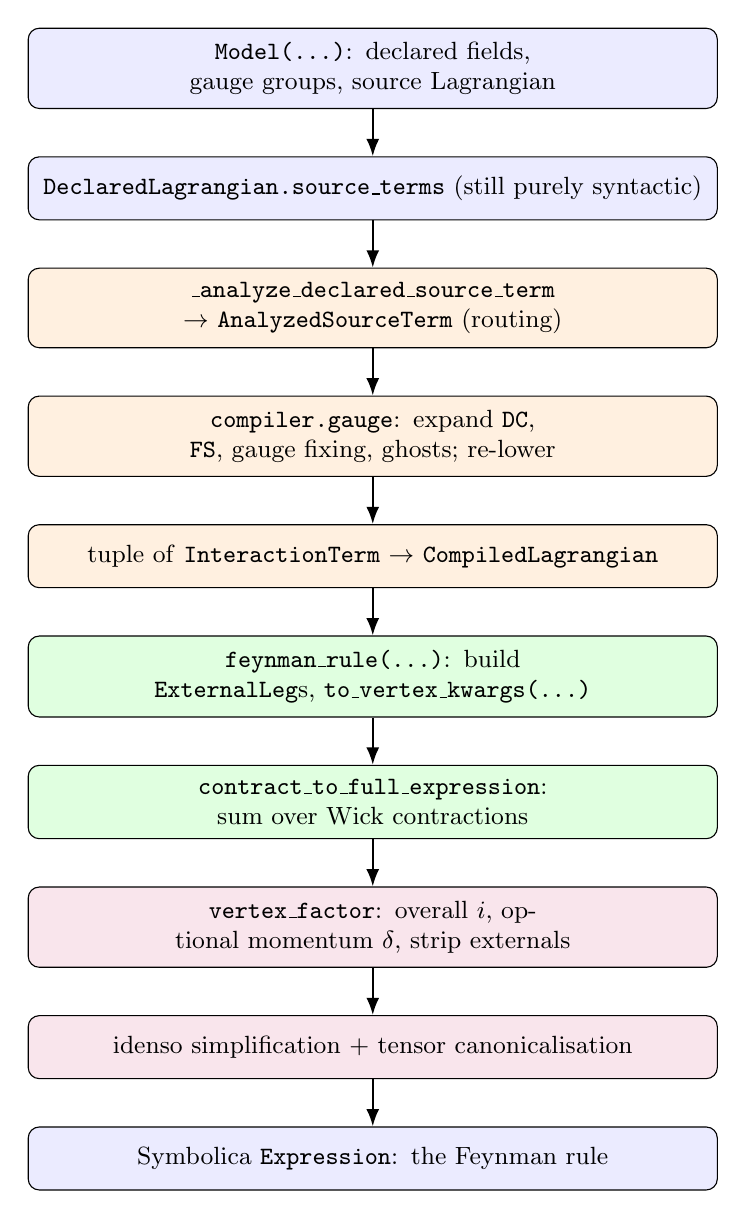
\begin{tikzpicture}[
    node distance=6mm,
    box/.style={draw, rounded corners, align=center, text width=8.4cm,
                minimum height=8mm, font=\small, inner sep=5pt},
    decl/.style={box, fill=blue!8},
    comp/.style={box, fill=orange!12},
    eng/.style={box, fill=green!12},
    post/.style={box, fill=purple!10},
    arr/.style={-{Latex[length=2.2mm]}, thick}
]

\node[decl]                      (model)     {\texttt{Model(...)}: declared fields, gauge groups, source Lagrangian};
\node[decl,  below=of model]     (declared)  {\texttt{DeclaredLagrangian.source\_terms} (still purely syntactic)};
\node[comp,  below=of declared]  (analyze)   {\texttt{\_analyze\_declared\_source\_term} $\to$ \texttt{AnalyzedSourceTerm} (routing)};
\node[comp,  below=of analyze]   (compile)   {\texttt{compiler.gauge}: expand \texttt{DC}, \texttt{FS}, gauge fixing, ghosts; re-lower};
\node[comp,  below=of compile]   (terms)     {tuple of \texttt{InteractionTerm} $\to$ \texttt{CompiledLagrangian}};
\node[eng,   below=of terms]     (legs)      {\texttt{feynman\_rule(...)}: build \texttt{ExternalLeg}s, \texttt{to\_vertex\_kwargs(...)}};
\node[eng,   below=of legs]      (contract)  {\texttt{contract\_to\_full\_expression}: sum over Wick contractions};
\node[post,  below=of contract]  (factor)    {\texttt{vertex\_factor}: overall $i$, optional momentum $\delta$, strip externals};
\node[post,  below=of factor]    (canon)     {idenso simplification + tensor canonicalisation};
\node[decl,  below=of canon]     (out)       {Symbolica \texttt{Expression}: the Feynman rule};

\foreach \a/\b in {model/declared, declared/analyze, analyze/compile,
                   compile/terms, terms/legs, legs/contract,
                   contract/factor, factor/canon, canon/out}
  \draw[arr] (\a) -- (\b);
\end{tikzpicture}
\caption{The pipeline from a declared \texttt{Model} to a Feynman-rule \texttt{Expression}. Blue = declaration layer (\texttt{feynpy}); orange = lowering/compiler layer (\texttt{feynpy.lowering}, \texttt{compiler.gauge} and helpers); green = contraction engine (\texttt{symbolic.vertex\_engine}); purple = post-processing (\texttt{symbolic.vertex\_postprocessing}, \texttt{symbolic.tensor\_canonicalization}).}
\label{fig:pipeline-overview}
\end{figure}

\begin{table}[htbp]
\centering
\begin{tabular}{@{}p{2.6cm}p{3.6cm}p{6.8cm}@{}}
\toprule
\textbf{Layer} & \textbf{Package(s)} & \textbf{Responsibility} \\
\midrule
Declaration &
\texttt{feynpy} (\texttt{metadata}, \texttt{declared}, \texttt{core}) &
Represents the physics as the user wrote it: declared fields, gauge groups, and source Lagrangian terms, still in a mostly syntactic form. \\
Lowering \& compilation &
\texttt{feynpy.lowering}, \texttt{lagrangian}, \texttt{compiler} &
Classifies and validates each source term, expands gauge structures such as covariant derivatives, field strengths, gauge-fixing terms and ghosts into local monomials, and collects the result into \texttt{InteractionTerm}s. \\
Contraction engine &
\texttt{symbolic.vertex\_engine} &
Builds external legs and vertex arguments, then sums over Wick contractions to assemble the full expression. \\
Post-processing &
\texttt{symbolic.vertex\_postprocessing}, \texttt{symbolic.tensor\_canonicalization} &
Applies the overall factor of $i$, optionally extracts the momentum-conserving $\delta$, strips external-leg factors, and simplifies and canonicalises the resulting tensor expression. \\
\bottomrule
\end{tabular}
\caption{The four layers of the pipeline, coloured as in Figure~\ref{fig:pipeline-overview}: declaration (blue), lowering/compilation (orange), contraction (green), and post-processing (purple).}
\label{tab:internals-layers}
\end{table}

The remaining sections walk the layers from the outside in: declaration (Section~\ref{sec:internals-declaration}), analysis and index resolution (Section~\ref{sec:internals-lowering}), gauge compilation (Section~\ref{sec:internals-compiler}), the \py{InteractionTerm} intermediate representation that ties everything together (Section~\ref{sec:internals-ir}), the Wick-contraction engine (Section~\ref{sec:internals-contraction}), and canonicalisation (Section~\ref{sec:internals-postprocessing}). Section~\ref{sec:internals-difficulty} then collects the hardest problems encountered while building the pipeline --- the places where the design had to be most deliberate.

\footnote{Each TikZ figure in this chapter has a plain-text counterpart kept as a Mermaid source diagram under \texttt{viz/mermaid/}}

% --------------------------------------------------------------
\section{The outer layer: declaring a model}
\label{sec:internals-declaration}
% --------------------------------------------------------------

\subsection{Inert metadata}

In the chapter \ref{ch:feynpy} we have seen all the building blocks of FEYNPY that will enable us to define the Model. These building blocks are the declarative \emph{metadata} stored in \texttt{feynpy.metadata}; these are frozen dataclasses that hold physics data and carry no algorithmic logic. Let's summarise them here:
\begin{itemize}
    \item \py{IndexType} pairs a Spenso representation with a ``kind'' string and a label prefix (more in Section~\ref{sec:cas-indextype});
    \item \py{Field} stores a name, spin, self-conjugacy, its tuple of \py{indices}, its Symbolica symbol and conjugate symbol, quantum numbers, and optional flavour-class data, inferring its \py{kind} (scalar/fermion/vector) and \py{statistics} from the spin;
    \item \py{Parameter} behaves algebraically like its symbol and may carry indices and explicit components;
    \item \py{GaugeRepresentation} and
    \item \py{GaugeGroup} record the symmetry data, whether a group is abelian, its coupling, gauge boson, ghost field, structure-constant builder and matter representations
\end{itemize}

The deliberate point is that metadata is inert: a faithful, machine-readable copy of what a physicist would write on paper, with all behaviour deferred downstream.

\subsection{The declarative DSL as wrapper objects}

Now that we have defined the building blocks of the theory, we can put them together into the Lagrangian itself. This is done with a small domain-specific language (DSL) defined in \texttt{feynpy.declared}:\footnote{A domain-specific language is a small language designed for a particular task. Here it is a restricted set of Python objects and functions that lets the user write Lagrangian terms in a notation close to standard physics notation.} \py{DC} (covariant derivative), \py{FS} (field strength), \py{Gamma}, \py{PartialD}, \py{Metric}, \py{T}, \py{StructureConstant}, \py{GaugeFixing}, \py{GhostLagrangian}. I want to emphasise that these constructors do not immediately build a Symbolica tensor expression. They build small immutable wrapper objects that will later be analysed and lowered into compiled interaction terms.

To understand how the code reads the Lagrangian let's consider as an example the equation \ref{eq:qcd-full}. When the user writes the equation \ref{eq:qcd-full} the first term looks like this
\begin{minted}{python}
I * Quark.bar * Gamma(mu) * DC(Quark, mu)
\end{minted}

Obviously the Lagrangian in equation \ref{eq:qcd-full} is composed of many terms, and so the first thing the code needs to do is to distinguish each monomial and separate its scalar coefficient from its field and tensor factors. More precisely the code assembles a \py{_DeclaredMonomial} which distinguishes between the coefficient and an ordered tuple composed of all the other factors. In our case its content is simply a scalar coefficient (\py{I}) and an ordered tuple that stores every factor --- here \py{_FieldFactor(Quark, conjugated=True)}, \py{GammaFactor(mu)}, \py{CovariantDerivativeFactor(Quark, mu)}. At this stage nothing is contracted, expanded or simplified. The order of the factors is preserved exactly because later passes need the original source structure. Later a process of analysis will determine what needs to be expanded.

A useful subtlety is that a few helpers are \emph{dual}. \py{Gamma(mu)} and \py{T(a)} are declarative placeholders: they say ``insert the gamma matrix'' or ``insert the generator'' and let the lowering pass infer the endpoints from the neighbouring fields. By contrast, \py{Gamma(i, j, mu)} and \py{T(a, i, j)} bypass that shorthand and return the fully explicit Spenso tensors \py{gamma(i, j, mu)} and \py{t(a, i, j)} immediately. This gives the user both a compact notation without specifying every index explicitly when the structure is obvious, and a fully explicit notation when it is not.

\subsection{\texttt{Model} and the two Lagrangian containers}

Once individual source terms have been written, the full source Lagrangian is stored in the container \py{DeclaredLagrangian}. This is a very simple object: essentially it is just an ordered tuple \py{source_terms}. In the most common case these source terms are \py{_DeclaredMonomial}s, but they can also be special declarations such as \py{GaugeFixing(...)} or \py{GhostLagrangian(...)}. So \py{DeclaredLagrangian} is nothing but the source-level Lagrangian, still written in the declarative language.

Everything is put together in the \py{Model} (in \texttt{feynpy.core}); this is the larger object that owns this declared Lagrangian together with the rest of the model data: \py{fields}, \py{parameters} and \py{gauge_groups}. Now the input is converted into a \py{DeclaredLagrangian}.

Actual compilation happens only when \py{model.lagrangian()} is called. At that point the declared source terms are turned into a \py{CompiledLagrangian}. This is where terms containing \py{DC(...)} or \py{FS(...)} are expanded using the metadata stored in the model, while terms that are already local are lowered directly. The result is no longer source syntax: it is a tuple of compiled \py{InteractionTerm}s. This compilation is lazy and cached, so it is only done the first time it is needed.

To summarise: \py{DeclaredLagrangian} is the source-level Lagrangian, \py{CompiledLagrangian} is the compiled one, and \py{Model} is the full object that stores the declared Lagrangian together with the extra information needed to validate and compile it.

% --------------------------------------------------------------
\section{Analysis and lowering: reading the Lagrangian and resolving indices}
\label{sec:internals-lowering}
% --------------------------------------------------------------

Between \py{DeclaredLagrangian} and \py{CompiledLagrangian} there is an intermediate step. The declared Lagrangian is the user-written Lagrangian, while the compiled Lagrangian is a tuple of local \py{InteractionTerm}s. Therefore we first need to make every implicit structure explicit, validate its index labels, and decide whether this term needs a model-dependent expansion. This process is what we call lowering.

For example, consider again the declared quark kinetic term
\begin{minted}{python}
I * Quark.bar * Gamma(mu) * DC(Quark, mu)
\end{minted}
Lowering checks that \py{mu} is used consistently as a Lorentz index and that the implied spinor and colour structure is well-formed, and classifies the term as a \py{covariant_core}. This still is not a final local interaction term, because \py{DC} must first be expanded using the model's gauge data. The compiler then performs that expansion, producing ordinary local monomials such as the kinetic piece and the quark--gauge-boson vertex, and those local monomials are what finally become compiled \py{InteractionTerm}s. By contrast, a source term that is already local, such as \py{lam * phi**4}, is lowered directly into its canonical interaction form with no further expansion.

So the lowering layer (\texttt{feynpy.lowering}) is the bridge between declarative syntax and the compiler. For each source term it answers three questions: what kind of term is this, are its indices well-formed, and (if the term is already local) what is its canonical interaction form?

\subsection{Classifying each source term}

In order to know what needs to be expanded, and how, by the compiler we want to analyse the terms. The single entry point is \py{_analyze_declared_source_term(...)}, which returns an \py{AnalyzedSourceTerm}. This object has the role of routing correctly every monomial through the compilation. If the term is already local, it already contains the final \py{InteractionTerm}; otherwise it stores the structured object that the compiler must expand. The compiler then consumes this analysed object, expanding it according to the gauge structure. The categories are summarised in Table~\ref{tab:analyzed-categories}.

\begin{table}[htbp]
\centering
\begin{tabular}{@{}p{4.0cm}p{5.0cm}p{3.2cm}@{}}
\toprule
\textbf{Category} & \textbf{Meaning} & \textbf{Example} \\
\midrule
\texttt{interaction} & a local \py{InteractionTerm}; no compilation & \py{lam * phi**4} \\
\texttt{covariant\_core} & canonical kinetic $\bar\psi\, i\gamma^\mu D_\mu \psi$ or $(D_\mu\Phi)^\dagger(D^\mu\Phi)$ & quark kinetic term \\
\texttt{generic\_covariant\_monomial} & any other monomial that still contains \py{DC} or another covariant operator needing expansion & current$\,\times\,$current \\
\texttt{gauge\_fixing} & a gauge-fixing declaration & \py{GaugeFixing(SU3, xi)} \\
\texttt{ghost} & a ghost declaration & \py{GhostLagrangian(SU3)} \\
\texttt{field\_strength\_monomial} & a monomial built from \py{FS(...)} factors & $-\tfrac14 F^a F^a$ \\
\bottomrule
\end{tabular}
\caption{The classification produced by \texttt{\_analyze\_declared\_source\_term}}
\label{tab:analyzed-categories}
\end{table}

So the analyser asks whether the term is already local; if not it proceeds with the classification. It checks if it is one of the two covariant kinetic shapes, afterwards if it is a generic covariant operator, which is a mix of covariant derivative, field strength and fields. There is also a dedicated classification for the gauge-fixing and ghost declarations (used in the declarative helper), and finally pure field-strength monomials.

\subsection{Resolving the indices}

As explained earlier, we do not want the user to have to write out every index in the Lagrangians, as many are implicit and obvious to a physicist. In this `lowering' stage, terms with implicit index structure are made explicit. The lowering process determines which symbolic labels belong to which field slots and which contractions the user intended to apply. A large amount of the design effort has been devoted to this stage, as it is precisely here that silent errors are most dangerous.


\paragraph{Monomial-wide label validation.} A first validation before lowering is done. The analyser builds one registry for every label \emph{name} appearing anywhere in the monomial (on field slots, on \py{PartialD}, \py{Gamma}, \py{T}, $f^{abc}$ and \py{FS}, and even on raw Spenso tensors in the coefficient) and requires that each name correspond to exactly one \py{IndexType}. Meaning that if the analyser encounters a label \py{f} as a flavour index it cannot appear on another field in the monomial as an adjoint index for example. So if the same name is used for two incompatible kinds the term is rejected with an explicit error.


\paragraph{Slot binding and inference.} Once each symbolic label has been assigned an index type (for example Lorentz, spinor, colour or flavour) the local monomial is resolved in a predefined order. Firstly, all labels that the user has entered directly into the fields are retained. Next, factors such as \py{Gamma} and \py{T}, which sit between two neighbouring fields, are resolved by identifying which field slots they connect to, to understand how to contract. Lowering replaces them by the corresponding explicit Spenso tensor, represented as a Symbolica expression, and multiplies that tensor into the coupling. Next, any other explicit labels --- such as those from declared factors or tensors already present in the coefficient --- are matched to the remaining free field slots of the same type. This matching must be one-to-one; if multiple assignments are possible, the lowering process generates an ambiguity error. After all explicit information has been used, the process proceeds to default assignment: it assigns new labels to obvious pairs, such as an adjacent $\bar\psi/\psi$, then to the sole remaining compatible pair, and finally introduces new dummy labels for any slots still left open. The result is that a compact source monomial is transformed into a fully explicit indexed interaction term, or rejected with a clear error if the notation is genuinely ambiguous.



\subsection{Remembering fermion pairings}

During lowering, the code records one further piece of information: how the fermion factors are paired into closed Dirac bilinears. This information is stored in the \py{closed_dirac_bilinears} metadata, a list of $(\bar\psi\text{-slot},\,\psi\text{-slot})$ pairs. The code determines these pairings automatically from the local spinor structure of the term.

This step is deliberately conservative. Lowering keeps this metadata only when the fermion slots can be partitioned unambiguously into disjoint, ordered closed bilinears. If no unique pairing is found, the monomial is rejected rather than guessed. When the pairing is unambiguous, the metadata preserves which \(\bar\psi\) is paired with which \(\psi\), so that the contraction engine can later apply the correct fermion-sign convention. Its importance is discussed in Section~\ref{sec:internals-difficulty}.

% --------------------------------------------------------------
\section{Compilation: turning gauge structure into ordinary interactions}
\label{sec:internals-compiler}
% --------------------------------------------------------------

Now the phase of full expansion of every operator of the Lagrangian is done. The compiler stage is the first stage that needs all the information stored in the model concerning the gauge symmetries. Through the lowering stage we analysed the terms and now with the compilation we turn the remaining unexpanded object into a local interaction term. The main dispatch lives in \texttt{src/compiler/gauge.py}: \py{_compile_declared_lagrangian_terms(model)} walks the analysed source terms and sends each one to a specialised handler (Figure~\ref{fig:compiler-dispatch}). Throughout this stage the conventions are
\begin{equation}
    D_\mu = \partial_\mu - i g\, A_\mu^a T_a,
    \qquad
    F_{\mu\nu} = \frac{i}{g}[D_\mu,D_\nu]
    = F^a_{\mu\nu} T_a ,
    \label{eq:conventions}
\end{equation}
with the adjoint basis fixed by
\begin{equation}
    [T_b,T_c] = i\, c^{a}{}_{bc}\, T_a,
    \qquad
    F^a_{\mu\nu}
    = \partial_\mu A^a_\nu - \partial_\nu A^a_\mu + g\, c^{a}{}_{bc}\, A^b_\mu A^c_\nu .
    \label{eq:conventions-components}
\end{equation}
For the usual \(\mathrm{SU}(N)\) basis one may simply read \(c^{a}{}_{bc}\) as the familiar \(f^{abc}\). Extra invariant tensors of the group, such as \(\epsilon\)-tensors or symmetric \(d\)-symbols, can certainly appear in local operators and coefficients, but they do not modify the definitions of \(D_\mu\) or \(F_{\mu\nu}\).

\begin{figure}[htbp]
\centering
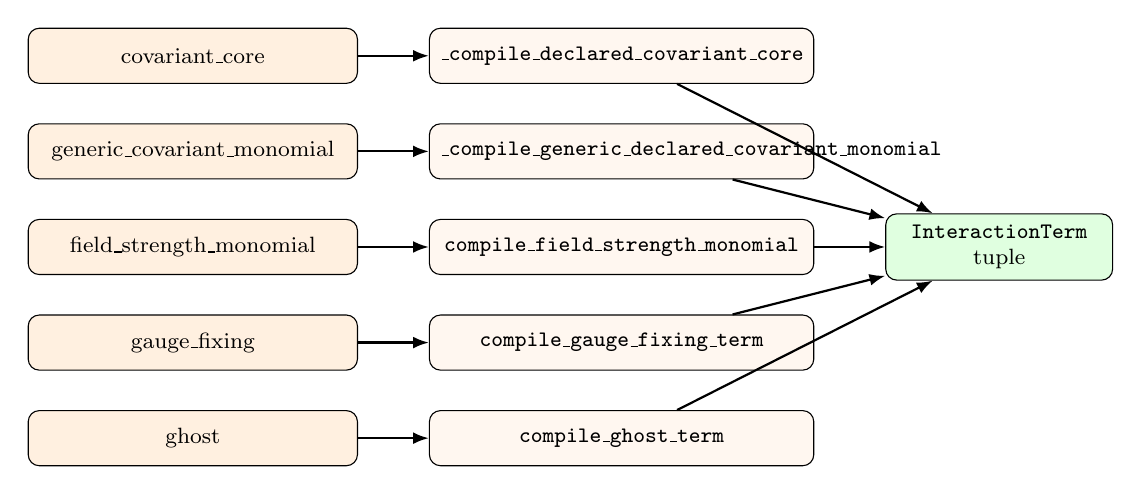
\begin{tikzpicture}[
    node distance=5mm and 9mm,
    box/.style={draw, rounded corners, align=center, font=\footnotesize,
                inner sep=4pt, minimum height=7mm},
    comp/.style={box, fill=orange!12, text width=3.9cm},
    hand/.style={box, fill=orange!6, text width=4.6cm},
    ir/.style={box, fill=green!12, text width=2.6cm},
    arr/.style={-{Latex[length=2mm]}, thick}
]
\node[comp] (c1) {covariant\_core};
\node[comp, below=of c1] (c2) {generic\_covariant\_monomial};
\node[comp, below=of c2] (c3) {field\_strength\_monomial};
\node[comp, below=of c3] (c4) {gauge\_fixing};
\node[comp, below=of c4] (c5) {ghost};

\node[hand, right=of c1] (h1) {\texttt{\_compile\_declared\_covariant\_core}};
\node[hand, right=of c2] (h2) {\texttt{\_compile\_generic\_declared\_covariant\_monomial}};
\node[hand, right=of c3] (h3) {\texttt{compile\_field\_strength\_monomial}};
\node[hand, right=of c4] (h4) {\texttt{compile\_gauge\_fixing\_term}};
\node[hand, right=of c5] (h5) {\texttt{compile\_ghost\_term}};

\node[ir, right=of h3] (ir) {\texttt{InteractionTerm} tuple};

\foreach \c/\h in {c1/h1, c2/h2, c3/h3, c4/h4, c5/h5} \draw[arr] (\c) -- (\h);
\foreach \h in {h1, h2, h3, h4, h5} \draw[arr] (\h) -- (ir);
\end{tikzpicture}
\caption{Compiler dispatch. Each analysed category is handled by one routine, and every routine returns ordinary \texttt{InteractionTerm} objects. Structured operators are first expanded into local monomials and then lowered through the same path as hand-written interactions.}
\label{fig:compiler-dispatch}
\end{figure}

\subsection{Expansion and Interaction Term building}

The compiler essentially performs two operations. Firstly, it expands each structured gauge operator to yield simple local monomials. Secondly, only after carrying out the complete expansion does it feed these monomials back into the normal lowering process, generating a \py{InteractionTerm} (Section~\ref{sec:internals-lowering}).

This is a deliberate design choice: it prioritises generality and a single, uniform compilation pipeline over efficiency. For example dedicated routines could be written for $F^2$, $F^3$, $F^4$ and for each covariant structure separately, which would make it faster and more importantly closer to the canonical form we already know from textbooks. Here, however, there is no separate, hard-coded compiler for $F^2$, $F^3$, $F^4$ or for every possible power of a covariant derivative. The combinations are generated automatically via the standard distribution followed by a well-established lowering phase.

The cost is that the intermediate output is much more verbose than textbook notation. A non-abelian $F^2$ expands into nine local monomials before canonicalisation combines equivalent terms again (Section~\ref{sec:internals-postprocessing}). For higher operators this growth is rapid; for pure non-abelian $F^n$ it gives $3^n$ branches. Much of the effort has therefore gone into the canonicalisation process.

\subsection{Covariant derivatives}
\label{sec:internals-covd}

Let us examine the expansion of the covariant derivative in more detail. For a field $\phi$ transforming under several gauge groups, we define the general covariant derivative as

\begin{equation}
    D_\mu \phi
    =
    \partial_\mu \phi
    -
    i \sum_G g_G A^{a_G}_{G,\mu}\,
    \rho_G\!\left(T^{a_G}_G\right)\phi,
    \label{eq:covd-general}
\end{equation}

where the sum runs over all gauge groups $G$ under which $\phi$ transforms. Here, $T^{a_G}_G$ is a generator of $G$, while

\begin{equation}
    \rho_G : \mathfrak{g}_G \longrightarrow \operatorname{End}(V_G)
\end{equation}

is the representation map acting on the corresponding representation slot of $\phi$.

The two relevant cases are:

\begin{itemize}
    \item \textbf{Abelian group.} There is a single generator, represented by the charge $Q_G$. Therefore,
    \begin{equation}
        D_\mu \phi
        \supset
        -i g_G Q_G A^{(G)}_\mu \phi.
    \end{equation}

    \item \textbf{Non-abelian group.} The gauge field carries an adjoint index $a$, and the corresponding generator acts on the appropriate representation index of the field:
    \begin{equation}
        (D_\mu \phi)_i
        \supset
        -i g_G A^a_{G,\mu}
        \left(t^a_{G,R}\right)_{ij}\phi_j.
    \end{equation}
\end{itemize}

Let's take as an example a field that carries representation indices associated with several gauge groups, each generator acts only on its corresponding index. For example, for a field $\phi_{i\alpha}$ transforming in the tensor-product representation $R_1 \otimes R_2$,

\begin{equation}
    D_\mu \phi_{i\alpha}
    =
    \partial_\mu \phi_{i\alpha}
    -
    i g_1 A^a_\mu
    \left(t^a_{R_1}\right)_{ij}
    \phi_{j\alpha}
    -
    i g_2 B^b_\mu
    \left(t^b_{R_2}\right)_{\alpha\beta}
    \phi_{i\beta}.
\end{equation}

The routine \py{expand_cov_der} implements Eq.~\eqref{eq:covd-general} literally. It always emits one partial-derivative piece. It then resolves which gauge groups act on the field and emits one gauge piece for each of them; if the user did not name a group, it uses all compatible groups. For a conjugated occurrence $(D_\mu\phi)^\dagger$, the sign of the gauge piece flips.

\paragraph{More slots in the same representation.} The user might want to play with multiple slots in many representations that could be the same, in which case the generator may be able to act on more than one place. The code handles these cases. The default policy for this situation is conservative and rejects it as ambiguous.
 A representation can instead opt into \py{slot_policy='sum'}, in which case the compiler sums over the possible active slots.

\paragraph{Several gauge groups at once.} A standard example is the left-handed quark doublet $Q_L$, which transforms under $\mathrm{SU}(3)_c\times\mathrm{SU}(2)_L\times\mathrm{U}(1)_Y$. In that case
\begin{equation}
    D_\mu Q_L
    = \partial_\mu Q_L
    \;-\; i g_s\, G^a_\mu\, t^a_{(3)}\,Q_L
    \;-\; i g\, W^I_\mu\, t^I_{(2)}\,Q_L
    \;-\; i g'\, Y_{Q}\, B_\mu\, Q_L ,
    \label{eq:covd-multigroup}
\end{equation}
where we have $t^a_{(3)}$ as the colour generators, $t^I_{(2)}$ as the weak generators and $Y_Q$ as the hypercharge. So \py{DC(Q_L, mu)} expands to four pieces: the ordinary derivative plus one gauge current for each of the three groups. Naming one group, for example \py{DC(Q_L, mu, gauge_group=SU3C)}, keeps only that group's current together with the partial derivative.



\subsection{Field strengths}
\label{sec:internals-fs}

Let us examine the expansion of field strengths in more detail. As for the covariant derivative, the compiler expands \py{FS(...)} using the gauge-group data of the model so that it becomes a sum of local terms.

Using the convention

\begin{equation}
    D_\mu = \partial_\mu - i g A_\mu,
\end{equation}
with
\begin{equation}
    A_\mu = A_\mu^a T_a,
    \qquad
    [T_b,T_c] = i c^{a}{}_{bc} T_a,
\end{equation}
the Lie-algebra-valued field strength is
\begin{equation}
    F_{\mu\nu}
    =
    \partial_\mu A_\nu
    -
    \partial_\nu A_\mu
    -
    i g [A_\mu,A_\nu]
    =
    F^a_{\mu\nu}T_a,
\end{equation}
with components
\begin{equation}
    F^a_{\mu\nu}
    =
    \partial_\mu A^a_\nu
    -
    \partial_\nu A^a_\mu
    +
    g\,c^{a}{}_{bc}A^b_\mu A^c_\nu.
    \label{eq:fs-general}
\end{equation}


In the DSL, this is written as \py{FS(G, mu, nu, a)} for a non-abelian gauge group $G$, while for an abelian gauge group one writes \py{FS(G, mu, nu)}.

A single non-abelian \py{FS} factor is first rewritten as the sum
\begin{equation}
    F^a_{\mu\nu} = P_1 + P_2 + P_3,
\end{equation}
where
\begin{equation}
    P_1 = \partial_\mu A^a_\nu,
    \qquad
    P_2 = -\partial_\nu A^a_\mu,
    \qquad
    P_3 = g\,c^{a}{}_{bc}A^b_\mu A^c_\nu.
    \label{eq:fs-pieces}
\end{equation}
Note that for an abelian field strength, only $P_1$ and $P_2$ are present.

A monomial containing several field-strength factors is expanded by taking the full Cartesian product of all the different pieces.

To understand it more, let's consider the iconic example of the pure Yang--Mills Lagrangian
\begin{equation}
    \mathcal{L}_{\mathrm{YM}}
    =
    -\frac{1}{4}
    F^a_{\mu\nu}F^{a\,\mu\nu}.
\end{equation}
Each non-abelian field strength contributes three pieces, so their product generates
\begin{equation}
    3 \times 3 = 9
\end{equation}
raw branches before canonicalisation and collection. These branches belong to three sectors:
\begin{center}
\begin{tabular}{@{}lll@{}}
\toprule
\textbf{Piece combination} & \textbf{Count} & \textbf{Sector} \\
\midrule
$(P_1,P_2)\times(P_1,P_2)$
    & $2\times2=4$
    & quadratic kinetic sector \\
$(P_1,P_2)\times P_3$ and $P_3\times(P_1,P_2)$
    & $2+2=4$
    & cubic gauge interaction \\
$P_3\times P_3$
    & $1$
    & quartic gauge interaction \\
\bottomrule
\end{tabular}
\end{center}

Each resulting branch is then lowered in the same way as an ordinary local interaction.

Note that a product of $n$ non-abelian field strengths produces $3^n$ raw branches, whereas a product of $n$ abelian field strengths produces $2^n$ branches. More generally, a mixed product with $m$ non-abelian and $k$ abelian field strengths produces $3^m 2^k$ branches.



\subsection{Gauge fixing and ghosts}

There is a declarative helper for the gauge fixing term which can be accessed by \py{GaugeFixing(gauge_group, xi=...)}. This helper implements the linear covariant gauge term
\begin{equation}
    \mathcal{L}_{\mathrm{gf}}
    =
    -\frac{1}{2\xi}
    \left(\partial^\mu A^a_\mu\right)
    \left(\partial^\nu A^a_\nu\right),
\end{equation}
with the adjoint index omitted in the abelian case. It constructs the corresponding explicit local monomial, lowers it through the ordinary compilation pipeline, and tags the result as \py{gauge_fixing} so that the reporting and validation layers can recognise it. The user can naturally write the gauge fixing manually, in which case it is recognised and receives the same tag.

Note that the generic \py{GaugeFixing(...)} helper describes only linear covariant gauge fixing. More general $R_\xi$ gauges in spontaneously broken theories, for example, require additional Goldstone-dependent gauge-fixing terms, which must be written explicitly by the user.

There is also the ghost Lagrangian helper \py{GhostLagrangian(gauge_group)}. For a non-abelian gauge group, the Faddeev--Popov ghost Lagrangian can be written as
\begin{equation}
    \mathcal{L}_{\mathrm{gh}}
    =
    -\bar c^a\,
    \partial^\mu\left(D_\mu c\right)^a.
\end{equation}
Up to a total derivative, integration by parts gives
\begin{equation}
    \mathcal{L}_{\mathrm{gh}}
    \simeq
    \left(\partial^\mu\bar c^a\right)
    \left(D_\mu c\right)^a,
\end{equation}
where
\begin{equation}
    \left(D_\mu c\right)^a
    =
    \partial_\mu c^a
    +
    g\,c^{a}{}_{bc}A^b_\mu c^c.
\end{equation}
The ghost sector therefore becomes
\begin{equation}
    \mathcal{L}_{\mathrm{gh}}
    \simeq
    \left(\partial^\mu\bar c^a\right)
    \left(\partial_\mu c^a\right)
    +
    g\,c^{a}{}_{bc}
    \left(\partial^\mu\bar c^a\right)
    A^b_\mu c^c.
\end{equation}

The compiler turns the ghost sector into two ordinary local terms: the ghost kinetic term and the ghost gauge interaction term. Since the ghost field transforms in the adjoint representation, the code can use the same gauge-action and index-contraction machinery that it uses for other adjoint fields. What remains specific to ghosts is not the contraction structure, but their interpretation: they still carry Grassmann statistics, a fixed field ordering, and ghost number.

% --------------------------------------------------------------
\section{The pivot: the \texttt{InteractionTerm} intermediate representation}
\label{sec:internals-ir}
% --------------------------------------------------------------
To return to the analogy used at the start of the chapter, we are now at the waist of the hourglass. Every branch of the code converges and passes through this data type: \py{InteractionTerm} (in \texttt{feynpy.interactions}). Everything above this narrow point is declarative, everything below it is generic symbolic machinery.

\begin{minted}{python}
@dataclass(frozen=True)
class InteractionTerm:
    coupling: object                        # Symbolica Expression
    fields: tuple[FieldOccurrence, ...]     # bare field factors, in order
    derivatives: tuple[DerivativeAction, ...] = ()
    closed_dirac_bilinears: tuple[tuple[int, int], ...] = ()
    label: str = ""
    sector: str = ""
\end{minted}

The \py{coupling} is a Symbolica expression holding the numerical and tensor prefactor (couplings, generators, structure constants, metrics); \py{fields} is an ordered tuple of \py{FieldOccurrence} objects, each a field with its slot-resolved index labels and conjugation flag; \py{derivatives} records, as a \py{DerivativeAction}, which field each derivative hits and along which Lorentz index; and \py{closed_dirac_bilinears} carries the fermion-pairing provenance of Section~\ref{sec:internals-lowering}. A \py{CompiledLagrangian} is simply a tuple of such terms. An \py{InteractionTerm} is a purely static, index-labelled description of one monomial of the Lagrangian --- the direct code counterpart of the right-hand side
\[
    g_{\alpha_1\cdots\alpha_n}\,
    \partial\cdots\partial\,
    \phi^{\alpha_1}\cdots\phi^{\alpha_n}
\]
of Eq.~\eqref{eq:general-term}.

As we know the ordering of \py{fields} is relevant and since Symbolica multiplication is commutative, we use the ordered tuple which keeps record of fermion order.
The method \py{to_vertex_kwargs(external_legs)} performs the last model-aware step: it strips away all model-layer vocabulary and reduces one term plus a chosen set of external legs to flat, parallel lists --- species keys, momenta, field and leg roles, index labels and types, derivative indices and targets, and the bilinear metadata --- after which only Symbolica and Spenso objects remain.

\subsection*{Flavour expansion}

When the field carries a flavour index (Section~\ref{sec:feynpy-flavor}) by default the terms remain generic. For example $\lambda_{ij}\,\bar\ell_i \ell_j\,\phi$ will keep the lepton. By requesting \py{flavor_expand=True} FEYNPY enumerates every member combination, substitutes the corresponding \py{Parameter} component (e.g.\ $\lambda_{e\mu}$) producing one fully explicit \py{InteractionTerm} per combination in the same data structure.

\subsection*{Field transformations}
\label{sec:internals-transformations}

There is a second rewriting that lives at this layer, and it is the one that
produces the physical basis of the Standard Model. A
\py{FieldTransformation} (Section~\ref{sec:feynpy-transformations}) is applied
not to the declared source terms but to the compiled ones: each
\py{InteractionTerm} is visited, every \py{FieldOccurrence} matching a rule is
replaced by the corresponding expression, and the term is rebuilt.

Placing the stage here, rather than earlier, is a deliberate choice with two
consequences. First, \py{DC} and \py{FS} have already been expanded using the
gauge-group metadata of the original basis, which is the only basis in which
that metadata is meaningful --- $B_\mu$ has a hypercharge, the photon does
not. Second, because the transformation operates on an \py{InteractionTerm},
it inherits the structure that the term carries: derivatives recorded in
\py{derivatives} are distributed over a replacement product by the Leibniz
rule automatically, conjugated occurrences receive the conjugated
replacement, and the ordering that fixes fermion signs is preserved. A rule
that maps one field to a sum simply multiplies the number of terms, and
canonicalisation collects them again afterwards.

The transformation stage runs once, with all rules acting simultaneously, so
that a field introduced by one rule is not consumed by another in the same
pass. The result is an ordinary \py{CompiledLagrangian}, indistinguishable in
type from the one that entered, and vertex extraction proceeds from it
unchanged.

% -----------------------------------------------------
\section{The inner core: Wick contraction in the vertex engine}
\label{sec:internals-contraction}
% --------------------------------------------------------------

Now we arrive at the heart of the code, where the actual algorithm is implemented. We find the implementation of Wick contraction in
the vertex engine (\texttt{symbolic.vertex\_engine}). The only thing this engine cares about are fields, roles, index labels, momenta and a coupling tensor, and performs a combinatorial contraction that is the code-level realisation of the canonical-quantisation algorithm of Section~\ref{sec:feynrules-algorithm}.

\subsection{The permutation sum}

The core routine is \py{contract_to_full_expression}. Given an interaction with $n$ field slots and $n$ external legs, it sums over all $n!$ ways of matching legs to slots. Each permutation \py{perm} assigns leg \py{perm[i]} to slot \py{i}; the sum of the surviving contributions is the full Wick contraction.

For each permutation the code does the following things in order. First it remaps every open index in the coupling to the corresponding external-leg label, this ensures that the coupling will actually match the permuted fields. Then it checks whether the pairing is physically allowed, this is done using \py{factor_leg_compatible}. When it happens that a slot and a leg disagree in species, spin, statistics or conjugation, the permutation is discarded at once. Surviving fermionic terms pick up a Grassmann sign from the fermion part of the permutation, unless the closed-bilinear exception of Section~\ref{sec:internals-contraction-fermions} applies. Then derivatives are turned into momenta because of the Fourier rule $\partial_\mu \to -i p_\mu$ (all momenta incoming), so each \py{DerivativeAction} contributes a factor $(-i)\,p^\mu$ with $p$ the momentum of the matched leg (meaning that it will carry the corresponding label). Finally each leg contributes its external wavefunction ($U$ for bosons, $UF/\overline{UF}$ for fermions) and a species Kronecker delta, repeated indices are contracted with the Spenso metric, and the contribution is multiplied by the plane wave $\exp(-i\,\Sigma p\!\cdot\!x)$ before being added to the total.

Bosonic vertices carry no extra signs; fermionic ones do. The structure of the loop is:

\begin{minted}{python}
for perm in permutations(range(n)):
    term = coupling_with_open_indices_remapped_along(perm)
    if not all(factor_leg_compatible(i, perm[i], ...) for i in range(n)):
        continue                       # prune impossible pairing
    if statistics == "fermion" and not use_closed_dirac_bilinear_signs:
        term *= fermion_sign(perm, fermion_slots)
    for mu, tgt in zip(derivative_indices, derivative_targets):
        term *= (-I) * pcomp(ps[perm[tgt]], mu)
    for i, j in enumerate(perm):
        term *= external_factor(role[i], alphas[i], betas[j], ps[j], ...)
    term *= plane_wave(sum_of_matched_momenta, x)
    total += term
\end{minted}

Note that nothing here depends on a particular index kind. An index is only a \py{(kind, label)} pair.

\subsection{Fermion signs and the closed-bilinear exception}
\label{sec:internals-contraction-fermions}

Getting fermion signs right was one of the trickier parts of the engine. The pipeline records the order of the fields from the very start, so that even this final layer still knows which sign to apply.

The default rule is simple: use the flat Grassmann sign of the fermion permutation. This works in general, but it fails for a product of closed Dirac bilinears. A concrete example is the identical-fermion current--current operator
\begin{equation}
    (\bar\psi\,\gamma^\mu\psi)\,(\bar\psi\,\gamma_\mu\psi).
\end{equation}
This operator has two Wick contractions: a \emph{direct} one, where each current stays intact, and a \emph{crossed} one, where the two currents exchange a fermion. The flat Grassmann rule predicts a relative sign of $\text{direct} - \text{crossed}$ between the two, but the correct sign, following the FeynRules convention, is $\text{direct} + \text{crossed}$.


The fix uses the fermion-pairing information recorded during lowering (Section~\ref{sec:internals-lowering}). If that information shows that every Dirac fermion slot belongs to exactly one closed bilinear, the engine drops the flat permutation sign and treats every pairing with a plus. In every other case (for example a generic open multi-fermion tensor) the flat Grassmann sign still applies.

\subsection{Output policy and universal factors}

There is a function, namely \py{vertex_factor}, that has the role of running the contraction and then applies a few presentation choices. By default it amputates the external wavefunctions $U$, $UF$ and $\overline{UF}$, so the user sees the bare vertex. Optionally, the user can choose to write \py{include_delta=True}, which gives the momentum-conservation factor $(2\pi)^d\,\delta(\Sigma p)$. In every case the result is finally multiplied by the overall $+i$ that every Feynman rule carries. These choices only decide how the answer is shown.

% --------------------------------------------------------------
\section{Making the answer canonical}
\label{sec:internals-postprocessing}
% --------------------------------------------------------------

The raw contracted expression is correct, but not unique. The same vertex can appear with different dummy-index names, different orderings of antisymmetric tensors, or still expanded into many field-strength pieces. In the next paragraph some choices of the postprocessing of the final output are presented.

The first pass, in \texttt{symbolic.vertex\_postprocessing}, does the physics-facing clean-up. As the output comes out of the contraction engine it has the full range of Kronecker deltas of the permutation. The first step is therefore to contract species Kronecker deltas, collapse repeated bispinor indices with the Spenso metric, and, on request, simplify closed gamma chains with idenso (Section~\ref{sec:cas-idenso}).

The second pass, in \texttt{symbolic.tensor\_canonicalization}, puts the surviving expression into a unique tensor form using Symbolica's \py{canonize_tensors} (Section~\ref{sec:cas-symbolica}). That routine only understands symmetry flags on plain symbols, not on Spenso tensor heads. So the code temporarily replaces every Spenso tensor --- metrics, generators, structure constants, $\gamma$ matrices, and the project's custom invariants --- by a plain symbol with the right symmetry, runs the canonicalisation, and swaps the Spenso tensors back. Dummy indices of different kinds (Lorentz, colour, spinor, weak) are kept in separate groups, so a Lorentz dummy is never confused with a colour one.

On top of this, \py{canonize_full} adds a few physics reductions used when checking identities such as gauge variation and BRST (Sections~\ref{sec:feynpy-gauge-variation} and~\ref{sec:feynpy-brst}): it makes flat derivatives commute, reduces products of structure constants with the Jacobi identity, and drops Yang--Mills terms that vanish by the antisymmetry of $f^{abc}$.

Together these passes turn the over-expanded compiler output into a compact, comparable Feynman rule.

% --------------------------------------------------------------
\section{Where the difficulty lived}
\label{sec:internals-difficulty}
% --------------------------------------------------------------

Building the pipeline was less about one clever algorithm than about a few recurring hard problems. These are the places where most of the design effort went, and they shaped the architecture.

\paragraph{Index bookkeeping.} The hardest bugs came from indices, not from algebra. Early code keyed labels only by index kind, which fails as soon as a field carries two slots of the same kind --- two Lorentz indices, or two colour indices. The fix is now layered: labels are packed by slot, each label name is bound to one index type across the whole monomial, ambiguous assignments are rejected rather than guessed, and gauge representations expose an explicit \py{slot_policy}. The guiding rule is to fail early: an ambiguous index assignment is an error at declaration time, never a silent wrong contraction.

\paragraph{Fermion signs.} Matching the FeynRules convention for products of closed Dirac bilinears, without breaking generic multi-fermion terms, required carrying the bilinear pairing from lowering all the way into the contraction engine (Section~\ref{sec:internals-contraction-fermions}). Getting that boundary right --- all pluses only when every fermion sits in a closed pair --- took careful checks on benchmark operators and is now a fixed convention.



\paragraph{Making expansion generic.} Replacing a special-case $F^2$ handler with a generic \py{FS} expansion --- and likewise for covariant derivatives --- unlocked $F^3$, $F^4$ and mixed-group operators for free. The cost was many more raw local monomials, and a performance problem in the contraction engine: the old compatibility check compared only broad field roles and therefore tried many impossible pairings. The species-aware pruning of Section~\ref{sec:internals-contraction} fixed that without changing any resulting formula.

\paragraph{Keeping the layers honest.} Finally, much of the work went into not letting the layers leak into each other: declarative syntax must never reach the contraction engine, the engine must never know what a covariant derivative is, and comparison against external references must live outside the engine. One job per layer, and one intermediate representation at the waist, is what made it possible to validate the packaged Standard Model against the reference export vertex by vertex.

% --------------------------------------------------------------
\section{Summary}
\label{sec:internals-summary}
% --------------------------------------------------------------

The pipeline is a chain of small, inspectable rewrites. A \py{Model} holds the source Lagrangian and the inert data of the theory. Lowering classifies each term, checks its indices, and turns local terms into \py{InteractionTerm}s. The compiler expands gauge structure --- covariant derivatives, field strengths, gauge fixing and ghosts --- into ordinary local monomials and lowers them through the same path. Every branch therefore meets at the same intermediate representation. The symbolic engine then contracts it by a pruned permutation sum, applies momenta, external factors, fermion signs and the overall $+i$, and canonicalisation makes the answer unique. The hard parts --- indices, fermion signs, conventions, generic expansion and layer boundaries --- are exactly where the design had to be most careful, and they are what the validation in the next chapter rests on.

% ============================================================
%  07_validation.tex -- Validation and final comparison
% ============================================================

\chapter{Validation and Final Comparison}
\label{ch:validation}

Chapter~\ref{ch:internals} described how FeynPy turns a declared Lagrangian
into a Feynman-rule \texttt{Expression}. This chapter checks that output
against an independent reference: the FeynRules exports of the same models.
FeynRules is treated as the mathematical oracle throughout.

The two outputs are not expected to be \emph{identical} as printed
expressions. FeynRules and FeynPy package charge conjugation differently,
expand covariant derivatives to different depths, and represent chirality
differently (an explicit projector in FeynRules, a field class in FeynPy).
What is checked instead is that the two outputs are \emph{equal as tensors}:
that they differ only by index relabelling, reordering of commuting factors,
and a small, explicitly listed set of gauge and Lorentz identities. Section
\ref{sec:validation-canonical} makes this precise and shows, with two worked
examples, what that equality test actually does.

The headline results: the packaged Standard Model matches its FeynRules
export exactly ($163/163$ vertices), the unbroken background-field Standard
Model matches its own export exactly ($67/67$), and the SMEFT2 Green-basis
model matches all $184$ exported rows of the FeynRules EFT-only
\texttt{Ltot}. Of those $184$ SMEFT2 rows, $161$ match with no assumption at
all, $15$ match after one globally fixed charge-conjugation convention, and
$8$ match after an additional, explicitly tabulated row-specific transform.
No row is accepted by searching over signs or field orderings, and no row is
left unresolved.

% --------------------------------------------------------------
\section{Validation strategy}
\label{sec:validation-strategy}
% --------------------------------------------------------------

The validation has three layers, and they must not be conflated: the outer
two bound what the inner one can mean. A perfect equality score over a small,
cherry-picked subset of a model would prove very little.

\paragraph{Model fidelity.} Does the FeynPy source transcribe every operator
of the FeynRules source? A question about the \emph{input}, answered in
\Cref{sec:validation-fidelity} by a block-by-block and
coefficient-by-coefficient audit.

\paragraph{Vertex equality.} Do the Feynman rules derived from the two
Lagrangians agree as tensor expressions? The substance of the comparison,
answered in \Cref{sec:validation-canonical} and
\Cref{sec:validation-smeft2,sec:validation-ec}.

\paragraph{Coverage.} How much of the model does the equality test actually
reach? The FeynRules export covers a finite set of vertex arities, so some
operators may be structurally unreachable; see \Cref{sec:validation-coverage}.

Underneath all three sits an ordinary unit and regression suite for the
reusable engine: index validation, covariant expansion, field-strength
expansion, field transformations, fermion signs, tensor canonicalisation, and
selected benchmark Feynman rules.

Model-level comparisons live beside the concrete model packages under
\path{models/}, not inside the generic contraction engine: the engine
computes rules, and each model package owns the conventions and the
external-reference adapter needed to compare its own rules. The
format-independent comparison machinery itself is shared across models
(\Cref{sec:validation-generality}).

% --------------------------------------------------------------
\section{What ``equal'' means: the canonical form}
\label{sec:validation-canonical}
% --------------------------------------------------------------

Both sides of a comparison start as text: a FeynRules row is a
Mathematica-syntax string, such as \texttt{TensDot[Ga[mu],ProjM]}, and a
FeynPy row is produced by \texttt{feynman\_rule(...)} as described in
Chapter~\ref{ch:internals}. Both are parsed into Symbolica tensor
expressions before anything else happens; index brackets become index
symbols, \texttt{ProjM}/\texttt{ProjP} become chiral projectors, and indexed
Wilson parameters such as \texttt{alphaEcll[f1,f2,f3,f4]} become function
symbols \texttt{alphaEcll(f1,f2,f3,f4)}.

Two pieces of terminology are used throughout the rest of this chapter. The
\emph{signature} of a row is the ordered list of external field names, for
example \texttt{B|dR|dRbar} for the vertex coupling the hypercharge boson to
a right-handed down quark and its conjugate. The \emph{coefficient head} is
the name of the Wilson parameter multiplying a term, for example
\texttt{alphaEcll}. Comparison is always done per coefficient head within a
matching signature, never on a full undifferentiated sum (see below).

Equality is \emph{not} decided by comparing these parsed expressions
directly, nor by any string comparison. Two tensor expressions describing the
same physics can differ in ways that have nothing to do with whether the
physics is right: they can use different names for a summed-over (dummy)
index, write commuting factors in a different order, or leave the same
result differently expanded. Both sides are therefore reduced to a
\emph{canonical tensor-monomial map} --- a dictionary from canonical tensor
term to exact rational coefficient --- by
\path{src/symbolic/tensor_canonicalization.py}, and two rows are declared
equal exactly when their maps are identical, entry for entry, coefficient for
coefficient.

The reduction has four steps: (1) live tensor heads (the symbol names, e.g.\
the metric $g^{\mu\nu}$ or the Levi-Civita tensor $\epsilon^{\mu\nu\rho\sigma}$)
are swapped for temporary heads carrying explicit symmetry metadata, so the
canonicaliser is told which tensors are symmetric or antisymmetric under
index exchange; (2) Symbolica's tensor canonicaliser runs with contracted
dummy indices grouped, so their names carry no information; (3) dummy names
are standardised and commuting factors are sorted into one fixed order; (4)
the result is read off as the coefficient map.

\paragraph{Example 1: dummy names and symmetry.} The two expressions
\begin{equation}
    g^{\mu\nu}\, p_\mu k_\nu
    \qquad \text{and} \qquad
    g^{\nu\mu}\, k_\nu p_\mu
    \label{eq:validation-metric-example}
\end{equation}
are the same number for every $p,k$, but as raw Symbolica expressions they
differ in index naming ($\mu \leftrightarrow \nu$) and in the metric's index
order. Step (1) tells the canonicaliser that $g^{\mu\nu}=g^{\nu\mu}$; step (2)
identifies the two contracted-index pairs; only with both is the
canonicaliser able to reduce both expressions to the same map entry. Without
step (1), $g^{\mu\nu}$ and $g^{\nu\mu}$ would be treated as unrelated tensors
and the two expressions would wrongly be reported as different.

\paragraph{Example 2: generator reordering.} FeynRules and FeynPy can write
two colour or weak generators multiplying the same current in either order,
depending on the order in which the source Lagrangians introduced them. The
two orders are related by
\begin{equation}
    [T^a, T^b] = i f^{abc} T^c ,
    \label{eq:validation-commutator}
\end{equation}
so a term proportional to $T^b T^a$ on one side and $T^a T^b$ on the other
are equal only after adding the commutator term of
\Cref{eq:validation-commutator}. The canonicaliser applies exactly this one
identity when it encounters an out-of-order generator product
(\texttt{\_normalize\_generator\_product\_order\_report} in code); it does
not search over reorderings in general. The structure-constant Jacobi
identity,
\begin{equation}
    f^{abe}f^{cde} - f^{ace}f^{bde} + f^{ade}f^{bce} = 0 ,
    \label{eq:validation-jacobi}
\end{equation}
and the $SU(2)$ pseudoreality relations for $\epsilon_{ij}$ acting on a weak
generator are used the same narrow way, only where the two sides actually
need them.

These four steps and three identities are the entire simplification budget.
The comparison does \emph{not} use equations of motion, integration by parts,
momentum conservation, Schouten identities, Fierz identities, or any
open-ended pattern matching: admitting those would make the test far weaker,
because an incorrect rule could then often be massaged into the reference.

Two further design choices keep the comparison from degenerating into a
tautology. First, it runs \emph{separately for each coefficient head}: both
sides are filtered to the terms carrying a given head before the maps are
compared, so a cancellation between two different operators cannot mask an
error in either. Flavour order and complex conjugation stay inside the scalar
coefficient rather than being normalised away, so a term whose flavour
arguments have been silently transposed, e.g.\ $\alpha(f_2,f_1)$ for
$\alpha(f_1,f_2)$, is not judged equal merely because the coefficient head
name matches. Second, raw coefficient-head occurrence counts are recorded
only as a diagnostic, never as the equality criterion, because two equivalent
expanded forms can legitimately have different raw counts: FeynPy prints the
dual field strength $\mathrm{Dual}[F] = \tfrac{1}{2}\epsilon\cdot F$ as two
separate antisymmetric terms, where FeynRules has already used $\epsilon$
antisymmetry to collapse them into one. On the current SMEFT2 reference,
$100$ of $182$ shared signatures have matching raw counts, and every
remaining delta carries a recorded, specific reason; none is unexplained.

% --------------------------------------------------------------
\section{Standard Model benchmark}
\label{sec:validation-sm}
% --------------------------------------------------------------

The Standard Model package in \path{models/SM/} is the first complete
vertical slice of the project: a gauge-basis declaration, field
transformations to the physical basis, and a comparison of the resulting
interaction vertices against the bundled FeynRules \texttt{SM.fr} export.

The result is $163/163$ exact symbolic matches for the exported nonzero
flavour-expanded tree-level vertices, split by sector in
\Cref{tab:validation-sm-sectors}.

\begin{table}[htbp]
\centering
\begin{tabular}{lr}
\toprule
Sector & Vertices \\
\midrule
Gauge self-interactions & 8 \\
Matter currents & 51 \\
Yukawa & 42 \\
Higgs and Goldstone & 38 \\
Ghost & 24 \\
\midrule
Total & 163 \\
\bottomrule
\end{tabular}
\caption{Sector split of the Standard Model FeynRules comparison. Every row
in every sector is a direct exact symbolic match.}
\label{tab:validation-sm-sectors}
\end{table}

The scope should be stated precisely: the comparison runs with ghosts
included and gauge fixing disabled, so it validates the gauge, matter,
Yukawa, Higgs/Goldstone and ghost sectors but \emph{not} the gauge-fixing
sector, and it makes no claim about parameter-card semantics, loop-level
output, restriction files, or external formats such as UFO.

A second, independent benchmark is the unbroken background-field Standard
Model in \path{models/UnbrokenSM_BFM/}, matching its own FeynRules reference
at $67/67$ ($42$ three-point and $25$ four-point vertices). This matters for
SMEFT2, which is formulated in the same unbroken basis: it shows that the
basis, field naming, and generator conventions are already validated
independently of the EFT operators.

% --------------------------------------------------------------
\section{SMEFT2: model fidelity}
\label{sec:validation-fidelity}
% --------------------------------------------------------------

The main validation target is the SMEFT2 Green-basis model in
\path{models/SMEFT2/SMEFT2.py}, compared against the EFT-only FeynRules
\texttt{Ltot} export at
\path{models/SMEFT2/reference/Ltot_SMEFT_FeynRules.json}. The local FeynPy
\texttt{Ltot} follows the same convention, EFT contribution only, with the
SM-plus-EFT combination available separately as \texttt{Lfull}.

Before any vertex is compared, the transcription itself was audited. All
$32$ EFT Lagrangian blocks of \texttt{SMEFT\_Green\_Bpreserving.fr} are
implemented, and \texttt{Ltot} is composed from exactly those $32$ blocks in
the same order. All $298$ active Wilson coefficients of the FeynRules source
are declared in the FeynPy model and used in at least one operator; two
further coefficients, \texttt{alphaEcdlq} and \texttt{alphaEcqeu}, appear in
the FeynRules file but not in FeynPy, and both are commented out in
FeynRules and used in no FeynRules operator, so omitting them is correct
rather than a gap. (This is a statement about transcription, not about
comparison coverage: of the $298$ declared coefficients, the vertex
comparison of \Cref{sec:validation-smeft2} reaches $295$, for the structural
reason given in \Cref{sec:validation-coverage}.) The Standard Model core is
taken from \texttt{UnbrokenSM\_BFM.fr} minus its background-field ghost and
gauge-fixing sectors, deliberately excluded because the comparison target is
the EFT-only \texttt{Ltot}.

The structural differences between the two sources are systematic
conventions, not per-operator adjustments, as summarised in
\Cref{tab:validation-conventions}. This matters for
\Cref{sec:validation-ec}: because the FeynPy Lagrangian contains no
per-operator hand-fitting, a residual disagreement is evidence of a
\emph{convention} difference rather than of a transcription error.

\begin{table}[htbp]
\centering
\begin{tabular}{lll}
\toprule
FeynRules & FeynPy & Nature \\
\midrule
\texttt{2 Ta[...]} & \texttt{weak\_t} & named constant, 62 uses \\
\texttt{sigmamunu} & \texttt{sigma\_term} & named helper, 38 uses \\
\texttt{Dual[FS]} & \texttt{\_dual\_fs} & named helper \\
\texttt{lag + HC[lag]} & explicit \texttt{.conj()} terms & expansion \\
\texttt{CC[...]} & \texttt{dirac\_charge\_conjugation} & expansion \\
\bottomrule
\end{tabular}
\caption{Systematic convention differences between the FeynRules source and
the FeynPy transcription. No comparison-tuning comments, fudge factors, or
per-operator sign corrections appear in the model file.}
\label{tab:validation-conventions}
\end{table}

% --------------------------------------------------------------
\section{SMEFT2: comparison result}
\label{sec:validation-smeft2}
% --------------------------------------------------------------

All Green-basis and evanescent sectors used by the bundled reference are
included in the compiled FeynPy \texttt{Ltot}. The final result is given in
\Cref{tab:smeft2-final-comparison}; per-row verdicts are tabulated in
\Cref{app:smeft2-rows}.

\begin{table}[htbp]
\centering
\begin{tabular}{lr}
\toprule
Quantity & Result \\
\midrule
FeynRules reference rows & 184 \\
Operator-content matches & $184/184$ \\
\midrule
Direct exact symbolic matches & $161/184$ \\
Matches modulo the global \texttt{Ec} convention & $15/184$ \\
Matches modulo pinned row-specific packaging & $8/184$ \\
Unresolved packaging rows & $0/184$ \\
\midrule
Exact symbolic unequal rows & $0$ \\
Exact symbolic error rows & $0$ \\
Bosonic canonical tensor-map matches & $32/32$ \\
Bosonic canonical coefficient sectors & $93/93$ \\
Chirality-validated projectors & $2998$ \\
\bottomrule
\end{tabular}
\caption{Final SMEFT2 comparison summary for the EFT-only Green-basis
reference. The three-way exact-symbolic split is graded as described in
\Cref{sec:validation-ec}.}
\label{tab:smeft2-final-comparison}
\end{table}

The three-way split is the substance of this result and is reported
deliberately rather than collapsed into one number. A \emph{direct} match
means same signature and identical canonical tensor map, no packaging
assumption. A match \emph{modulo the global \texttt{Ec} convention} means the
row agrees only after the one fixed charge-conjugation transform of
\Cref{sec:validation-ec}. A match \emph{modulo pinned packaging} means the
row additionally needs one explicitly tabulated, row-specific transform, with
partner signature, phase and duplicate-leg symmetry all fixed in advance;
this group has two distinct sources, separated in
\Cref{sec:validation-ec-pinned}.

An earlier version of this comparison reported $176$ direct matches, because
the $15$ rows that depend on the global \texttt{Ec} convention were counted
as needing nothing. That was not wrong about equality, but it hid an
assumption behind an unconditional-looking number; the current grading keeps
the assumption visible.

The bosonic figure of $32/32$ is a diagnostic specific to the bosonic sector
and is not a coverage ceiling: the remaining $152$ fermionic rows are proved
by the same canonical-map machinery and are reported in the exact-symbolic
column above it.

% --------------------------------------------------------------
\section{The evanescent charge-conjugation convention}
\label{sec:validation-ec}
% --------------------------------------------------------------

The single most consequential assumption in the fermionic sector concerns
the evanescent charge-conjugated four-fermion operators, i.e.\ every
coefficient whose name begins with \texttt{alphaEc}. Without it, all $21$
four-fermion \texttt{Ec} rows fail, so it is documented here in full.

% --------------------------------------------------------------
\subsection{The discrepancy}
% --------------------------------------------------------------

FeynRules writes these operators through the \texttt{CC[...]} macro. Taking
the four-lepton operator as the representative case,
\begin{verbatim}
alphaEcll[f1,f2,f3,f4] CC[LLbar[sp1,ii,f1]].LL[sp1,jj,f2]
                       .LLbar[sp2,jj,f3].CC[LL[sp2,ii,f4]]
\end{verbatim}
\texttt{ExpandIndices} resolves the conjugation, so the exported vertex
carries \emph{no} residual charge-conjugation matrix: labelling the four
external legs $1,2,3,4$ in the order they appear, the spinor flow runs
$1\!\to\!4$ and $2\!\to\!3$ through ordinary spinor-metric and gamma chains.

FeynPy instead keeps the charge-conjugation matrix explicit and pairs
\emph{adjacent} legs,
\begin{equation}
    \bar{l}_L(1)\, C\, l_L(2)\;
    \bar{l}_L(3)\, C\, l_L(4) ,
    \label{eq:validation-ec-feynpy}
\end{equation}
that is, flow $(1,2)$ and $(3,4)$ with two explicit $C$ factors, where the
number in parentheses is the external-leg label.

% --------------------------------------------------------------
\subsection{The transform}
% --------------------------------------------------------------

The two forms describe the same operator, and the fix is now visible by
inspection: FeynPy's adjacent pairing $(1,2),(3,4)$ must be turned into
FeynRules's pairing $(1,4),(2,3)$, which is exactly the \emph{crossed}
re-pairing of the four legs. Eliminating the two $C$ factors this way picks
up one overall sign, from the antisymmetry of the charge-conjugation matrix,
\begin{equation}
    C^{T} = -C ,
    \label{eq:validation-c-antisymmetry}
\end{equation}
together with the anticommutation needed to reorder the fermion fields into
the crossed pairing.

Both the pairing and the sign are global constants, fixed once for every
\texttt{alphaEc} head rather than chosen per row: in code,
\texttt{\_EC\_CC\_CONVENTION\_MODE = "crossed"} and
\texttt{\_EC\_CC\_CONVENTION\_PHASE = -1}.

% --------------------------------------------------------------
\subsection{Why this is a derivation and not a fit}
\label{sec:validation-ec-overdetermination}
% --------------------------------------------------------------

Could a convention that rescues an entire sector just be a parameter tuned
until the answer came out right? The data rule this out: there are only four
possible (pairing, sign) combinations, and exactly one reproduces the
reference, uniformly, as shown in
\Cref{tab:validation-ec-overdetermination}.

\begin{table}[htbp]
\centering
\begin{tabular}{llr}
\toprule
Pairing mode & Phase & Rows reproduced (of 21) \\
\midrule
crossed & $-1$ & 15 \\
crossed & $+1$ & 0 \\
direct  & $-1$ & 3 \\
direct  & $+1$ & 2 \\
\bottomrule
\end{tabular}
\caption{Only one of the four possible conventions reproduces the FeynRules
reference. Under the accepted convention (crossed, phase $-1$) the transform
alone settles $15$ of the $21$ four-fermion \texttt{Ec} rows; the other $6$
additionally need the pinned partner transforms of
\Cref{sec:validation-ec-pinned}. The small counts under the three rejected
conventions are rows the transform does not apply to at all, not partial
successes.}
\label{tab:validation-ec-overdetermination}
\end{table}

The three rejected conventions fail on essentially every row; the contrast
is stark, not marginal. A per-row fit would have $4^{21}$ degrees of freedom,
whereas what is used is one global choice out of four, three of which the
data exclude. Removing the transform entirely fails all $21$ rows, which is
what makes it load-bearing and worth stating explicitly rather than leaving
it implicit.

% --------------------------------------------------------------
\subsection{Residual row-specific packaging}
\label{sec:validation-ec-pinned}
% --------------------------------------------------------------

Eight rows need a row-specific transform beyond what is in
\Cref{sec:validation-ec-overdetermination}, but they come from two unrelated
sources and should not be merged.

Two are Weinberg-operator rows, unconnected to the global \texttt{Ec}
convention: they carry the Weinberg coefficient, not an \texttt{alphaEc}
head, so the crossed-pairing transform never applies to them at all.
FeynRules packages them as same-chirality charge-conjugated lepton
structures, while FeynPy stores the mixed $\bar{l}_L/l_L$ form with the
charge-conjugation tensor explicit. The accepted transform compares the
FeynRules row against the antisymmetrised local pair
$\mathrm{FeynPy}(\bar{l}_L, l_L) - \mathrm{FeynPy}(l_L, \bar{l}_L)$, with the
relative minus sign fixed by \Cref{eq:validation-c-antisymmetry}, not
searched.

The remaining six rows \emph{are} additional to the global convention: they
are the six of the $21$ four-fermion \texttt{Ec} rows that the crossed-pairing
transform alone does not settle. They use a rule table of $12$
entries (one per coefficient sector), where each entry fixes exactly one
partner signature, one phase, one duplicate-leg symmetry mode, and a
provenance string naming the source operator; nothing is searched at
acceptance time. Dedicated sidecar checks confirm the Weinberg comparison at
$2/2$ and the \texttt{Ec} partner checks at $12/12$, and both sidecars also
verify that the \emph{wrong} sign or the wrong combination does \emph{not}
match, so they are evidence rather than restatement.

% --------------------------------------------------------------
\section{Chirality}
\label{sec:validation-chirality}
% --------------------------------------------------------------

The SMEFT2 parser discards the \texttt{ProjM}/\texttt{ProjP} chirality
projectors that FeynRules prints, because in the unbroken basis every matter
field is already chiral and the projector is redundant with the field
itself. That redundancy is a reasonable expectation, but not something to
assume silently: if a projector ever disagreed with the fields it connects,
dropping it would hide a genuine discrepancy. So the agreement is verified,
not assumed.

The underlying rule is elementary. Conjugation flips chirality, so a
left-handed field has a right-handed conjugate,
\begin{equation}
    \overline{P_X \psi} = \bar\psi\, P_{\bar X} ,
    \label{eq:validation-conjugate-chirality}
\end{equation}
where $\bar X$ is the chirality opposite $X$. Each gamma matrix anticommutes
with $\gamma_5$ and so swaps a projector for its opposite,
$\gamma^\mu P_X = P_{\bar X}\gamma^\mu$. Pushing the left projector of a
bilinear $\bar\psi_X\,\Gamma^{(n)}\,\psi_Y$ rightwards through its $n$ gamma
matrices gives
\begin{equation}
    \bar\psi_X \, \Gamma^{(n)} \, \psi_Y
    = \bar\psi \, \Gamma^{(n)}
    \begin{cases}
        P_{\bar X} P_Y \, \psi , & n \text{ even},\\
        P_{X} P_Y \, \psi , & n \text{ odd}.
    \end{cases}
    \label{eq:validation-chirality}
\end{equation}
Since $P_A P_B = \delta_{AB} P_B$, the chain survives only for $Y \neq X$
(even $n$) or $Y = X$ (odd $n$), and whenever it survives the one remaining
projector is $P_Y$. That prediction is exact and checkable against every
printed projector.

A chain whose two endpoints have the same ``barredness'' runs through a
charge-conjugation matrix instead of the spinor metric. Because $C$ itself
commutes with chirality, this flips the parity condition on $n$, and for a
barred/barred chain it also flips which chirality survives; both cases are
handled explicitly by the same rule.

The rule predicts every projector in the reference export with no
exceptions: all $2998$ of them, $2806$ ordinary chains and $192$
charge-conjugation chains. Any projector that contradicts the rule, or any
chain that must vanish identically for chirality reasons, raises an error
and the row is reported as failed. The check is model independent and lives
in the shared comparison layer, so other models can reuse it directly.

% --------------------------------------------------------------
\section{Mutation sensitivity}
\label{sec:validation-sensitivity}
% --------------------------------------------------------------

Everything above is a comparison that \emph{succeeded}, which on its own is
weak evidence: a comparison that had silently degenerated into a tautology
would also report a perfect score. The test suites therefore include
deliberate-corruption tests, which inject a physically meaningful error into
the reference and assert that the comparison notices.

For SMEFT2 the injected corruptions are: a rescaled Wilson coefficient (in
both the two-fermion and four-fermion sectors), a global sign flip,
chirality flips in both directions, transposed flavour slots, and a removed
imaginary unit. None is reported as agreement, and the same suite asserts
that the unmutated rows \emph{are} accepted, so it cannot pass vacuously by
failing everything.

The shared machinery carries an analogous suite under \path{models/SM/},
with six corruptions: a chirality flip, a wrongly conjugated CKM element, a
reversed colour generator, a removed imaginary unit, a wrong derivative
momentum, and a global sign flip. All six are detected.

Two structural facts reinforce the same point: no coefficient head is
exempted from comparison (the exemption set is empty), and the exception
tables are small and enumerated rather than open-ended. The raw
head-count deltas are explained by only four reason categories
(\texttt{DUAL\_FS\_ANTISYMMETRY}, \texttt{DUMMY\_LORENTZ\_MERGE},
\texttt{EXACT\_SYMBOLIC\_CANONICAL\_EQUIVALENCE},
\texttt{PINNED\_CC\_CANONICAL\_EQUIVALENCE}), and the pinned \texttt{Ec}
partner packaging is governed by exactly $12$ coefficient-sector rules, each
with a recorded provenance string.

% --------------------------------------------------------------
\section{Coverage and limits}
\label{sec:validation-coverage}
% --------------------------------------------------------------

The SMEFT2 model declares $303$ parameters: $5$ Standard Model parameters and
$298$ Wilson coefficients. Of these, $295$ (all Wilson coefficients) appear
in at least one validated reference vertex; the eight that do not split into
two groups.

Five are the Standard Model parameters themselves, $\lambda$, $\mu_H$ and the
three Yukawa matrices, correctly absent from an EFT-only \texttt{Ltot}.

The remaining three, \texttt{alphaKB}, \texttt{alphaR2B} and
\texttt{alphaOmuH2}, are genuine EFT coefficients the comparison cannot
reach, for a structural rather than accidental reason: the reference export
covers vertices of arity three to six, and these three coefficients multiply
operators that generate only two-point vertices (two from the abelian field
strength, whose non-abelian self-interactions are absent, and one from the
Higgs mass term). They are reported as unvalidated rather than counted as
covered, and a regression test pins this list so the gap cannot widen
unnoticed.

This is the complete coverage gap. Every other coefficient that contributes
to a two-point vertex also appears in a validated vertex of three or more
legs, where gauge invariance ties the two-point normalisation to the
higher-point ones. Closing the remaining gap would require exporting
two-point vertices from FeynRules, a straightforward extension of the
reference rather than a change to the comparison.

Two further limits: the comparison is tree-level and concerns vertex tensor
structure only, saying nothing about parameter-card semantics, loop-level
output, or external export formats; and the Standard Model benchmark
excludes the gauge-fixing sector, as noted in \Cref{sec:validation-sm}.

% --------------------------------------------------------------
\section{Generality of the comparison machinery}
\label{sec:validation-generality}
% --------------------------------------------------------------

The comparison is not SMEFT2-specific infrastructure. Its model-agnostic core
lives in \path{src/feynrules/comparison.py} and is shared by three models,
summarised in \Cref{tab:validation-generality}.

\begin{table}[htbp]
\centering
\begin{tabular}{llr}
\toprule
Model & Result & Adapter size \\
\midrule
\path{models/SM} & $163/163$ & 205 lines \\
\path{models/UnbrokenSM_BFM} & $67/67$ & 390 lines \\
\path{models/SMEFT2} & $184/184$ & 5530 lines \\
\bottomrule
\end{tabular}
\caption{The same comparison core serves three models. The Standard Model is
the reference integration and needs only a thin adapter; SMEFT2 is far larger
because it also carries the Wilson-coefficient sector logic, the
charge-conjugation packaging rules, and the sidecar checks.}
\label{tab:validation-generality}
\end{table}

Applying the machinery to a further model needs a parser adapter for that
model's export syntax, a field-name map, sector routing, and any convention
substitutions (CKM handling, diagonal Yukawa naming); models with Wilson
coefficients additionally need coefficient-head filtering. The machinery is
general in substance, though not plug-and-play.

SMEFT2 keeps its own parser because its export uses syntax the Standard
Model parsers do not cover: indexed Wilson coefficients, slashed momenta
inside spinor chains, two-index weak $\epsilon$ tensors, and generic index
deltas resolved by index prefix. Everything genuinely model independent is
shared rather than duplicated: bracket and comma scanning, FeynRules label
normalisation, the bosonic comparator, the canonical coefficient maps, and
the chirality validator of \Cref{sec:validation-chirality}.

% --------------------------------------------------------------
\section{Reproducibility}
\label{sec:validation-reproducibility}
% --------------------------------------------------------------

From the repository root, the full regression suite is
\begin{minted}{bash}
.venv/bin/python -m pytest -q
\end{minted}
which reports $519$ passing tests on the final checked state.

The accepted SMEFT2 gate is
\begin{minted}{bash}
.venv/bin/python -m models.SMEFT2.comparison --check --allow-cc-packaging
\end{minted}
which accepts the documented global \texttt{Ec} convention and the pinned
packaging rows, and fails on any unresolved packaging row, operator-content
miss, symbolic inequality, symbolic error, or unexplained FeynPy-only
signature.

The stricter audit gate omits the flag,
\begin{minted}{bash}
.venv/bin/python -m models.SMEFT2.comparison --check
\end{minted}
and requires every row to be a direct match with no packaging assumption at
all. It fails on the current state by construction, since $23$ rows are
documented packaging matches; its purpose is to detect whether that set has
changed, not to serve as the acceptance criterion.

The mutation-sensitivity suite of \Cref{sec:validation-sensitivity} runs
separately with
\begin{minted}{bash}
.venv/bin/python -m pytest \
  models/SMEFT2/tests/test_smeft2_comparison_sensitivity.py -q
\end{minted}

The human-readable report is regenerated with
\begin{minted}{bash}
.venv/bin/python -m models.SMEFT2.comparison
\end{minted}

Main reproducibility artifacts:
\begin{itemize}
    \item \path{models/SMEFT2/VALIDATION_ANALYSIS.md}, the maintained analysis
    of what the comparison proves and where its assumptions lie;
    \item \path{models/SMEFT2/COMPARISON.md}, the generated human-readable
    summary;
    \item \path{models/SMEFT2/COMPARISON_METHOD.md}, the maintained method
    report;
    \item \path{models/SMEFT2/comparison/artifacts/vertex_comparison_report.json},
    the per-signature comparison rows, from which \Cref{app:smeft2-rows} is
    generated;
    \item \path{models/SMEFT2/comparison/artifacts/feynpy_vertices.json}, the
    regenerated local FeynPy vertex rules.
\end{itemize}

% --------------------------------------------------------------
\section{Summary}
\label{sec:validation-summary}
% --------------------------------------------------------------

\paragraph{Established.} The FeynPy SMEFT2 Feynman rules agree with
FeynRules as tensor expressions, sector by sector in the Wilson coefficients,
for all $184$ exported vertices of arity three to six, covering $295$ of the
model's $298$ Wilson coefficients. Agreement is exact rational equality of
canonical tensor-monomial maps, is demonstrably sensitive to injected errors,
and rests on no unenumerated exceptions. The Standard Model and unbroken
background-field benchmarks match at $163/163$ and $67/67$.

\paragraph{Assumed, and documented.} Charge-conjugation packaging affects
$23$ of the $184$ rows, in three disjoint groups: $15$ rows settled by the
single global convention relating the FeynRules \texttt{CC[...]} flow to the
explicit $C$ factors of the FeynPy source; $2$ Weinberg rows using
antisymmetric $C$ packaging, independent of that convention; and $6$
evanescent partner rows needing both the global convention and a pinned
transform from a table of $12$ coefficient-sector rules. All three are
reported under distinct statuses rather than folded into the direct-match
count.

\paragraph{Outside scope.} The two-point sector, hence \texttt{alphaKB},
\texttt{alphaR2B} and \texttt{alphaOmuH2}; the Standard Model gauge-fixing
sector; and everything beyond tree-level vertex tensor structure.

\chapter{Conclusions and Outlook}
\label{ch:conclusion}

% --------------------------------------------------------------
\section{Conclusions}
\label{sec:conclusion-achievements}
% --------------------------------------------------------------

This thesis set out to build the layers needed to run a \textsc{FeynRules}-class
derivation of Feynman rules inside the Python ecosystem, and to validate the
tensor expressions it produces reliably. Both aims have been achieved.

\textsc{FeynPy} allows a model to be defined from Python objects describing
indices, fields, gauge groups and parameters, together with a Lagrangian
written in a notation close to the one used on paper. From this information it
derives tree-level Feynman rules as \textsc{Symbolica} tensor expressions. The
implementation is generic rather than tied to a particular model: covariant
derivatives, field strengths, gauge fixing and ghost sectors are constructed
from the model declarations themselves. In the QCD example, four written
Lagrangian terms generate the expected two-point terms together with the
quark--gluon, ghost--gluon, three-gluon and four-gluon interactions.

A compiled Lagrangian can also be manipulated after construction. Field
transformations are used, for example, to move from gauge to physical bases,
while gauge and BRST variations can be evaluated directly. These operations
use the same underlying representation rather than separate model-specific
implementations.

The main result of the thesis is the validation of the generated vertices.
Comparing two independently derived tensor expressions requires more than
comparing their literal form: dummy indices may be renamed, factors reordered,
and equivalent tensor structures written differently. The canonicalisation
procedure of \Cref{sec:validation-canonical} provides a common representation
in which these expressions can be compared, so equality is tested as a tensor
identity rather than as a string match.

With this procedure, the packaged Standard Model agrees with its
\textsc{FeynRules} reference at $163/163$ vertices, the unbroken
background-field Standard Model at $67/67$, and the Green-basis SMEFT at
$184/184$ reference lines. Of the latter, $161$ agree directly, $15$ require
the global \texttt{Ec} charge-conjugation convention, and $8$ require
documented row-specific packaging translations. Mutation tests further show
that the comparison detects deliberate changes in signs, coefficients and
index structures (\Cref{sec:validation-sensitivity}).

In this sense, the validation framework is itself part of the result. It gives
a reproducible way to decide whether independently generated tensor-valued
Feynman rules represent the same interaction.

% --------------------------------------------------------------
\section{Lessons from the implementation}
\label{sec:conclusion-hard}
% --------------------------------------------------------------

The main difficulty was not the algebra itself, but the handling of indices.
When a field carries several indices of the same type, an incorrect assignment
can still produce a well-formed expression while contracting the wrong
objects. For this reason, \textsc{FeynPy} avoids guessing ambiguous
assignments and requires them to be resolved explicitly.

Fermionic expressions introduced a second difficulty. Since the underlying
symbolic multiplication is commutative, the information needed to recover
fermion signs must be preserved explicitly throughout the derivation.
Charge-conjugated structures add another layer: two tools can represent the
same physical interaction in different ways even when both are correct. The
validation therefore separates genuine disagreements from differences in
representation rather than forcing every expression into agreement through
ad hoc transformations.

% --------------------------------------------------------------
\section{Limitations and future work}
\label{sec:conclusion-limitations}
\label{sec:conclusion-future}
% --------------------------------------------------------------

The present implementation is limited to tree-level Feynman rules. It does
not include loop calculations, counterterms or renormalisation.

It also produces symbolic vertices rather than external model files. A UFO
interface is therefore the most direct practical extension. Much of the
necessary information is already available in structured form; the remaining
step is to translate particles, parameters and tensor structures into the UFO
representation. This would allow \textsc{FeynPy} models to be used directly
with tools such as \textsc{MadGraph5\_aMC@NLO}~\cite{Alwall:2014hca}.

A second important extension concerns effective field theory. The current
integration-by-parts implementation is restricted to unlabelled scalar
species. Extending it to general fields and adding equation-of-motion
relations would make it possible to reduce redundant operator sets, for
example from a Green basis to the Warsaw basis.

Other limitations are more practical: restriction files are not yet supported,
general open multi-fermion tensor structures are less complete than closed
Dirac bilinears, and the validation compares interaction vertices rather than
parameter-card semantics or numerical metadata.

Gauge fixing could also be extended to the full broken $R_\xi$ gauge, where
gauge bosons and Goldstone fields mix in the gauge-fixing functions.

Finally, the validation can be expanded beyond the three models considered
here. Models with extended gauge sectors, supersymmetry or higher-dimensional
SMEFT operators would provide useful tests of different parts of the
implementation.

% --------------------------------------------------------------
\section{Closing remark}
\label{sec:conclusion-closing}
% --------------------------------------------------------------

Deriving Feynman rules is, in principle, a mechanical procedure. For a theory
as large as SMEFT, however, performing and checking that procedure by hand is
no longer realistic. The goal of this work was therefore not to invent a new
derivation algorithm, but to build the structure around the standard one
carefully enough that it can be applied to realistic theories and its output
can be trusted.

\textsc{FeynPy} combines a compact Python model description, generic gauge
and tensor manipulation, and a canonical validation procedure in a single
framework. Its agreement with the \textsc{FeynRules} reference vertices
across three complete models provides evidence that this approach works. The
result is not yet a replacement for the full \textsc{FeynRules} ecosystem,
but it shows that reliable Feynman-rule derivation and validation can be
carried out natively within Python.



% =========================
% Bibliography
% =========================
\bibliographystyle{unsrt}
\bibliography{references}

% =========================
% Appendices
% =========================
\appendix
% ============================================================
%  appendix_examples.tex -- A catalogue of worked vertices
% ============================================================

\chapter{A Catalogue of Worked Vertices}
\label{app:examples}

This appendix collects a set of vertices derived with FeynPy, ordered
roughly by increasing complexity, as declaration/output pairs. Every
expression below is the verbatim printed output of \py{feynman_rule(...)}
with \py{simplify=True}; nothing has been reformatted beyond inserting line
breaks. The purpose is twofold: to give a reader an idea of what the output
actually looks like before committing to \Cref{ch:feynpy}, and to make the
notation of \Cref{sec:validation-canonical} concrete.

\section*{Reading the output}

Four printed heads account for almost everything.

\begin{center}
\begin{tabular}{@{}P{4.3cm}p{7.2cm}@{}}
\toprule
\normalfont\textbf{Printed head} & \textbf{Meaning} \\
\midrule
\texttt{mink(4, mu1)}   & Lorentz index of leg $1$ \\
\texttt{bis(4, i1)}     & spinor (bispinor) index of leg $1$ \\
\texttt{cof(3, c1)}, \texttt{coad(8, a1)} & colour fundamental and adjoint indices \\
\texttt{g(...)}         & metric, or a Kronecker delta on a gauge index \\
\texttt{t(...)}, \texttt{f(...)} & $\mathrm{SU}(N)$ generator and structure constant \\
\texttt{gamma(...)}, \texttt{gamma5(...)} & $\gamma^\mu$ and $\gamma^5$ \\
\texttt{pcomp(q1, mu2)} & component $\mu_2$ of the incoming momentum $q_1$ \\
\bottomrule
\end{tabular}
\end{center}

\noindent Legs are numbered in the order they are passed to
\py{feynman_rule}, all momenta are incoming, and every rule carries the
overall factor $+i$ of \Cref{tab:theory-conventions}. Index names ending in
\texttt{\_int} or \texttt{\_canon} are generated dummies and carry no
meaning.

% --------------------------------------------------------------
\section{Scalar \texorpdfstring{$\phi^4$}{phi\string^4}}
% --------------------------------------------------------------

\begin{minted}{python}
Phi = Field("Phi", spin=0, self_conjugate=True, symbol=S("phi"))
L   = Model(lam * Phi * Phi * Phi * Phi).lagrangian()
L.feynman_rule(Phi, Phi, Phi, Phi)
\end{minted}

\begin{minted}{text}
24I*lam
\end{minted}

\noindent The factor $24 = 4!$ is the number of ways of assigning four
identical fields to four legs, produced by the permutation sum of
\Cref{sec:internals-contraction} rather than inserted by hand.

% --------------------------------------------------------------
\section{QED}
% --------------------------------------------------------------

\begin{minted}{python}
Psi    = Field("Psi", spin=Fraction(1,2), self_conjugate=False,
               symbol=S("psi"), conjugate_symbol=S("psibar"),
               indices=(SPINOR_INDEX,), quantum_numbers={"Q": S("Qpsi")})
Photon = Field("A", spin=1, self_conjugate=True,
               symbol=S("A"), indices=(LORENTZ_INDEX,))
U1QED  = GaugeGroup(name="U1QED", abelian=True, coupling=S("e"),
                    gauge_boson=Photon, charge="Q")

L = Model(I * Psi.bar * Gamma(mu) * DC(Psi, mu),
          gauge_groups=(U1QED,)).lagrangian()
L.feynman_rule(Psi.bar, Psi, Photon)
\end{minted}

\begin{minted}{text}
I*Qpsi*e*gamma(bis(4, i1),bis(4, i2),mink(4, mu3))
\end{minted}

\noindent That is $i Q_\psi e\, \gamma^{\mu_3}$, the vertex derived by hand
in \Cref{sec:feynrules-algorithm}. Note that the interaction was never
written: it came out of the expansion of \py{DC}.

% --------------------------------------------------------------
\section{Scalar QED}
% --------------------------------------------------------------

\begin{minted}{python}
# Photon and U1QED are those of the QED example above
PhiC = Field("PhiC", spin=0, self_conjugate=False,
             symbol=S("phiC"), conjugate_symbol=S("phiCdag"),
             quantum_numbers={"Q": S("Qphi")})

L = Model(DC(PhiC.bar, mu) * DC(PhiC, mu),
          gauge_groups=(U1QED,)).lagrangian()

L.feynman_rule(PhiC.bar, PhiC, Photon)            # current
L.feynman_rule(PhiC.bar, PhiC, Photon, Photon)    # seagull
\end{minted}

\begin{minted}{text}
-I*e*Qphi*pcomp(q1,mu3) + I*e*Qphi*pcomp(q2,mu3)

2I*e^2*Qphi^2*g(mink(4, mu3),mink(4, mu4))
\end{minted}

\noindent The first is $-i e Q_\phi (q_1 - q_2)^{\mu_3}$; the second is the
seagull $2 i e^2 Q_\phi^2 g^{\mu_3\mu_4}$, which arises from the term
quadratic in the gauge field produced when both covariant derivatives are
expanded. One declared term, two vertices of different arity.

% --------------------------------------------------------------
\section{QCD}
% --------------------------------------------------------------

The declaration is the one given in full in \Cref{sec:feynpy-qcd-example}.
Its four terms produce the following.

\subsection*{Quark--gluon}

\begin{minted}{text}
I*gs*gamma(bis(4, i1),bis(4, i2),mink(4, mu3))
   *t(coad(8, a3),cof(3, c1),cof(3, c2))
\end{minted}

\noindent $i g_s \gamma^{\mu_3} t^{a_3}_{c_1 c_2}$.

\subsection*{Three-gluon}

\begin{minted}{text}
-gs*g(mink(4,mu3),mink(4,mu1))*f(coad(8,a1),coad(8,a2),coad(8,a3))
    *pcomp(q1,mu2)
+gs*g(mink(4,mu3),mink(4,mu1))*f(coad(8,a1),coad(8,a2),coad(8,a3))
    *pcomp(q3,mu2)
+gs*g(mink(4,mu3),mink(4,mu2))*f(coad(8,a1),coad(8,a2),coad(8,a3))
    *pcomp(q2,mu1)
-gs*g(mink(4,mu3),mink(4,mu2))*f(coad(8,a1),coad(8,a2),coad(8,a3))
    *pcomp(q3,mu1)
+gs*g(mink(4,mu1),mink(4,mu2))*f(coad(8,a1),coad(8,a2),coad(8,a3))
    *pcomp(q1,mu3)
-gs*g(mink(4,mu1),mink(4,mu2))*f(coad(8,a1),coad(8,a2),coad(8,a3))
    *pcomp(q2,mu3)
\end{minted}

\noindent Collecting the six terms in pairs gives the textbook form
\[
    g_s f^{a_1a_2a_3}\Big[
      g^{\mu_1\mu_2}(q_1-q_2)^{\mu_3}
    + g^{\mu_2\mu_3}(q_2-q_3)^{\mu_1}
    + g^{\mu_3\mu_1}(q_3-q_1)^{\mu_2}\Big].
\]

\subsection*{Four-gluon}

\begin{minted}{text}
-I*gs^2*g(mink(4,mu3),mink(4,mu4))*g(mink(4,mu1),mink(4,mu2))
       *f(coad(8,a),coad(8,a1),coad(8,a3))*f(coad(8,a),coad(8,a2),coad(8,a4))
-I*gs^2*g(mink(4,mu3),mink(4,mu4))*g(mink(4,mu1),mink(4,mu2))
       *f(coad(8,a),coad(8,a2),coad(8,a3))*f(coad(8,a),coad(8,a1),coad(8,a4))
-I*gs^2*g(mink(4,mu3),mink(4,mu1))*g(mink(4,mu4),mink(4,mu2))
       *f(coad(8,a),coad(8,a3),coad(8,a4))*f(coad(8,a),coad(8,a1),coad(8,a2))
+I*gs^2*g(mink(4,mu3),mink(4,mu1))*g(mink(4,mu4),mink(4,mu2))
       *f(coad(8,a),coad(8,a2),coad(8,a3))*f(coad(8,a),coad(8,a1),coad(8,a4))
+I*gs^2*g(mink(4,mu3),mink(4,mu2))*g(mink(4,mu4),mink(4,mu1))
       *f(coad(8,a),coad(8,a3),coad(8,a4))*f(coad(8,a),coad(8,a1),coad(8,a2))
+I*gs^2*g(mink(4,mu3),mink(4,mu2))*g(mink(4,mu4),mink(4,mu1))
       *f(coad(8,a),coad(8,a1),coad(8,a3))*f(coad(8,a),coad(8,a2),coad(8,a4))
\end{minted}

\noindent The summed adjoint index \texttt{a} is the contraction between the
two structure constants. This vertex is a good illustration of why the
canonicalisation of \Cref{sec:validation-canonical} needs a controlled use of
the Jacobi identity: the same expression can be written with different pairs
of $f$'s, and only a fixed convention makes two derivations comparable.

\subsection*{Ghost--gluon}

\begin{minted}{text}
gs*f(coad(8, a1),coad(8, a3),coad(8, a2))*pcomp(q1,mu3)
\end{minted}

\noindent $g_s f^{a_1 a_3 a_2} q_1^{\mu_3}$, carrying the momentum of the
antighost leg, as expected from $\mathcal{L}_{\mathrm{gh}}$ in
\Cref{eq:theory-ghost}.

\subsection*{The gluon two-point function}

\begin{minted}{text}
 I*g(coad(8,a1),coad(8,a2))*pcomp(q1,mu1)*pcomp(q2,mu2)/xi
+I*g(mink(4,mu1),mink(4,mu2))*g(coad(8,a1),coad(8,a2))
    *pcomp(q1,mu1_int)*pcomp(q2,mu1_int)
-I*g(coad(8,a1),coad(8,a2))*pcomp(q1,mu2)*pcomp(q2,mu1)
\end{minted}

\noindent The gauge parameter $\xi$ appears explicitly, so setting $\xi = 1$
recovers the Feynman-gauge inverse propagator.

% --------------------------------------------------------------
\section{Flavour-expanded Yukawa}
% --------------------------------------------------------------

\begin{minted}{python}
Gen = flavor_index("Generation", 3, prefix="f")
lep = Field("l", spin=Fraction(1,2), self_conjugate=False,
            indices=(Gen, SPINOR_INDEX), symbol=S("l"),
            conjugate_symbol=S("lbar"), flavor_index=Gen,
            class_members=("e", "mu", "ta"))
Y   = Parameter("Y", indices=(Gen, Gen))
e, mu_, ta = lep.class_members

L = Model(Y(f1, f2) * lep.bar(f1) * lep(f2) * Phi).lagrangian()
\end{minted}

\noindent Without expansion the rule is generation-generic,

\begin{minted}{text}
I*g(bis(4, i1),bis(4, i2))*Y(f1,f2)
\end{minted}

\noindent and with \py{flavor_expand=True} the same declaration yields nine
explicit vertices:

\begin{minted}{text}
ebar  e   Phi -> I*g(bis(4,i1),bis(4,i2))*Y(1,1)
ebar  mu  Phi -> I*g(bis(4,i1),bis(4,i2))*Y(1,2)
ebar  ta  Phi -> I*g(bis(4,i1),bis(4,i2))*Y(1,3)
mubar e   Phi -> I*g(bis(4,i1),bis(4,i2))*Y(2,1)
mubar mu  Phi -> I*g(bis(4,i1),bis(4,i2))*Y(2,2)
mubar ta  Phi -> I*g(bis(4,i1),bis(4,i2))*Y(2,3)
tabar e   Phi -> I*g(bis(4,i1),bis(4,i2))*Y(3,1)
tabar mu  Phi -> I*g(bis(4,i1),bis(4,i2))*Y(3,2)
tabar ta  Phi -> I*g(bis(4,i1),bis(4,i2))*Y(3,3)
\end{minted}

\noindent Had \texttt{Y} been declared with \py{components} setting its
off-diagonal entries to zero, the six off-diagonal rules would simply not
exist.

% --------------------------------------------------------------
\section{Electroweak vertices from the packaged Standard Model}
% --------------------------------------------------------------

The vertices below come from \py{build_standard_model()}
(\Cref{sec:feynpy-models}), so they are already in the physical basis
produced by the field transformations of
\Cref{sec:feynpy-transformations}.

\begin{minted}{python}
sm = build_standard_model()
L  = sm.lagrangian
F  = sm.fields
\end{minted}

\subsection*{Triple gauge coupling $A W^- W^+$}

\begin{minted}{text}
 I*ee*g(mink(4,mu1),mink(4,mu2))*pcomp(q1,mu3)
-I*ee*g(mink(4,mu1),mink(4,mu2))*pcomp(q2,mu3)
-I*ee*g(mink(4,mu1),mink(4,mu3))*pcomp(q1,mu2)
+I*ee*g(mink(4,mu1),mink(4,mu3))*pcomp(q3,mu2)
+I*ee*g(mink(4,mu2),mink(4,mu3))*pcomp(q2,mu1)
-I*ee*g(mink(4,mu2),mink(4,mu3))*pcomp(q3,mu1)
\end{minted}

\noindent Structurally identical to the three-gluon vertex above, with the
structure constant replaced by the electric charge $e$ --- which is what the
$W^3$--$B$ mixing of \Cref{eq:theory-mixing} does to the
$\mathrm{SU}(2)_L$ self-coupling.

\subsection*{Higgs--$W$--$W$ and the triple Higgs coupling}

\begin{minted}{text}
L.feynman_rule(F.H, F.W.bar, F.W)  ->  I/2*vev*ee^2*g(mink(4,mu2),mink(4,mu3))/sw^2

L.feynman_rule(F.H, F.H, F.H)      ->  -6I*lam*vev
\end{minted}

\noindent Both are proportional to the vacuum expectation value, as they must
be: they exist only because $\Phi$ was shifted by $v$ in
\Cref{eq:theory-vev}.

\subsection*{Charged current $W^+ \bar u d$}

\begin{minted}{text}
 I/4*(1/2)^(1/2)*ee*g(cof(3,c2),cof(3,c3))
    *gamma(bis(4,i2),bis(4,i3),mink(4,mu1))*CKM(fl2,fl3)/sw
-I/4*(1/2)^(1/2)*ee*g(cof(3,c2),cof(3,c3))
    *gamma(bis(4,i2),bis(4,bis_canon_2),mink(4,mu1))
    *gamma5(bis(4,bis_canon_2),bis(4,i3))*CKM(fl2,fl3)/sw
+ ... (two further terms)
\end{minted}

\noindent The CKM matrix appears exactly where
\Cref{sec:theory-ssb} says it should, contracted on the two quark flavour
indices. The four terms are the expansion of the chiral projector pair
$P_L \otimes P_L$ into $\tfrac14(1 \mp \gamma^5)\otimes(1\mp\gamma^5)$, which
is the printed form the toolkit uses; recombining them is the chirality
question examined in \Cref{sec:validation-chirality}. The neutral currents
$A \bar\ell \ell$ and $Z \bar\nu \nu$ have the same shape, with the
electric-charge and $s_W/c_W$ combinations in place of the CKM matrix.

\IfFileExists{appendices/appendix_smeft_comparison.tex}{%
  \input{appendices/appendix_smeft_comparison}%
}{%
  \chapter{SMEFT Per-Row Comparison Results}
  % Keep this indirect so the structural checker does not count both this
  % fallback and the generated appendix label in the normal full checkout.
  \csname label\endcsname{app:smeft-rows}
  The generated appendix file is not present in this compilation environment.
  Regenerate it with \path{generate_comparison_appendix.py}, or include
  \path{appendices/appendix_smeft_comparison.tex}, to show the full per-row
  SMEFT table.
}


\end{document}
